\documentclass[12pt, a4paper]{article}

% Packages
\usepackage[utf8]{inputenc}
\usepackage[T1]{fontenc}
\usepackage{amsmath, amssymb, amsthm}
\usepackage{mathtools}
\usepackage{geometry}
\usepackage{setspace}
\usepackage{booktabs}
\usepackage{array}
\usepackage{bm}
\usepackage{multirow}
\usepackage{caption}
\usepackage{graphicx}
\usepackage{tikz}
\usetikzlibrary{arrows.meta, positioning, calc}
\usepackage{hyperref}
\usepackage[round]{natbib}
\usepackage{xcolor}
\usepackage{longtable}
\usepackage{float}
\usepackage{tcolorbox}
\newcolumntype{P}[1]{>{\raggedright\arraybackslash}p{#1}}
\usepackage{pdflscape}

\geometry{margin=2.5cm}
\onehalfspacing

% Custom commands
\newcommand{\Sk}{S_k}
\newcommand{\Fk}{F_k}

\title{\textbf{The Pandemic Trilemma} \\[1em] 
\large Work in Progress. Please do not cite or circulate.}

% Der Trick: \setcounter{footnote}{1} schiebt den Zähler unsichtbar vor, 
% sodass \thanks direkt als zweites Symbol das Kreuz wählt.
\author{Aulis Pesenti\setcounter{footnote}{1}\thanks{University of Basel, Wirtschaftswissenschaftliche Fakultät, Peter Merian-Weg 6, 4002 Basel, Switzerland; (e-mail: a.pesenti@unibas.ch).} \\ University of Basel}

\date{\today}

\begin{document}
\maketitle

\begin{abstract}

\end{abstract}
% =============================================================
% Section 1 — Introduction
% =============================================================

%%Notes
%Decide about the Lag of DI in the Transisitonsystem (2,4 und 3)
%Dont forget the Theta Equation in 3
%Section 3-> Baseline Persistence erwähnen
%Catchy Einstieg noch schreiben-> Thinking aboz z.B.
%F Effekt gegeben S
% S vs CP und S vs DI und auch CP vs DI noch hinzufügen-> Substitutionseffekt



\newpage

\section{Introduction}

A government confronting a pandemic faces three simultaneous objectives: protecting public health by minimizing excess mortality, preserving economic stability by minimizing the deviation of output from its potential, and maintaining fiscal sustainability by not destabilizing the level of public debt. This paper establishes that these three objectives are mutually incompatible due to the structural architecture of the pandemic environment---forming a \textit{trilemma} in the precise economic sense of the Mundell-Fleming impossible trinity \citet{mundell1963}: no feasible policy of a benevolent social planner can simultaneously achieve all three goals, regardless of the resources deployed.
%obstefeld2005 hat auch noch eine anwendung des trilemmas
The impossibility arises from four properties of the pandemic environment that I formalize in Section~\ref{sec:trilemma} based on the economic theory and the existing literature. Viral prevalence of a deadly virus, once introduced exogenously, grows endogenously through human contact. As long as the virus is lethal e.g., there is no vaxine, the only instrument that protect the people is suppress transmission with instruments like---lockdowns, social distancing mandates, mobility restrictions---operate by reducing human interaction, which simultaneously contracts economic activity. Fiscal instruments can compensate for the resulting output loss, but they do so at the cost of public debt accumulation. And even in the absence of any discretionary fiscal response, the output contraction itself erodes the fiscal position through falling incomes, which reduce tax revenues and trigger mandatory transfer payments, generating debt independently of any policy choice.

%Alternativ description_ Viral prevalence of a deadly pathogen, once introduced exogenously, grows endogenously through human contact. There are only two means of containing the health threat: reducing the lethality of the virus through vaccination, or suppressing its transmission. In the absence of a vaccine---the condition that defined the critical phase of the pandemic from early 2020 through late 2021---suppression is the only available instrument. However, the available tools of suppression---lockdowns, social distancing mandates, mobility restrictions---reduce transmission by restricting human interactions that generate economic activity.
Given this structure, the planner's decision is not whether to intervene fiscally but how to compose the intervention mainly choosing between two different fundamentally different transmission channels. Demand injection like for instance direct transfers, cash payments or expanded unemployment benefits sustains aggregate expenditure during containment, generating an immediate but transient output effect. Capacity preservation such as wage subsidies that maintain employment relationships, loan guarantees that prevent firm insolvency or equity injections that preserve sectoral viability reduces the persistence of the contraction by preventing the destruction of organizational capital, supplier networks, and job-specific human capital that would otherwise require costly reconstruction. These instruments carry different mechanisms, different fiscal costs, and different dynamic profiles. The optimal fiscal
response therefore depends not only on its aggregate size but on its composition---and this composition should vary over the course of the pandemic as the state of the economy evolves transforming the social planner's decision into an intertemporal dynamic optimization problem.

\begin{figure}[H]
    \centering
    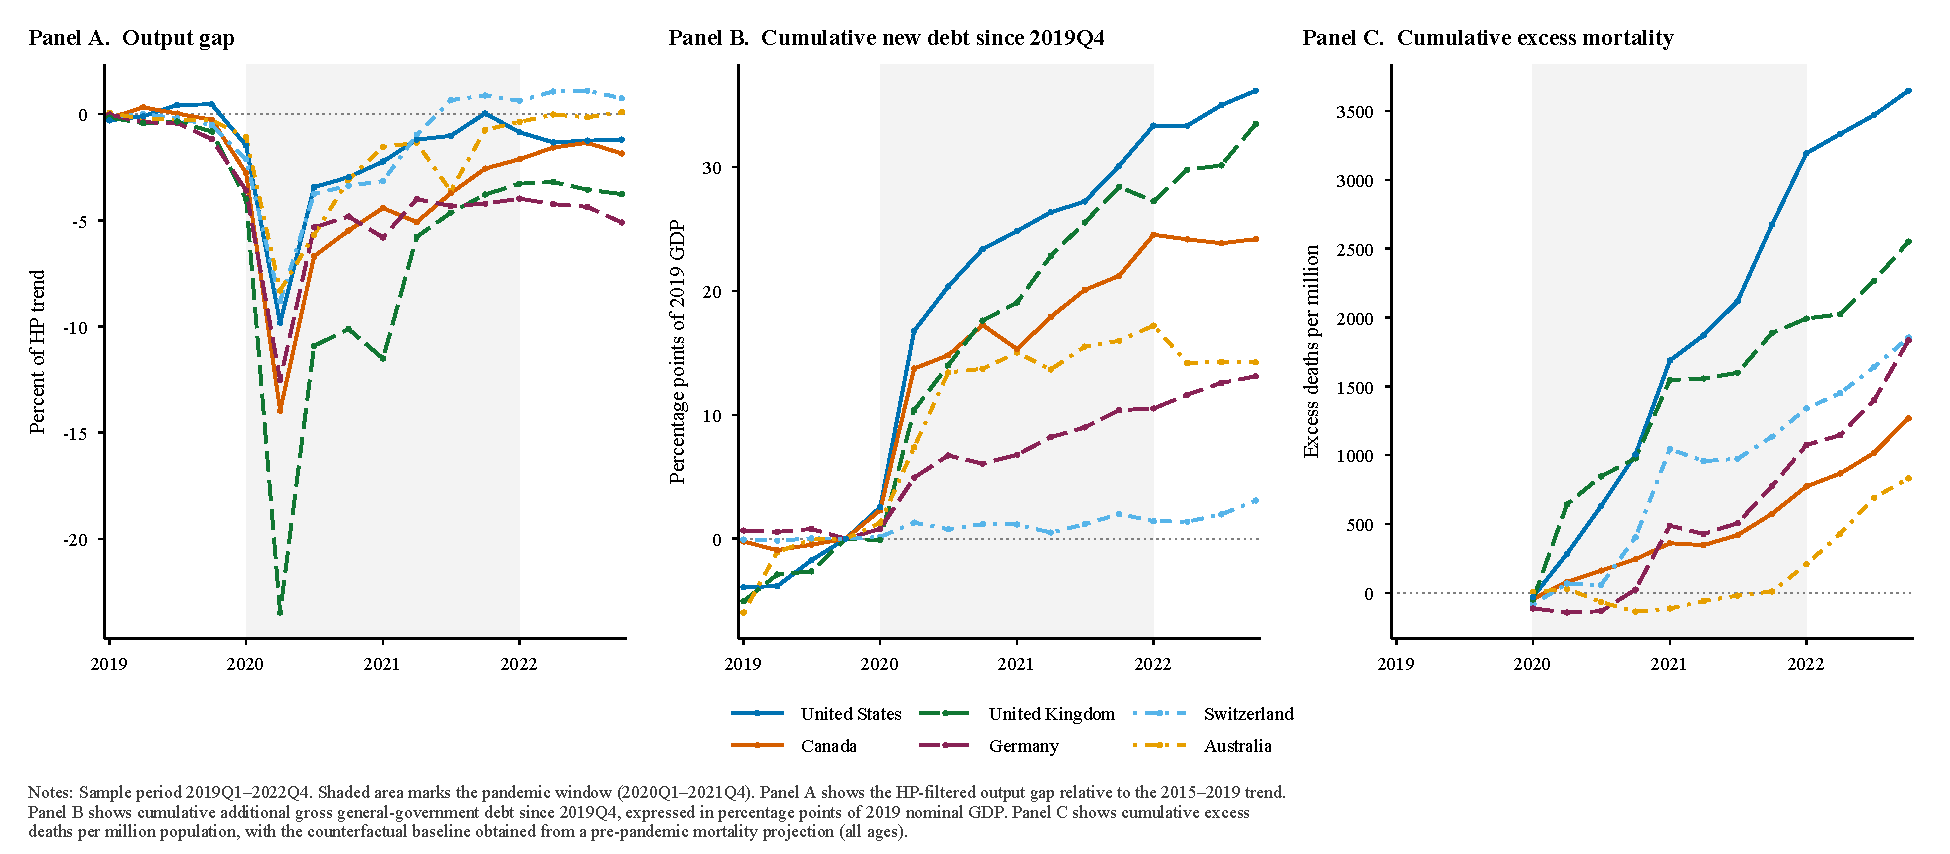
\includegraphics[width=\textwidth]{Files/text/main/outcomes_y_cumdebt_excess_aer.pdf}
    \caption{Pandemic Dynamics: Infection Prevalence, Excess Mortality, 
    and Containment}
    \label{fig:planing_horizon}
\end{figure}


% --- Positioning against existing literature ---

A growing literature has formalized subsets of this problem. \citet{alvarez2020} solve for the optimal lockdown trajectory of a planner trading off fatalities against output costs, while treating the economy as a linear production function with no fiscal dimension. \citet{eichenbaum2021macro} endogenize the behavioral recession by embedding susceptible-infected-removed model (SIR) dynamics into a macroeconomic equilibrium, yet the government's only instrument is a Pigouvian containment tax---no fiscal compensation or debt dynamics enter the problem. \citet{KaplanMollViolante2020} come closest to the full trilemma: they integrate SIR dynamics into a heterogeneous-agent model with both lockdown and fiscal transfers, constructing a pandemic possibility frontier that maps policy combinations to the joint distribution of mortality and economic welfare losses. Their analysis establishes the binding health--economy trade-off and demonstrates that fiscal transfers reshape its distributional incidence. However, government debt enters as a residual accounting identity, not as an optimization target, and fiscal policy is modeled as undifferentiated lump-sum transfers rather than as a composition of instruments with distinct transmission mechanisms.\footnote{For a systematic comparison of modeling approaches in the pandemic-macro literature, see Table~\ref{tab:structured_comp} in Appendix~\ref{app:structured_comp}.}

Three gaps emerge from this body of work. First, no existing framework incorporates fiscal sustainability as a co-equal optimization target alongside health protection and output stabilization---the problem remains a dilemma rather than a trilemma. Second, the fiscal instruments available to the planner have not been disaggregated by their transmission mechanism which generate qualitatively different impact, dynamic profiles and carry different fiscal costs, losing the whole information about the optimal policy mix. Third, the instrument-specific structural parameters that govern the composition problem have not been estimated jointly under pandemic conditions using a transmission-mechanism-based disaggregation---existing cross-country evidence (Deb et al., 2021) benchmarks aggregate fiscal effectiveness but not compositional optimality. 

Closing these three gaps enables an analysis that no existing framework can deliver: given the containment trajectory that the prevailing epidemiological pressure necessitates, the planner can determine the optimal fiscal composition across demand injection and capacity preservation at each point in the pandemic, trace how this composition shifts as the state evolves, and quantify the output and debt consequences of deviating from it. This yields both a retrospective assessment of observed fiscal packages---identifying the excess debt attributable to suboptimal instrument choice---and a prospective benchmark for policymakers confronting future crises that share the pandemic's structural characteristics.

%Containment Intensity raus?


% --- Contributions ---

%Überarbeiten wenn Section fertig
To analyze this question, this paper makes three contributions. First, I develop a formal optimization framework---an iterative Linear-Quadratic Regulator (iLQR) following \citet{bertsekas2017dynamic}---that solves the full trilemma: the planner jointly optimizes containment intensity $S_k$ and the fiscal instruments $F_k^{DI}$ and $F_k^{CP}$ across the multi-dimensional state space $(y_k, d_k, b_k, \theta_k)$, capturing the bilinear interactions between containment and economic persistence that define the pandemic trilemma. Existing approaches solve simpler variants of this problem: Alvarez et al.\ (2021) apply Pontryagin's maximum principle to a single-instrument continuous-time problem, and \citet{eichenbaum2021macro} solve a Ramsey problem over a scalar containment tax. The iLQR extends this to a multi-instrument setting while preserving analytical tractability: the backward Riccati recursion yields time-varying feedback gains $K_k$ that are directly interpretable as the planner's marginal policy response to state deviations, without requiring numerical value function iteration over a high-dimensional state space.%\footnote{The bilinear term $\phi_S S_k \theta_k$ renders the full problem non-convex. The iterative linearization converges to a local optimum. %In the economically relevant region---where the planner responds monotonically to rising infections---local and global solutions coincide, as verified numerically in Appendix~\ref{app:convergence}.} The resulting state-dependent feedback law $u_k^* = -K_k x_k$ yields closed-form optimality conditions (Appendix~\ref{app:optimality}) that characterize the optimal policy trajectory---including the optimal intensity, timing, and composition of the fiscal response---as a function of the evolving state of the system. The quadratic objective penalizing $(y_k, d_k, b_k)$ can be interpreted as a second-order approximation to a welfare function in which the planner assigns explicit weights to output stabilization, mortality reduction, and fiscal sustainability---a Tinbergen-style formulation that takes the multi-objective nature of pandemic policy as given rather than deriving it from a single representative agent's preferences.\footnote{This abstracts from the distributional dimension emphasized by \citet{KaplanMollViolante2020}. The present framework addresses a logically prior question: what is the optimal \textit{aggregate} fiscal composition? The distributional incidence of a given composition is a complementary but distinct problem.}

Second, I construct a new daily micro-level database of 2,290 fiscal policy measures across all 38 OECD member states during 2020--2021 \citep{pesenti2025}. Unlike existing databases that aggregate fiscal responses at the package level, this dataset disaggregates individual measures by instrument type, target group, and IMF fiscal accounting category---the granularity required to operationalize the distinction between demand injection and capacity preservation and thus to adress it in the analyisis. Each of the 49 policy instrument codes is mapped to the theoretical categories (DI or CP) based on a transparent classification protocol that identifies the primary transmission channel. The whole  classification is documented in detail in Section~\ref{sec:classification} or in \citep{Codebook}. 

%instruments that sustain aggregate expenditure through direct income replacement are classified as demand injection, while instruments that preserve productive capacity by maintaining employment relationships, firm solvency, or sectoral viability are classified as capacity preservation.Without this disaggregation, the composition question cannot be empirically addressed: aggregate fiscal impulse measures conflate instruments with fundamentally different transmission mechanisms and fiscal cost profiles.


%EMPIRICAL: DAILY DATA-> GANZER ABSATZ ÜBERARBEITEN
Third, I estimate the structural parameters of the transition system to solve for the optimal trajectory using panel Local Projections \citep{jorda2025} across 38 OECD economies during 2020--2021. 

%The identification strategy exploits cross-country variation in fiscal composition conditional on comparable containment trajectories. A two-stage approach first estimates the policy reaction function---fiscal composition as a function of containment stringency, pre-crisis fiscal position, and institutional characteristics---and then uses deviations from predicted composition as identifying variation.\footnote{The exclusion restriction requires that residual variation in fiscal composition affects economic outcomes only through the fiscal channel. Section~\ref{sec:identification} discusses potential threats, including the possibility that political economy variables driving composition choices (government ideology, coalition structure) independently affect expectations and hence outcomes.} The estimated parameters calibrate the theoretical model and enable two counterfactual exercises. The primary exercise takes each country's observed containment path as given and computes the conditionally optimal fiscal composition---quantifying the excess debt attributable to suboptimal instrument choice, holding the containment trajectory constant. This conditional design reflects the institutional reality that fiscal authorities responded to containment decisions rather than determining them, and isolates the margin over which fiscal policymakers had actual discretion. A secondary exercise computes the fully optimal trajectory across all three instruments, providing an upper bound on the welfare gains from joint optimization of containment and fiscal policy.

% --- Preview of results ---

The main findings are as follows. \textsc{[Placeholder -- to be completed after
estimation.]}

%\textsc{[Result 1: Estimated structural parameters.]} The demand injection multiplier $\hat{\alpha}_F^{DI}$ is estimated at \textsc{[XX]}, while the capacity preservation effectiveness $\hat{\eta}$ is \textsc{[XX]}. The fiscal cost of capacity preservation $\hat{\kappa}_F^{CP}$ is \textsc{[XX]} lower than that of demand injection $\hat{\kappa}_F^{DI}$, reflecting \textsc{[the lower realized cost of guarantees and conditional instruments / the partial recovery of loans and guarantees]}.

%\textsc{[Result 2: Optimal composition trajectory.]} The optimal fiscal mix shifts over the pandemic: during the initial containment phase (high $S_k$, rapidly rising $\theta_k$), the planner allocates \textsc{[XX\%]} of the fiscal envelope to capacity preservation, declining to \textsc{[XX\%]} as containment is relaxed and demand injection becomes the dominant channel. The \textsc{[crossover point / transition]} occurs at approximately \textsc{[quarter XX]}, when the output gap exceeds \textsc{[XX\%]}.

%\textsc{[Result 3: Counterfactual -- conditional optimum.]} Holding each country's observed containment path fixed, the conditionally optimal fiscal composition would have reduced cumulative excess debt by \textsc{[XX]} percentage points of GDP on average across the OECD, with the largest gains in \textsc{[countries with heavy DI tilt during early containment]}. The cross-country variance in excess debt attributable to composition is \textsc{[XX]} percentage points.

%\textsc{[Result 4: Counterfactual -- full optimum.]} Joint optimization over containment and fiscal policy yields additional welfare gains of \textsc{[XX]}, suggesting that the composition margin accounts for approximately \textsc{[XX\%]} of the total welfare distance between observed policy and the unconstrained optimum.

% --- Related literature ---
This paper builds up and contributes to three strands of literature. First, it extends the pandemic-macro modeling literature that integrates SIR dynamics with macroeconomic frameworks \citet{Atkeson2020, eichenbaum2021macro, alvarez2021, KaplanMollViolante2020, Jones2021, acemoglu2021} by incorporating fiscal sustainability as an explicit optimization objective and disaggregating fiscal instruments by transmission mechanism. Second, it contributes to the fiscal multiplier literature \citet{blanchard2002, ramey2018, romer2010} by estimating instrument-specific multipliers under pandemic conditions, where Keynesian supply shocks \citet{guerrieri2022} and voluntary demand reductions \citet{GOOLSBEE2021} render pre-crisis estimates unreliable. Third, it contributes to the empirical literature on cross-country fiscal responses to COVID-19 \citet{deb2021,chetty2020, Autor2022} by providing the first micro-level database with instrument-level granularity and source documentation across all OECD member states, enabling compositional analysis beyond aggregate fiscal impulse comparisons.

% --- Motivation / policy relevance ---

The question addressed here is not only of historical interest. The fiscal legacy of
the pandemic---average OECD government debt increased by approximately \textsc{[XX]}
percentage points of GDP between 2019 and 2021---directly shaped the fiscal space
available when subsequent shocks materialized. The inflation surge of 2022--2023
raised sovereign borrowing costs across advanced economies \citep{jorda2023}; the
energy crisis following the invasion of Ukraine required additional fiscal responses in
an environment of already elevated debt; and the prevailing macroeconomic uncertainty
continues to constrain fiscal policy options. Countries that achieved comparable
health and economic outcomes during the pandemic but at lower fiscal cost---through
more effective instrument composition---entered this sequence of subsequent shocks in
a structurally stronger position. Understanding which fiscal strategies achieved this
outcome, and why, is therefore directly relevant to the current fiscal policy
environment and to the management of future crises that share the pandemic's
structural characteristics.

% --- Roadmap ---

The paper proceeds as follows. Section~\ref{sec:trilemma} establishes the four
constitutive properties of the pandemic trilemma and its structural uniqueness relative
to other crisis types. Section~\ref{sec:model} develops the iLQR optimization
framework. Section~\ref{sec:data} describes the micro-level fiscal policy database.
Section~\ref{sec:estimation} presents the estimation strategy and structural parameter
estimates. Section~\ref{sec:results} reports the optimal composition trajectories and
counterfactual exercises. Section~\ref{sec:conclusion} concludes.


\section{The Pandemic Trilemma}
\label{sec:trilemma}

This section formalizes the trilemma by identifying four constitutive properties of the pandemic environment---exogenous shock with endogenous lethality, contractionary suppression instruments, heterogeneous fiscal compensation channels, and endogenous fiscal feedback---and establishing their circular interdependence. Each property is developed with reference to the empirical literature and introduces the variables and parameters that enter the optimization framework in Section~\ref{sec:planner}. I then apply the four properties as a diagnostic to alternative crisis types, establishing that the pandemic is the only configuration in which all four operate simultaneously within a tractable planning horizon.

%Hall, Jones und Klenow (2020) bringen ein Argument für die höhere Gewichtung von Lives

%% ============================================================
\subsection{Constitutive Properties}
\label{subsec:properties}
%% ============================================================


%% --- Property 1 ---
\subsubsection*{Property 1: Exogenous Shock with Endogenous Dynamics}


A pandemic begins with the introduction of a novel pathogen into the population. I denote the pandemic pressure at time $k$ by $\theta_k$, which I refer to as the viral prevalence. The initial outbreak constitutes an exogenous shock---it originates outside the economic system and is not the result of endogenous market dynamics or policy failure. I represent this shock by a stochastic disturbance $\varepsilon_k$.

The defining characteristic of a pandemic shock is its endogenous growth dynamic: in the absence of intervention, each infected individual transmits the virus to more than one susceptible person, causing the number of infections to grow over time. I capture this by a persistence parameter $\rho_\theta > 1$ (similar to the logic of the reproduction rate during the pandemic), implying that viral prevalence grows exponentially if left unchecked \citep{Atkeson2020, alvarez2021, eichenbaum2021macro}.\footnote{The linear specification abstracts from the susceptible-depletion mechanism of the full SIR framework, where the effective reproduction rate declines endogenously as the susceptible population shrinks. This 
linearization is appropriate for the model horizon (2020--2021), during 
which the pandemic evolved in discrete policy-interrupted waves rather than 
a single depletion arc, and variant emergence repeatedly replenished the 
effective susceptible pool. Residual nonlinearities---including behavioral 
adaptation and immunity waning---are absorbed by the stochastic disturbance 
$\varepsilon_k$.} It is the lethality of the pathogen that transforms this explosive dynamic into a policy imperative: a non-lethal pathogen with $\rho_\theta > 1$ would spread but impose no mortality cost of sufficient magnitude to warrant contractionary public health interventions. When the pathogen is lethal, unchecked exponential growth overwhelms the healthcare system and generates catastrophic mortality \citep{Jones2021, Barro2020}---establishing the necessity of active policy intervention at the cost of economic contraction (Property~2).

This property distinguishes the pandemic shock qualitatively from an impulse shock---such as an earthquake or a one-off financial disruption---where the disturbance dissipates naturally over time ($\rho < 1$) and the system returns to equilibrium without active intervention \citep{jorda2022longer}. These potential consequences are captured by the state variable: \textit{excess mortality} ($d_k$), defined as the deviation of the periodic death rate from its historical seasonal average encompassing both direct COVID-19 deaths and indirect deaths attributable to avoidance of care and healthcare system overload \citep{Msemburi2023WHO, owid_em}. I denote the parameter governing the transmission from infections to deaths by $\delta_\theta$. Crucially, the biological lag between infection and death implies that mortality in period $k+1$ is already determined by the current viral prevalence $\theta_k$ and thus predetermined from the planner's perspective. Consequently, the planner's intervention $S_k$---which suppresses transmission to $\theta_{k+1}$---only impacts mortality starting from period $k+2$. This relationship is given by:

\begin{equation}
    d_{k+2} = \delta_\theta \, \theta_{k+1}, \qquad \text{with} \quad \theta_{k+1} = \rho_\theta \theta_k+\epsilon_k
    \label{eq:mortality_intro}
\end{equation}

The interaction between the lethality parameter $\delta_\theta$ and the transmission potential $\rho_\theta$ plays a decisive role. If $\delta_\theta = 0$---that is, if the virus were non-lethal---or if the pathogen were not transmissible ($\rho_\theta = 0$), there would be no reason for the planner to suppress $\theta_{k+1}$. This logic is formally derived in Appendix \ref{app:Theta import}, which proves that the necessity of a trade-off-inducing policy ($S_k > 0$) depends strictly on the joint condition of positive lethality ($\delta_\theta > 0$) and active transmission ($\rho_\theta > 0$). Absent this conjunction, the suppression strategy becomes orthogonal to health outcomes, and no mortality costs or behavioral responses would arise.


\medskip
\noindent\textit{Summary.} Property~1 introduces the epidemiological state: the infection rate $\theta_k$ (self-reinforcing with $\rho_\theta > 1$), the mortality outcome $d_k$ (driven by $\delta_\theta$), and the exogenous shock $\varepsilon_k$. Together, they establish that the planner must act to suppress viral prevalence, as the system is unstable without intervention.


%% --- Property 2 ---
\subsubsection*{Property 2: Suppression Instrument}
%Maybe NPI's noch unterscheiden nach der Art->bzw mein Index besser!
Given the necessity of intervention established by Property~1, the planner's primary tool to suppress viral transmission during a pandemic is \textit{non-pharmaceutical interventions} (NPIs): measures including, business closures, restrictions on gatherings, school closings, restrictions on internal movement as well as international travel controls and stay-at-home orders. I denote the intensity of these measures at time $k$ by $\Sk$, where $\Sk = 0$ represents the absence of restrictions and $\Sk = 1$ represents a complete lockdown in every aspect. 

NPIs suppress viral prevalence by reducing human contact \citep{Flaxman2020}. I denote the effectiveness of this suppression by the parameter $\phi_S > 0$. Crucially, NPIs do not remove a fixed number of infections from the population; rather, they reduce the rate at which existing infections generate new ones. Each unit of suppression $S_k$ reduces the transmission potential $\rho_\theta$ by the fraction $\phi_S$, yielding an effective reproduction rate $\rho_\theta^{\text{eff}}(S_k) = \rho_\theta(1 - \phi_S S_k)$. Combining this with the mortality transmission from Property~1, the full two-period channel from policy action to health outcome is:
%
\begin{equation}
    d_{k+2} = \delta_\theta \cdot \underbrace{\bigl[\rho_\theta (1 - \phi_S S_k) \, \theta_k + \varepsilon_k\bigr]}_{\theta_{k+1}} 
    \label{eq:excess dynamics}
\end{equation}
%
This equation encodes two features that are central to the planner's problem. First, the suppression effect is multiplicative in the current level of prevalence: at high $\theta_k$, each unit of lockdown prevents more infections---and therefore more deaths---than at low $\theta_k$. The marginal health benefit of suppression, $\partial d_{k+2} / \partial S_k = -\delta_\theta \rho_\theta \phi_S \theta_k$, is state-dependent and vanishes as the pandemic recedes (see Appendix \ref{app:Theta import}). Second, the planner does not control the infection level or the death rate directly but only the growth rate of the epidemic. When $\phi_S S_k$ is sufficient to push $\rho_\theta^{\text{eff}}$ below unity, infections decline; otherwise, they continue to grow despite the intervention. This threshold property---$\rho_\theta^{\text{eff}} < 1$ requires $S_k > \frac{1 - 1/\rho_\theta}{\phi_S}$---implies a minimum lockdown intensity below which suppression is ineffective at reversing the epidemic trajectory.

The central feature of Property~2 is that the channel through which NPIs suppress viral transmission---restricting human interaction---simultaneously reduces the volume of economic activity. Containment measures close businesses, idle labor, and curtail the flow of goods, services, and persons that constitutes aggregate economic output. This duality is not a matter of calibration or implementation; it is inherent to the nature of any instrument that operates through contact reduction.

To formalize this, I introduce the next state variable \textit{output gap} ($y_k$): the percentage deviation of real GDP from its potential trend, where $y_k = 0$ represents normal economic conditions and $y_k < 0$ represents a recession. The contractionary effect of NPIs on output is governed by the parameter $\alpha_S > 0$. Every unit of suppression $\Sk > 0$ therefore simultaneously implies some values of:
%
\begin{alignat}{2}
&\text{Epidemiological benefit:} &\qquad \Delta\theta &= -\phi_S \, \Sk < 0 \label{eq:S_health}\\[4pt]
&\text{Economic cost:} &\qquad \Delta y &= -\alpha_S \, \Sk < 0 \label{eq:S_econ}
\end{alignat}
%

The suppression instrument cannot control the epidemiological shock without simultaneously destabilizing the economic state. This dual impact is structural: it arises from the fact that $\alpha_S$ and $\phi_S$ are both strictly positive and operate through the same policy variable.
 
Beyond the direct contractionary effect of mandated containment, the pandemic generates an additional output cost through the behavioral response. When individuals observe rising death tolls, they voluntarily reduce economic activity independently of any government-mandated restrictions \citep{GOOLSBEE2021} making it a do or die strategy for the social planer as he can control it over the level of infection (or the lethality). I capture this channel through the parameter $\beta_d < 0$, which governs the output response to the mortality flow ($d_k$) and is commonly referred to as the \textit{fear term}. %Literatur das 50-60% der reduktion davon kamen?

A natural objection to Property~2 is that alternative instruments, such as testing, might control the pandemic without suppressing economic activity, thereby dissolving the contractionary link. However, testing capacity constitutes a complement to, rather than a substitute for, NPIs \citep{repec:nbr}. Critically, testing does not alter the biological parameters driving the pandemic: it reduces neither the inherent transmissibility ($\rho_\theta$) nor the lethality ($\delta_\theta$) of the virus. Instead, it operates exclusively through the suppression channel $S_k$. By identifying infected agents, testing enables targeted isolation---which remains a form of NPI. Ideally, this improves the efficiency of the intervention, increasing the ratio of epidemiological benefit ($\phi_S$) to economic cost ($\alpha_S$) by replacing broad lockdowns with specific quarantines. However, testing cannot eliminate the contractionary effect ($\alpha_S > 0$) since even targeted isolation disrupts economic transactions. Moreover, the net effect on the efficiency ratio is ambiguous. Higher detection rates may intensify responses, though the net effect on the efficiency ratio is theoretically ambiguous. 
%Thus, testing modulates the parameter ratio but does not resolve the structurally contractionary nature of suppression.

Vaccination, by contrast, is the instrument that dissolves the trilemma by invalidating Property~2. It operates through both channels: reducing viral transmission among the immunized population (lowering $\rho_\theta$) and reducing the lethality of breakthrough infections (lowering $\delta_\theta$)---which, as demonstrated in Appendix~\ref{app:Theta import}, is the critical mechanism. Crucially, vaccination achieves both effects without operating through the suppression channel $S_k$---it requires no restriction of economic activity \citep{Giordano2021V}, thereby eliminating the contractionary link that constitutes Property~2. However, effective vaccines were not widely available until mid-2021, and the critical vaccination thresholds required to sustainably decouple mortality from infection rates were not reached in most OECD economies until the end of 2021 \citep{OECD2021}. Consequently, for the main phase of the pandemic (Q1 2020--Q4 2021)---the period during which critical policy decisions were taken \citep{Hale2021}---NPIs remained the only available suppression instrument, and were thus inherently contractionary.

\begin{figure}[H]
    \centering
    
\includegraphics[width=\textwidth]{fig_theta_excess_stringency.pdf}
    \caption{Pandemic Dynamics: Infection Prevalence, Excess Mortality, 
    and Containment}
    \label{fig:planing_horizon}
\end{figure}


\noindent Figure~\ref{fig:planing_horizon} illustrates with the OECD average the 
mechanism through which vaccination dissolves the trilemma. During Waves~1--3, infection prevalence and excess mortality move in parallel, and governments maintain elevated containment. With the onset of Wave~4 (Omicron, late 2021), the relationship breaks: infection prevalence reaches its pandemic peak, yet excess mortality declines sharply---reflecting the reduction in $\delta_\theta$ achieved by widespread vaccination. Governments respond by withdrawing containment to near-zero levels despite record case counts. This decoupling is precisely the condition 
$\delta_\theta \to 0$ formalized above: once the fatality rate 
falls sufficiently, the rational to act vanishes, and the trilemma ceases to bind. This observation defines the planner's  horizon: the trilemma is operative from Q1\,2020 through Q4\,2021---the period during which the joint condition of positive lethality ($\delta_\theta > 0$) and absence of effective vaccination necessitated the health--economy--fiscal trade-off. Beyond the terminal date, the planner faces no further trilemma and deals exclusively with the fiscal legacy of the crisis.
%Anpassen

\medskip
\noindent\textit{Summary.} Property~2 introduces the suppression instrument $S_k$, its epidemiological effectiveness $\phi_S$, its direct economic cost $\alpha_S$, the behavioral cost $\beta_d$ driven by observed mortality, and the output gap $y_k$. It establishes that pandemic suppression is inherently contractionary: the planner cannot protect health without damaging the economy unless an effective vaccine is available.
%================================================================
% Property 3: Fiscal Compensation Instruments
% Revised: April 2026
% ================================================================

\subsubsection*{Property 3: Fiscal Compensation Instruments}

Given that pandemic suppression is inherently contractionary (Property~2), the social planner requires compensating instruments to stabilize the economic state. The pandemic damages the economy through two main channels. Containment and behavioral retrenchment directly reduce the level of output by restricting economic activity and suppressing expenditure. Simultaneously, the prolonged disruption erodes the economy's capacity to recover---through firm failures, dissolution of employment relationships, and disruption of supply chains---prolonging the contraction beyond the duration of the shock itself. To address these two channels, the social planner has to target these channels separately (level and persistence).

The first category, demand injection ($F^{DI}_k$) comprises measures that directly increase the flow of disposable income in the economy: stimulus checks (such as the U.S.\ Economic Impact Payments under the CARES Act), direct transfers to households (such as the Australian JobSeeker supplement or the Japanese universal cash transfer of \textyen100,000 per resident), and tax reductions that raise disposable income (such as the German temporary VAT reduction from 19\% to 16\% in H2~2020). These instruments transmit through the standard Keynesian multiplier channel and are widely used in depressed economic environment, shifting the output gap by $\alpha_{DI} > 0$ per unit deployed. \footnote{Pre-pandemic estimates place expenditure multipliers in a range of approximately 0.5 to 1.5 \citep{ramey2018, blanchard2002}.}

However, applying these instrument to a pandemic environment is questionable on both theoretical and practical grounds. The pandemic  recession is not a demand shock but a supply disruption induced by containment \citep{guerrieri2022}: businesses are closed by government order, not by insufficient demand. Injecting purchasing power into an economy where the supply of goods and services is physically restricted cannot translate into expenditure at the usual rate \citep{chetty2020, coibion2020}. This raises the question whether $\alpha_{DI}$ under pandemic conditions retains a meaningful magnitude, is merely delayed, or vanishes entirely.


The second category, capacity preservation ($F^{CP}_k$), encompasses measures that maintain the existing productive structure of the economy: short-time work schemes (such as the Swiss \textit{Kurzarbeitsentsch\"{a}digung} or the UK Coronavirus Job Retention Scheme), payroll subsidies, and government-guaranteed loans (such as the French \textit{Pr\^{e}ts Garantis par l'\'{E}tat} or the German KfW-Sonderprogramm). Unlike demand injection, capacity preservation targets the persistence of the shock rather than his level. When a lockdown closes a firm, CP does not restore its output---the firm remains closed regardless. What CP prevents is the destruction of firm-worker matches, supplier relationships, and organizational capital that would otherwise dissolve during the shutdown---precisely the amplification mechanism that \citet{guerrieri2022} identify as propagating the initial sectoral shock. The preservation effect materializes only once containment eases and preserved capacity resumes production, making CP a structurally delayed instrument whose effectiveness depends on the depth of the contraction it is deployed against.

Combining the pandemic shocks from Property~2 with the fiscal instruments above, the output evolves according to:

\begin{equation}\label{eq:output}
    y_{k+1} \;=\; \underbrace{\bigl(\rho_y + \psi\, S_k - \eta_p\, F^{CP}_{k-1}\bigr)}_{\equiv\;\rho^{\text{eff}}_k}\; y_k
    \;-\; \alpha_S\, S_k
    \;+\; \alpha_{\textit{DI}}\, F^{DI}_{k-1}
    \;-\; \beta_d\, d_k.
\end{equation}

\noindent Three features of equation~\eqref{eq:output} merit emphasis. 
First, the effective persistence $\rho^{\text{eff}}_k = \rho_y + \psi\, S_k - \eta_p\, F^{CP}_{k-1}$ is governed by two opposing forces. Containment raises persistence ($\psi > 0$) and capacity preservation lowers it ($\eta_p > 0$). Therefore, the net effect determines the speed of recovery---not the depth of the initial contraction, which is pinned down by the additive terms $\alpha_S$ and $\beta_d$.

Second, CP is effective only when the economy is in recession. The marginal output effect of capacity preservation is $\eta_p\,|y_k|$: at $y_k = 0$, CP has no effect---there is no productive structure at risk. The deeper the contraction, the more matches and relationships face dissolution, and the larger the preservation benefit. This proportionality provides a formal rationale for the front-loading of CP programs observed across OECD economies during 2020, and implies that the optimal fiscal composition is state-dependent rather than fixed. The empirical counterpart is that corporate insolvencies across OECD economies fell by 17\% on average in 2020 relative to 2019 despite the deepest recession since the Great Depression \citep{djankov2021, banerjee2021}---a pattern difficult to reconcile without the structural preservation channel formalized here.

Third, DI operates through a conventional level channel: $\alpha_{\textit{DI}}\, F^{DI}_{k-1}$ shifts the output gap by a constant amount per unit deployed, independently of the economic state. This transmission mechanism is well-established for standard recessions where consumption channels are open \citep{ramey2018, blanchard2002}. During a pandemic lockdown, however, containment restrictions constrain the expenditure margin, potentially attenuating the multiplier. \citet{chetty2020} document that U.S.\ stimulus payments during strict containment were largely saved rather than spent, consistent with a blocked demand channel. The present framework nests this possibility: if $\alpha_{\textit{DI}} = 0$, CP is the sole instrument through which fiscal resources translate into output recovery.

The preceding analysis might suggest a straightforward resolution: deploy CP until the persistence reduction offsets the lockdown amplification ($\eta_p\, F^{CP}_{k-1} \approx \psi\, S_k$), then inject demand into an economy whose productive structures are intact. However, this reasoning abstracts from the budgetary consequences of the fiscal package itself. Each instrument that stabilizes the output gap simultaneously augments the government's balance sheet---and the magnitude of this fiscal cost is heterogeneous across categories and in several dimensions not yet established in the literature. To formalize this constraint, I introduce the third state variable: \textit{public debt} ($b_k$), defined as the deviation of the debt-to-GDP ratio from its pre-pandemic level.\footnote{I normalize by pre-pandemic GDP (2019) rather than current GDP and express it in real values. When debt is expressed relative to current output, a recession mechanically inflates the ratio through the denominator even absent any new borrowing. Normalizing by the pre-pandemic level isolates changes in the numerator---the actual stock of government liabilities---which is the object relevant to the planner's decision.}

%
\begin{equation}
    b_{k+1} = (1+r)\, b_k - \gamma_y\, y_k + \kappa^{CP}\, F^{CP}_k + \kappa^{DI}\, F^{DI}_k + c_H\, \theta_k
    \label{eq:debt}
\end{equation}
%
where $r$ is the real interest rate, $\gamma_y > 0$ is the budget semi-elasticity (the automatic stabilizer channel formalized in Property~4), $\kappa^{CP}$ and $\kappa^{DI}$ are the budgetary cost parameters, and $c_H\, \theta_k$ captures pandemic-specific health expenditures.\footnote{See the discussion of health expenditures in the behavioral pandemic cost paragraph above.}

The budgetary cost parameter $\kappa^{CP}$ is not a single number but a weighted average over two structurally distinct sub-categories. Direct capacity preservation---short-time work schemes, payroll subsidies, and direct grants---generates immediate budgetary outlays classified as above-the-line expenditure \citep{imf2022fiscalmonitor}. Loans and guarantees, classified as below-the-line, involve either a net fiscal cost well below unity (loans, where the government creates a financial asset offsetting the cash outflow) or near zero at deployment (guarantees, which generate no immediate outflow but create contingent liabilities whose realized cost depends on the default rate among supported borrowers). The effective raw effect of $\kappa^{CP}$ therefore depends on the composition of the CP package and the realized default rate on contingent instruments.

The joint structure of equations~\eqref{eq:output} and~\eqref{eq:debt} reveals that every unit of output stabilization carries a fiscal price---but this price differs across instruments and varies with the state of the economy. For capacity preservation, the marginal output gain from one additional unit of $F^{CP}$ is $\eta_p\,|y_k|$---proportional to the depth of the recession. The fiscal cost per unit of output gap closed is therefore:
%
\begin{equation}
    \pi^{CP}_k \;\equiv\; 
    \frac{\kappa^{CP}_i}{\eta_p\,|y_k|}
    \label{eq:price_CP}
\end{equation}
%
This price is state-dependent: it falls with the depth of the recession as the preservation benefit grows, and rises toward infinity as the economy approaches full capacity ($y_k \to 0$). CP is cheap when it is most needed and prohibitively expensive when it is not---a property that provides a natural exit criterion for capacity preservation programs. For demand injection, the analogous price is:
%
\begin{equation}
    \pi^{DI} \;\equiv\; 
    \frac{\kappa^{DI}}{\alpha_{\textit{DI}}}
    \label{eq:price_DI}
\end{equation}
%
This price is state-independent---it does not vary with $S_k$, $y_k$, or any other variable in the system. CP dominates DI whenever the recession is sufficiently deep that $\pi^{CP}_k < \pi^{DI}$, which yields the threshold condition:
%
\begin{equation}
    |y_k| \;>\; \frac{\alpha_{\textit{DI}}\;\kappa^{CP}_i}{\eta_p\;\kappa^{DI}}
    \;\equiv\; y^*
    \label{eq:threshold}
\end{equation}
%

Below this threshold, the constant-return DI channel is more cost-effective per unit of debt. Above it, CP delivers more output recovery per fiscal dollar because the preservation benefit scales with the severity of the crisis. The model therefore predicts that the optimal fiscal composition---in terms of both effectiveness and cost---is not fixed but evolves endogenously with the state of the economy, shifting from CP-dominant during the acute contraction to DI-dominant during the recovery. This composition at each stage of the pandemic depends on the current state, on the anticipated trajectory of containment and infections, and on the cumulative fiscal legacy of past decisions---translating the problem into a genuinely dynamic one.


\vspace{5mm}
\noindent\textit{Summary.} Property~3 introduces the fiscal compensation instruments---demand injection ($F^{DI}_k$) and capacity preservation ($F^{CP}_k$), disaggregated based on their transmission channels---and the public debt state ($b_k$). The two instruments operate through fundamentally different channels: DI shifts the output level through a state-independent multiplier $\alpha_{DI}$, while CP reduces the effective persistence of the shock through $\eta_p\, |y_k|$---a benefit proportional to the depth of the recession. Each instrument that stabilizes output simultaneously augments the government's balance sheet, but the fiscal price per unit of stabilization differs across instruments and varies with the pandemic state. These state-dependent prices render the optimal composition and timing of the fiscal response an inherently dynamic problem.


\subsubsection*{Property 4: Endogenous Fiscal Feedback via Automatic Stabilizers}

When NPIs contract economic output (Property~2), the resulting negative output gap triggers two simultaneous and automatic fiscal effects. On the revenue side, the tax base shrinks, reducing government receipts below their pre-pandemic trajectory. On the expenditure side, mandatory transfer programs such as unemployment insurance, social assistance, and housing benefits expand as more individuals satisfy eligibility criteria. The parameter $\gamma_y > 0$ in the debt transition~\eqref{eq:debt} captures the aggregate sensitivity of the budget to the output gap, encompassing both channels in a single semi-elasticity.\footnote{For OECD economies, estimates of the budget semi-elasticity range from approximately 0.35 to 0.65, with a cross-country average around 0.5 \citep{repec:oecd}. The parameter is structurally determined by the tax-to-GDP ratio and the coverage of automatic transfer programs.}

This term operates symmetrically. A negative output gap ($y_k < 0$) widens the deficit through lower revenues and higher mandatory expenditures; a narrowing gap ($y_k \to 0$) reverses both effects, reducing the pace of debt accumulation. The symmetry carries a direct implication for instrument choice: a fiscal instrument whose output effect is large relative to its fiscal cost generates a double dividend---it stabilizes output directly and attenuates the automatic fiscal deterioration indirectly, as the improved $y_k$ feeds back through $\gamma_y$ to slow debt accumulation.

The central contribution of this property is to close the trilemma by establishing that fiscal abstinence is not a feasible strategy \citep{Fornaro2020}. Setting all discretionary instruments to zero ($F_k^{DI} = F_k^{CP} = 0$) in~\eqref{eq:debt} yields:
%
\begin{equation}
    b_{k+1} = (1+r) \, b_k - \gamma_y \, y_k
    \label{eq:debt_no_fiscal}
\end{equation}
%
Since $y_k < 0$ during containment, $-\gamma_y y_k > 0$: debt accumulates even without any discretionary fiscal expenditure. A lockdown without accompanying fiscal measures still erodes the fiscal position---the trilemma cannot be circumvented by fiscal abstinence. Combined with the necessity of suppression established in Property~1, this means that the planner's decision is not whether to deploy fiscal support but which composition to deploy and when---returning the problem to the instrument choice formalized in Property~3.

\vspace{5mm}
\noindent\textit{Summary.} Property 4 introduces the budget semi-elasticity $\gamma_y$ and establishes that fiscal abstinence is an illusion: suppression passively erodes the fiscal position even absent discretionary intervention. The planner's decision is therefore not whether to intervene fiscally, but how to compose the intervention to minimize the joint debt footprint. 

% ============================================================
\subsection{Summary}
\label{sec:Sumary}
% ============================================================
The four properties jointly characterize the structural environment of the pandemic trilemma. First, the system contains multiple simultaneously unstable dimensions: the epidemiological state is explosive without containment ($\rho_\theta > 1$); the output state becomes conditionally unstable under containment without capacity preservation ($\rho^{\text{eff}}_y \to 1$); and the debt state is unconditionally explosive, compounding any fiscal cost incurred during the crisis beyond the planning horizon ($(1+r) > 1$). These instabilities jointly establish the necessity of planner intervention.

Second, every available instrument is structurally coupled across state dimensions. Containment suppresses infections but contracts output directly and through the behavioral response to mortality. Demand injection shifts the output level but augments debt. Capacity preservation reduces the persistence of the shock---a benefit proportional to the depth of the recession---but carries uncertain fiscal costs that depend on the composition of the package and the realized default rate on contingent instruments. No instrument operates on a single dimension, and mortality is not directly controllable, requiring a two-period transmission through the suppression channel.

Third, the marginal costs and benefits of each instrument are state-dependent. The epidemiological benefit of containment vanishes as infections recede. The output effect of capacity preservation scales with $|y_k|$, implying that CP is effective only when the economy is in recession and economically prohibitive once the output gap closes. The fiscal price of CP falls with the depth of the recession, while the price of DI is constant. The optimal instrument composition therefore evolves endogenously with the state of the economy.

Fourth, the system is inescapably constrained: every response to one dimension of the crisis worsens at least one other dimension, and fiscal abstinence worsens the fiscal dimension regardless through the automatic stabilizer channel ($\gamma_y$). The trilemma cannot be circumvented by inaction.

\subsubsection{Structural Uniqueness}

To establish that the pandemic trilemma represents a structurally distinct problem, I apply the four constitutive properties as a diagnostic framework to four alternative crisis types: armed conflict, natural disasters, financial crises, and climate change.\footnote{See Appendix~\ref{subsec:comparison} for the complete diagnostic.} No other crisis type satisfies all four properties simultaneously. Armed conflict and natural disasters fail Property~2: the instruments that address the threat---military mobilization, reconstruction spending---are expansionary rather than contractionary. Financial crises fail Property~1: the shock is endogenous, and the primary interventions work with rather than against economic stabilization. Climate change approximates all four properties in principle, but differs in time scale (decades versus quarters), observability of the health outcome (diffuse versus immediate), and terminal condition: while technological decarbonization can in principle dissolve the climate trilemma---analogous to vaccination dissolving the pandemic trilemma---this resolution operates on a multi-decadal horizon with no guaranteed terminal date. The pandemic is therefore the only crisis type in which all four properties and their interdependence are simultaneously operative within a tractable planning horizon providing a unique situation.



\section{The Planner's Problem}
\label{sec:planner}

The four properties established in Section~\ref{subsec:properties} together define the structural environment of the pandemic trilemma: the instability of the three state dimensions, the cross-dimensional coupling of every available instrument, the state-dependence of marginal costs and benefits, and the infeasibility of fiscal abstinence. This section assembles these elements into the formal decision problem faced by a social planner.

The state vector is $\mathbf{x}_k = (\theta_k,\, d_k,\, y_k,\, b_k)'$, collecting the epidemiological prevalence, observed mortality, output gap, and public debt defined in Section~\ref{sec:trilemma}. The control vector is $\mathbf{u}_k = (S_k,\, F^{CP}_k,\, F^{DI}_k)'$, combining the containment instrument with the two fiscal instruments. The state evolves according to the following transition system:
%
\begin{align}
    \theta_{k+1} &= \rho_\theta\,(1 - \phi_S S_k)\, \theta_k + \varepsilon_k \label{eq:plan_theta}\\[3pt]
    d_{k+1} &= \delta_\theta\, \theta_k \label{eq:plan_d}\\[3pt]
    y_{k+1} &= \bigl(\rho_y + \psi\, S_k - \eta_p\, F^{CP}_{k-1}\bigr)\, y_k - \alpha_S\, S_k + \alpha_{DI}\, F^{DI}_{k-1} - \beta_d\, d_k \label{eq:plan_y}\\[3pt]
    b_{k+1} &= (1+r)\, b_k - \gamma_y\, y_k + \kappa^{CP}\, F^{CP}_k + \kappa^{DI}\, F^{DI}_k + c_H\, \theta_k \label{eq:plan_b}
\end{align}
%
The planner chooses the control sequence $\{\mathbf{u}_k\}_{k=0}^{N-1}$ to minimize a weighted quadratic loss over the planning horizon: \footnote{The quadratic objective~\eqref{eq:objective1} adopts a Tinbergen-style formulation that takes the multi-objective nature of pandemic policy as given, rather than deriving it from a representative agent's preferences---interpretable as a second-order approximation to such a welfare function \citep{woodford2003}.}
%
\begin{equation}
    \min_{\{\mathbf{u}_k\}_{k=0}^{N-1}} \; \mathbb{E}\left\{\tfrac{1}{2}\,\bm{x}_N'\,\bm{Q}_N\,\bm{x}_N
    \;+\; \sum_{k=0}^{N-1}\tfrac{1}{2}\left(\bm{x}_k'\,\bm{Q}_k\,\bm{x}_k
    \;+\; \bm{u}_k'\,\bm{R}_k\,\bm{u}_k\right)\right\}
    \label{eq:objective1}
\end{equation}


%
%with weight matrices:
%
%\begin{equation}
%\begin{aligned}
    %\bm{Q}_k &= \beta^k\,\operatorname{diag}(w_y,\, w_d,\, w_b,\, 0,\, 0), \\
   %\bm{Q}_N &= \beta^N\,\operatorname{diag}(0,\, 0,\, W_b,\, 0,\, 0), \\
    %\bm{R}_k &= \beta^k\,\operatorname{diag}(r_S,\, r_F^{DI},\, r_F^{CP}).
%\end{aligned}
%\label{eq:weights}
%\end{equation}

subject to~\eqref{eq:plan_theta}--\eqref{eq:plan_b} and the non-negativity constraints $S_k, F^{CP}_k, F^{DI}_k \geq 0$. The weighting matrices take the diagonal form $\bm{Q}_k = \beta^k \cdot \text{diag}(0, w_d, w_y, w_b)$ and $\bm{R}_k = \beta^k \cdot \text{diag}(r_S, r_{CP}, r_{DI})$, with terminal matrix $\bm{Q}_N = \beta^{N+1} \cdot \text{diag}(0, 0, 0, W_b)$. The state weights $w_d, w_y, w_b > 0$ reflect the planner's preferences over mortality, output stabilization, and fiscal restraint; the control penalties $r_S, r_{CP}, r_{DI} > 0$ regularize the deployment of each instrument; and $\beta \in (0,1)$ is the discount factor. The terminal weight $W_b$ penalizes debt exclusively: output gaps close endogenously as containment is lifted, and mortality costs are irreversible and already penalized along the trajectory through $w_d$, but debt compounds at rate $(1+r)$ beyond the planning horizon and constrains the fiscal response to subsequent shocks.\footnote{This abstracts from the distributional dimension emphasized by \citet{KaplanMollViolante2020}. The present framework addresses a logically prior question: what is the optimal \textit{aggregate} fiscal composition? The distributional incidence of a given composition is a complementary but distinct problem.}

The transition equations are specified as reduced-form relationships governing the evolution of the state vector, rather than equilibrium conditions derived from household and firm optimization. This places the model in the tradition of optimal policy analysis with reduced-form constraints---an approach with established precedents in the pandemic-macro literature \citep{alvarez2020, acemoglu2021}. The alternative---a fully microfounded DSGE framework---would derive the output dynamics from household and firm optimization, as in \citet{eichenbaum2021macro} and \citet{KaplanMollViolante2020}. However, the output response to containment in such models depends sensitively on functional form assumptions, household heterogeneity, and market structure, none of which bear directly on the fiscal composition question that this paper addresses. Section~\ref{sec:lit} discusses the relationship to this macro-modeling literature in more detail.

This choice of specification enables a decomposition that has not been formulated in the macroeconomic literature on pandemic policy: the separation of capacity preservation from demand injection on the basis of their transmission mechanism---level versus persistence---rather than their budgetary accounting. \citet{guerrieri2022} identify firm exit and job destruction as propagation mechanisms that amplify the initial sectoral shock, providing the theoretical foundation for the persistence channel, but do not formalize capacity preservation as a distinct fiscal instrument operating through this channel. \citet{deb2021} document empirically that emergency lifeline measures are more effective under strict containment while demand-support measures dominate during reopening, but their classification follows budgetary accounting conventions---above-the-line versus below-the-line---rather than the economic transmission channel.\footnote{These categories cut across the distinction drawn here: above-the-line spending includes both demand-oriented measures (transfers, tax cuts) and capacity-preserving measures (short-time work, direct grants), while below-the-line spending captures part but not all of the capacity preservation category (loans and guarantees, but not payroll subsidies).} \citet{gourinchas2021} quantify the firm-failure channel at the micro level, showing that fiscal support reduced SME failure rates by approximately 4.7 percentage points through liquidity preservation rather than demand stimulation---evidence for the persistence mechanism at the firm level that the present framework formalizes at the macro level. Together, the existing literature and the formalized framework motivate the central research question of this paper: \textit{What is the optimal composition of fiscal support between capacity preservation and demand injection over the course of a pandemic, and what are the costs—in foregone output stabilization and excess debt—of deviating from this optimum?}

To answer this research question, the remainder of the paper proceeds the following steps. In Section~\ref{sec:estimation} I estimate the structural parameters governing the transmission channels---$\rho_y$, $\psi$, $\eta_p$, $\alpha_S$, $\alpha_{DI}$, and $\beta_d$---from the cross-country panel, identifying the empirical strength and timing of each channel and providing estimates of the effectiveness and fiscal cost of each instrument. Section~\ref{sec:calibration} calibrates the model using these estimates together with country-specific fixed effects and the epidemiological parameters ($\rho_\theta$, $\delta_\theta$, $\phi_S$) obtained from the data. Section~\ref{sec:counterfactuals} uses the calibrated model to solve the planner's minimization problem, constructing an optimal trajectory at the aggregate level and running scenario and country-specific counterfactuals: holding each country's observed pandemic conditions fixed---its containment trajectory, its epidemiological state, and the behavioral response to mortality---to answer which fiscal composition would have minimized the planner's loss given his pandemic conditions they faced and how far each country's realized policy departed from that conditional optimum.

Although the empirical analysis identifies how containment ($S_k$) and observed mortality ($d_k$) affect output, the paper does not model the epidemiological dynamics that generate these variables. I therefore fix each country's observed containment trajectory $\{S_k^{\text{obs}}\}$ and the induced epidemiological states $\{\theta_k^{\text{obs}}, d_k^{\text{obs}}\}$ throughout the optimization, and solve only for the fiscal controls. Two considerations motivate this restriction.

First, the epidemiological transition~\eqref{eq:plan_theta} depends on biological parameters ($\rho_\theta$, $\delta_\theta$, $\phi_S$) that lie outside the domain of fiscal policy analysis and that the present framework does not claim to model rigorously. Conditioning on observed containment and the resulting epidemiological trajectory keeps the analysis within the scope of this paper.\footnote{Although the epidemiological dynamics are not targeted in the calibration, I use the fit of simulated $\theta_k$ and $d_k$ against their observed counterparts as a non-targeted moment, providing independent evidence on model validity. See Section~\ref{sec:calibration} for details.}

Second, this restriction reflects the institutional reality of pandemic policymaking rather than a modeling compromise. Governments during the pandemic did not choose containment and fiscal composition jointly: public health authorities set $S_k$ based on epidemiological considerations, treating the protection of life as the binding priority, and finance ministries subsequently chose fiscal instruments to compensate for the economic consequences. The social planner in the present framework therefore faces the same sequential decision structure as real-world governments---taking containment as given and optimizing over the fiscal margin. The resulting problem is both policy-relevant and considerably less studied than optimal containment policy.



% =============================================================
% Section 4 — Empirical Strategy
% =============================================================

\section{Empirics}
\label{sec:estimation}

\subsection{Data and Measurement}
\label{subsec:data}

The analysis draws on a quarterly panel dataset covering all 38 OECD member states. The underlying data span Q1.2015 through Q4.2024, though the estimation sample is substantially narrower. Table~\ref{tab:data_sources} summarizes all variables and sources.

% --- TABLE 1: Variables and Sources ---
\begin{table}[H]
\centering
\caption{Variables and Data Sources}
\label{tab:data_sources}
\scriptsize
\begin{tabular}{@{}lp{7cm}l@{}}
\toprule
\textbf{Variable} & \textbf{Description} & \textbf{Source} \\
\midrule
\multicolumn{3}{@{}l}{\textit{Dependent variables}} \\[3pt]
$y_{ik}$
  & Output gap: \% deviation of real GDP from HP-filtered
    trend (2015--2019, $\lambda = 1600$)
  & \citet{OECDQNA} \\[6pt]
$b_{ik}$
  & Quarterly change in real public debt, normalized
    by 2019 GDP (pp)
  & \citet{OECDQNA} \\[6pt]
\midrule
\multicolumn{3}{@{}l}{\textit{Policy variables}} \\[3pt]
$S_{ik}$
  & Stringency Index, population-weighted (0--100)
  & Own calc.\ (APX); \citet{Hale2021} \\[6pt]
$F_{ik}^{CP}$
  & Capacity preservation (\% of 2019 GDP)
  & Own database (APX) \\[6pt]
$F_{ik}^{DI}$
  & Demand injection (\% of 2019 GDP)
  & Own database (APX) \\[6pt]
$F_{ik}^{H}$
  & Health spending (\% of 2019 GDP)
  & Own database (APX) \\[6pt]
\midrule
\multicolumn{3}{@{}l}{\textit{Epidemiological variables}} \\[3pt]
$d_{ik}$
  & Excess mortality (P-score)
  & \citet{Msemburi2023WHO}; \citet{owid_em} \\[6pt]
$\theta_{ik}$
  & Infection prevalence, estimated from excess
    mortality via country-specific IFRs
  & Own calc.\ (APX); \citet{Levin2020} \\[6pt]
$\text{Vax}_{ik}$
  & Cumulative vaccination doses per capita
  & \citet{Mathieu2021} \\[6pt]
\bottomrule
\end{tabular}

\smallskip
{\scriptsize \textit{Notes:} All fiscal variables normalized by 2019 GDP.
2,301 individual measures classified by transmission channel and aggregated to
country-quarter level. See Data Appendix for the classification protocol.}
\end{table}

% --- PROSE: follows table order top to bottom ---

\noindent The output gap $y_{ik}$ is measured as the percentage deviation of
quarterly real GDP from its Hodrick--Prescott-filtered trend, estimated
exclusively on pre-pandemic data (2015--2019, $\lambda = 1600$) and projected
forward, yielding a country-specific counterfactual that is comparable across
countries in percentage-point terms.%
\footnote{Applying the HP filter to the full sample including 2020--2021 would
pull the estimated trend downward, mechanically reducing the measured output gap.
The pre-pandemic-only estimation ensures that counterfactual potential output
reflects the economy's trajectory absent the pandemic shock.}
The debt variable $b_{ik}$ is the quarterly first difference of real public debt,
normalized by 2019 GDP rather than contemporaneous GDP to isolate actual debt
accumulation from denominator effects: a recession mechanically inflates the
conventional debt-to-GDP ratio even without new borrowing. The fixed denominator
ensures that $b_{ik}$ is comparable across countries and over time in
percentage-point terms.%
\footnote{The real debt series deflates nominal general government gross debt by
the GDP deflator. Robustness checks using nominal debt and controlling for the
inflation rate yield qualitatively identical results
(Section~\ref{subsec:robustness}).}

The fiscal variables $F_{ik}^{CP}$, $F_{ik}^{DI}$, and $F_{ik}^{H}$ are
constructed from a novel micro-level database of 2,301 individual policy measures
across all 38 OECD member states, building on and substantially extending an
initial draft by \citet{lacey2021}. The database records each measure at daily
frequency with its announcement date, description, primary source, and fiscal
cost (in local currency and as \% of 2019 GDP). The classification distinguishes instruments by their primary economic transmission mechanism rather than by recipient or administrative category---the operationalization required by the theoretical framework in Section~\ref{sec:trilemma}. Table~\ref{tab:fiscal_classification} details the composition of each channel. The full classification protocol and a
high-frequency descriptive analysis for all 38 OECD countries are documented in
the Data Appendix (Appendix~\ref{app:data}).

% --- TABLE 2: Fiscal Classification (embedded in fiscal discussion) ---
\begin{table}[H]
\centering
\caption{Fiscal Instrument Classification}
\label{tab:fiscal_classification}
\scriptsize
\begin{tabular}{@{}llr@{}}
\toprule
\textbf{Channel} & \textbf{Instruments} & \textbf{Measures} \\
\midrule
\multicolumn{3}{@{}l}{\textit{Capacity Preservation ($F^{CP}$)}} \\[3pt]
\quad Above-the-line
  & Short-time work, payroll subsidies, direct grants
  & 948 \\[3pt]
\quad Below-the-line
  & Government loans, credit guarantees
  & 400 \\[6pt]
\multicolumn{3}{@{}l}{\textit{Demand Injection ($F^{DI}$)}} \\[3pt]
\quad Transfers
  & Cash transfers, unemployment top-ups, ad-hoc benefits
  & 346 \\[3pt]
\quad Tax measures
  & Income tax relief, VAT reductions, tax credits
  & 162 \\[3pt]
\quad Demand stimulus
  & Infrastructure, green investment, tourism support
  & 38 \\[6pt]
\multicolumn{3}{@{}l}{\textit{Health ($F^{H}$)}} \\[3pt]
\quad
  & Medical procurement, hospital capacity, vaccine rollout
  & 232 \\[6pt]
\midrule
\multicolumn{2}{@{}l}{\textit{Excluded: Tax deferrals (IMF Cat.\ 3)}}
  & 154 \\[3pt]
\multicolumn{2}{@{}l}{\textit{Excluded: Unclassified and excluded policy codes}}
  & 21 \\[3pt]
\midrule
\multicolumn{2}{@{}l}{\textbf{Total}}
  & \textbf{2,301} \\
\bottomrule
\end{tabular}

\smallskip
{\scriptsize \textit{Notes:} Classification by primary transmission mechanism,
not by recipient or administrative category. Below-the-line CP adjusted to 35\%
estimated take-up rate in the debt equation (25\%/50\% robustness). Tax deferrals
excluded as realized fiscal cost approaches zero. Full protocol in Data Appendix
(Appendix~\ref{app:data}).}
\end{table}

\noindent Excess mortality $d_{ik}$---the deviation of all-cause deaths from a
projected seasonal baseline---is the preferred measure of pandemic health impact.
Unlike reported COVID-19 deaths, which depend on testing capacity, health
infrastructure and cause-of-death attribution practices that varied widely across
countries, excess mortality captures both direct viral fatalities and indirect
deaths from healthcare system overload, deferred care, and resource diversion
\citep{Msemburi2023WHO}. It is recorded with coverage across all OECD countries regardless of testing infrastructure, making it comparable across countries and over time. Excess mortality also enters the output equation as the fear term $d_{ik}$, controlling for voluntary reductions in economic activity: \citet{GOOLSBEE2021} show that observed lethality---not case counts---was the primary driver of voluntary behavioral responses during the pandemic.

Reported case counts are an unreliable measure of true infection prevalence, as
testing capacity and reporting standards varied systematically across countries
and over time. The infection prevalence variable $\theta_{ik}$ is therefore not
measured directly but recovered by inverting the excess mortality series using
country-specific age-adjusted infection fatality rates
\citep{Levin2020, COVID19ForecastingTeam2022}. This yields a cross-country
comparable measure of pandemic pressure that is not contaminated by differential
testing regimes. As the pandemic-related variables are available at daily or weekly frequency, all variables are aggregated to the quarterly level to match the frequency of the macroeconomic outcomes.


% -----------------------------------------------------------------
\subsection{Identification}
\label{subsec:identification}

% -----------------------------------------------------------------
%  1. IDENTIFICATION GOAL & PROBLEM
% -----------------------------------------------------------------

The estimation targets the causal effects of Capacity Preservation ($F_k^{CP}$) and Demand Injection ($F_k^{DI}$) on the output gap $y_k$ conditional on the containment level $S_k$, and the fiscal cost of each instrument in terms of debt accumulation $b_k$ based on observables.

Three features of the pandemic setting pose potential identification challenges. First, containment and fiscal support could both be endogenous to pandemic severity: countries experiencing worse outbreaks imposed stricter lockdowns and deployed larger fiscal packages, generating a positive correlation between the treatment variables and the severity of the shock---both across countries and over time within countries.

Second, the two policy instruments---containment $S_k$ and fiscal support
$F_k$---are applied simultaneously to the same units, creating a double-treatment
setting in which isolating the marginal effect of either instrument requires
conditioning on the other. Third, treatment is continuous, time-varying, and global.
% -----------------------------------------------------------------
%  2. VARIATION → RESEARCH QUESTION → IDENTIFICATION
% -----------------------------------------------------------------

Yet the same setting that poses these challenges also provides the variation to
overcome them. Critically, the within-country correlation between containment
intensity and fiscal deployment over the sample period is below $r = 0.04$,  \footnote{Disaggregated pooled correlations: $r(S, F^{CP}) = 0.061$
($p = 0.26$), $r(S, F^{DI}) = 0.059$ ($p = 0.28$),
$r(F^{CP}, F^{DI}) = 0.233$ ($p < 0.001$). After absorbing country and
quarter fixed effects (the identifying variation): $r(S, F^{CP}) = -0.066$,
$r(S, F^{DI}) = -0.087$, $r(F^{CP}, F^{DI}) = 0.082$,
$r(S \times F^{CP},\, S \times F^{DI}) = -0.010$. The near-zero
TWFE-demeaned correlations confirm that the identifying variation in
fiscal composition is orthogonal to containment intensity.} ruling out
the concern that stricter containment induces larger fiscal compensation. Countries that were structurally comparable along many dimensions and faced similar pandemic intensity chose fundamentally different strategies for supporting their economies: the cross-country coefficient of variation of quarterly fiscal deployment is 1.39, compared to a CV of 0.22 in containment responses measured by the population weighted Stringency-Index \citep{Hale2021}---a variation ratio of $6.3\times$. While the containment response was initially largely synchronized---with a cross-country correlation of quarterly time series of $r = 0.90$ during the first wave (March--May 2020), declining to $r = 0.56$ by 2021---the fiscal composition of the response differed from the outset, with a cross-country co-movement of only $r = 0.32$ during the same first wave.  This compositional heterogeneity reflects differences in government preferences and pre-existing institutional frameworks---factors determined long before the pandemic and absorbed by country fixed effects insofar as they correlate with economic outcomes. This near-orthogonality shifts the analytical focus from the aggregate size of the fiscal response to its composition, timing, and
state-contingency (Section~\ref{sec:trilemma})---and to the question which
strategy delivered more stabilization per unit of debt incurred. \footnote{Tables~\ref{tab:within_between} and~\ref{tab:corr_matrix} in Appendix~\ref{sec:correlation_matrix} report the full within-between variance decomposition and pairwise correlation matrix for the full data sample confirming these patterns.}

% -----------------------------------------------------------------
%  3. ESTIMATING EQUATIONS
% -----------------------------------------------------------------

The estimating equation maps directly onto the output transition~\eqref{eq:plan_y} from the planner's problem:
%
\begin{equation}
    y_{ik} = \rho_y\, y_{i,k-1}
    + \psi\, S_{ik}\, y_{i,k-1}
    + \eta_p\, F^{CP}_{i,k-2}\, y_{i,k-1}
    + \alpha_S\, S_{ik}
    + \alpha_{DI}\, F^{DI}_{i,k-2}
    + \beta_d\, d_{ik}
    + \gamma_i + \delta_k + \varepsilon_{ik}
    \label{eq:output_est}
\end{equation}
%
where $\gamma_i$ and $\delta_k$ denote country and quarter fixed effects. Each coefficient has a structural interpretation. The three persistence channels enter multiplicatively with the lagged output gap: $\rho_y$ captures baseline mean reversion, $\psi$ the lockdown amplification identified in Property~2, and $\eta_p$ the capacity preservation channel identified in Property~3. The latter is the central parameter of this paper---$\eta_p < 0$ would indicate that CP reduces the effective persistence $\rho^{\text{eff}}_k$, consistent with the structural preservation mechanism. Three additive terms capture the level channels: the direct output cost of containment ($\alpha_S$), the demand injection multiplier ($\alpha_{DI}$), and the behavioral response to observed mortality ($\beta_d$), the latter controlling for voluntary reductions in economic activity driven by the fear term discussed in Section~\ref{sec:formalization}.

The lag structure of both fiscal instruments is not imposed but selected empirically by comparing specifications with $F^{j}_{k}$, $F^{j}_{k-1}$, and $F^{j}_{k-2}$ for $j \in \{CP, DI\}$; the data select lag~2 for both instruments. This is consistent with the standard fiscal transmission lag documented in the literature \citep{blanchard2002, ramey2018} and with the pandemic-specific prediction that fiscal policy is ineffective while supply constraints bind \citep{guerrieri2022}---instruments authorized during active containment translate into output only after restrictions ease. For CP, the two-quarter delay additionally reflects the economic logic of the persistence channel: capacity preserved during the shutdown materializes in output only upon reopening. Section~\ref{subsec:robustness} reports all lag specifications. As a complement to the static TWFE specification, Section~\ref{subsec:results} reports local projection impulse responses \citep{JordaTaylor2025} to illustrate the dynamic transmission profile of each instrument over a four-quarter horizon.

$F^{CP}$ enters in aggregate because above-the-line and below-the-line instruments operate through the same persistence channel at the macro level. Section~\ref{subsec:robustness} verifies this assumption by disaggregating $F^{CP}$ into its sub-categories (short-time work, grants, loans, guarantees) and testing whether the persistence coefficient is homogeneous across them. The debt equation corresponds to the debt transition~\eqref{eq:plan_b}:
%
\begin{equation}
    b_{ik} = \gamma_y\, y_{ik}
    + \kappa^{\text{above}}\, F_{ik}^{CP,\text{above}}
    + \kappa^{\text{below}}\, F_{ik}^{CP,\text{below}}
    + \kappa^{DI}\, F_{ik}^{DI}
    + \kappa_H\, F_{ik}^{H}
    + \mu_i + u_{ik}
    \label{eq:debt_est}
\end{equation}
%
where $\mu_i$ denotes country fixed effects. The debt equation uses contemporaneous fiscal flows $F^{CP}_{ik}$ and $F^{DI}_{ik}$, while the output equation uses their two-quarter lagged values. This asymmetry reflects the distinction between the timing of fiscal \textit{outlay}---which occurs when funds are disbursed and enters the government's balance sheet immediately---and the timing of the fiscal transmission to output, which operates with the two-quarter delay identified above.

Unlike the output equation, the debt specification includes country fixed effects only, without quarter fixed effects or a linear time trend in the main specification.\footnote{See robustness for a specification with a linear and a non-parametric time trend.} Two considerations motivate this choice. First, the endogeneity concern that motivates quarter fixed effects in the output equation---$S_k$ responding to the common pandemic trajectory---does not apply here, as the debt equation does not contain containment intensity as a regressor. Second, quarter fixed effects would absorb the common temporal pattern of fiscal deployment---all OECD countries ramped up spending in early 2020 and wound down over 2021---eliminating the temporal covariation between fiscal flows and debt accumulation that, together with the cross-country variation in composition, identifies the cost parameters $\kappa^{\text{above}}$, $\kappa^{\text{below}}$, and $\kappa^{DI}$. This identification strategy follows \citet{deb2021}, who similarly omit time fixed effects when estimating the effects of fiscal announcements on industrial production in order to preserve the temporal variation in fiscal deployment that is essential for identifying instrument-specific effects. The inclusion of $y_{ik}$ as a regressor absorbs the common temporal variation driven by the synchronized recession through the automatic stabilizer channel, making explicit time controls redundant. The remaining common time-varying factors---interest rates and denominator effects---are addressed by construction: sovereign borrowing costs were near zero throughout the sample period, and $b_{ik}$ is normalized by pre-COVID GDP (see Section~\ref{subsec:data}).

The inclusion of $y_{ik}$ as a regressor also separates the direct fiscal cost of each instrument from the indirect fiscal savings operating through the automatic stabilizer channel. Because fiscal instruments affect the output gap (equation~\ref{eq:output_est}), and the output gap in turn affects debt through automatic stabilizers, the coefficient $\gamma_y$ captures the fiscal cost of the recession while the $\kappa$ coefficients measure the direct fiscal cost of each instrument, net of its output stabilization channel. The total debt cost of CP is therefore $\kappa^{CP} + \gamma_y \cdot (\partial y / \partial F^{CP})$, where the second term is the self-financing component operating through the persistence channel identified in~\eqref{eq:output_est}.

Unlike in the output equation, where above- and below-the-line CP operate through a common persistence channel, the debt equation disaggregates $F^{CP}$ by accounting treatment. Above-the-line CP (short-time work, payroll subsidies) generates direct government expenditure; below-the-line CP (loan guarantees) creates contingent liabilities whose realized fiscal cost is substantially below face value. Estimating a single $\kappa^{CP}$ would conflate these fundamentally different debt implications.\footnote{The baseline specification adjusts below-the-line guarantees to a 35\% take-up rate following ECB and IMF Fiscal Monitor (2022) estimates. Robustness checks at 25\% and 50\% are reported in Section~\ref{subsec:robustness}.} Health spending $F_{ik}^H$ is included to capture pandemic-specific expenditures (medical procurement, hospital capacity) that generate direct fiscal costs but operate through the epidemiological state rather than through the output channel.

% -----------------------------------------------------------------
%  4. THREATS TO IDENTIFICATION
% -----------------------------------------------------------------
\subsubsection{Threats to Identification}

Causal interpretation of equations~(\ref{eq:output_est}) and~(\ref{eq:debt_est}) requires $E[\varepsilon_{ik} \mid \cdot] = 0$ and $E[u_{ik} \mid \cdot] = 0$. The most immediate concern is endogeneity. Stringency $S_k$ is a policy choice responding to epidemiological conditions, raising the possibility that unobserved pandemic severity drives both containment and economic outcomes simultaneously. Quarter fixed effects absorb the common pandemic cycle generating the co-movement of $S_k$ across countries; the residual within-quarter variation reflects country-specific policy choices that exhibit the near-orthogonality to fiscal composition documented above. The identifying condition is not that $S_k$ is exogenous in general, but that containment was chosen independently of fiscal composition---that the decision to lock down did not depend on whether the economy would be supported primarily through wage subsidies or through transfers. The two-quarter lag of both fiscal instruments in~(\ref{eq:output_est}) rules out contemporaneous reverse causation by construction: $F^{CP}_{k-2}$ and $F^{DI}_{k-2}$ were deployed before $y_{ik}$ was observed or observable, and the instruments were activated in response to the lockdown decision rather than to GDP data, which became available only with substantial publication delay.

Unemployment is not included as a control because it is an outcome of the same process---CP, particularly short-time work, directly prevents unemployment by design. Conditioning on it would absorb part of the treatment effect; indeed, the robustness analysis confirms that CP significantly reduces unemployment (Section~\ref{subsec:robustness}).

The population-weighted Stringency Index captures mandated restrictions but not the voluntary reduction in economic activity driven by perceived infection risk \citep{chetty2020, GOOLSBEE2021}. If this voluntary response correlates with fiscal composition---for instance, if populations in countries with stronger safety nets reduce activity less---the estimated effect of $S_k$ is attenuated. The mortality-driven fear term $d_{ik}$ absorbs this channel directly through the coefficient $\beta_d$. The voluntary response does not threaten identification of the persistence coefficient $\eta_p$ either, since CP eligibility was typically tied to mandated revenue losses rather than voluntary demand reductions. Robustness specifications using Google Mobility data in place of $S_k$ confirm that $\psi$ and $\eta_p$ are insensitive to the operationalization of containment (Section~\ref{subsec:robustness}).

Vaccination, available from Q1.2021, dissolves the trilemma by reducing the health
cost of economic activity and is a potential confounder if countries that vaccinated
faster simultaneously adjusted fiscal composition. The baseline controls for the
cumulative vaccination rate, and results are robust to restricting the sample to the
pre-vaccination period Q1.2020--Q4.2020, when the trilemma was fully binding
(Section~\ref{subsec:robustness}).

The classification of fiscal measures into CP and DI involves judgment calls that
could introduce measurement error. If classification errors correlate systematically
with $S_k$ or $y_k$, the estimated coefficients are attenuated. The classification
protocol (Section~\ref{subsec:data}) mitigates this through rules based on the primary
transmission mechanism; robustness specifications under alternative classification
rules confirm that the results are not driven by borderline cases
(Section~\ref{subsec:robustness}).

Two further issues are inherent to the cross-country panel design. The synchronized
pandemic generates dependence across countries through trade and supply chains.
Symmetric spillovers---global demand contractions affecting all countries
equally---are absorbed by quarter fixed effects. Asymmetric spillovers, such as
differential EU single market exposure that varies over the pandemic, are not fully
absorbed by either country or quarter fixed effects and constitute a maintained
limitation, partially addressed by the finding that controlling for trade openness does not affect the results (Section~\ref{subsec:robustness}).

Under these conditions, equations~(\ref{eq:output_est}) and~(\ref{eq:debt_est})
identify identify the structural parameters of the transmission system.


% =============================================================
% Section 5 — Results
% =============================================================
\subsection{Descriptives}

\begin{table}[H]
\centering
\caption{Summary Statistics}
\label{tab:descriptives}
\scriptsize
\begin{tabular*}{\textwidth}{@{\extracolsep{\fill}} l r r r r r r @{}}
\toprule
 & Mean (SD) & Median & Min & P25 & P75 & Max \\
\midrule
\multicolumn{7}{@{}l}{\textbf{Panel A: Quarterly observations ($N = 380$ country-quarters)}} \\[4pt]
\multicolumn{7}{@{}l}{\textit{\textbf{Outcome variables}}} \\[2pt]
Output gap, pp of potential GDP
  & $-4.36\;(4.77)$  & $-3.74$ & $-23.47$ & $-6.34$ & $-1.74$ & $11.13$ \\[2pt]
Change in public debt, pp of 2019 GDP
  & $0.85\;(2.48)$   & $0.46$  & $-7.46$  & $-0.61$ & $2.00$  & $14.20$ \\[3pt]
\multicolumn{7}{@{}l}{\textit{\textbf{Policy instruments}}} \\[2pt]
Containment stringency index (0--100)
  & $40.19\;(18.70)$ & $39.80$ & $0.00$   & $28.24$ & $54.45$ & $85.66$ \\[2pt]
Capacity preservation $F^{CP}$, \% of 2019 GDP
  & $1.31\;(3.03)$   & $0.12$  & $0.00$   & $0.00$  & $1.09$  & $25.42$ \\[2pt]
Demand injection $F^{DI}$, \% of 2019 GDP
  & $0.26\;(0.71)$   & $0.00$  & $0.00$   & $0.00$  & $0.14$  & $8.32$  \\[2pt]
Health expenditures $F^{H}$, \% of 2019 GDP$^{\dagger}$
  & $0.12\;(0.38)$   & $0.00$  & $0.00$   & $0.00$  & $0.00$  & $4.25$  \\[3pt]
\multicolumn{7}{@{}l}{\textit{\textbf{Epidemiological controls}}} \\[2pt]
Excess mortality, P-score (\%)
  & $10.23\;(14.87)$  & $5.51$  & $-13.36$ & $0.57$  & $15.30$ & $87.21$ \\[2pt]
Infection prevalence, \% of population
  & $1.18\;(1.89)$    & $0.41$  & $0.00$   & $0.10$  & $1.43$  & $11.45$ \\[2pt]
Cum.\ vaccination rate, \% of pop.
  & $31.35\;(33.04)$  & $12.46$ & $0.00$   & $0.00$  & $66.52$ & $89.68$ \\[6pt]
\midrule
\multicolumn{7}{@{}l}{\textbf{Panel B: Cross-country totals ($N = 38$ countries)}} \\[4pt]
\multicolumn{7}{@{}l}{\textit{\textbf{Outcome variables}}} \\[2pt]
Avg.\ output gap, pp of potential GDP
  & $-4.36\;(3.05)$    & $-4.22$  & $-10.58$ & $-5.96$  & $-2.58$  & $5.99$   \\[2pt]
Cum.\ change in public debt, pp of 2019 GDP
  & $8.55\;(5.44)$     & $8.47$   & $-2.21$  & $5.31$   & $12.31$  & $20.64$  \\[3pt]
\multicolumn{7}{@{}l}{\textit{\textbf{Policy instruments}}} \\[2pt]
Avg.\ containment stringency (0--100)
  & $40.19\;(6.22)$    & $40.25$  & $27.66$  & $36.51$  & $43.65$  & $56.09$  \\[2pt]
Cum.\ capacity preservation $F^{CP}$, \% of 2019 GDP
  & $13.11\;(6.99)$    & $11.02$  & $0.88$   & $8.01$   & $17.86$  & $29.79$  \\[2pt]
Cum.\ demand injection $F^{DI}$, \% of 2019 GDP
  & $2.61\;(2.54)$     & $1.89$   & $0.11$   & $0.95$   & $3.83$   & $11.89$  \\[2pt]
Cum.\ health expenditures $F^{H}$, \% of 2019 GDP$^{\dagger}$
  & $1.15\;(1.24)$     & $0.73$   & $0.00$   & $0.31$   & $1.70$   & $4.73$   \\[3pt]
\multicolumn{7}{@{}l}{\textit{\textbf{Epidemiological outcomes}}} \\[2pt]
Cum.\ excess mortality, P-score (\%)
  & $102.25\;(76.95)$  & $88.74$  & $-13.59$ & $49.54$  & $131.05$ & $355.59$ \\[2pt]
Cum.\ infection prevalence, \% of pop.
  & $11.82\;(5.39)$    & $10.88$  & $3.33$   & $8.13$   & $15.11$  & $31.28$  \\[2pt]
Cum.\ vaccination rate, \% of pop.
  & $73.31\;(9.47)$    & $74.50$  & $45.67$  & $67.49$  & $80.31$  & $89.68$  \\
\bottomrule
\end{tabular*}

\vspace{4pt}
\parbox{\textwidth}{\footnotesize \textit{Notes:} Standard deviations in parentheses. Panel~A reports the distribution of quarterly country-level observations; Panel~B reports the cross-country distribution of period averages (output gap, stringency) and cumulative totals (all other variables) over Q1\,2020--Q2\,2022. All variables defined in Section~\ref{subsec:data}. $^{\dagger}$Health expenditures enter the debt equation only; excluded from the output equation. The gap between mean and median for $F^{CP}$ and $F^{DI}$ in Panel~A reflects the temporal concentration of fiscal deployment, with $F^{CP} = 0$ in 143 country-quarters (37.6\%). $S = 0$ in five country-quarters (Q2\,2022 only). Infection prevalence enters the iLQR calibration (Section~\ref{sec:results}), not the main specification.}
\end{table}

The table~\ref{tab:descriptives} provides descriptive statistics for the key variables of interest at the country-quarter (Panel~A) and country level (Panel~B), respectively. The average OECD country experienced an output gap of $-4.4$~pp over the sample period, with the deepest contraction reaching $-23.5$~pp in a single country-quarter and the worst cumulative outcome at $-10.6$~pp. Cumulative debt accumulation averaged $8.6$~pp of 2019 GDP, ranging from $-2.2$~pp (net debt reduction) to $20.6$~pp---a ninefold range that reflects the high differences between countries. Containment stringency was relatively synchronized across countries: the cross-country standard deviation of period-average stringency is $6.2$, compared to a within-country quarterly standard deviation of $18.7$. After absorbing the common pandemic cycle through quarter fixed effects, sufficient country-specific variation remains to identify the effects of containment---see Section~\ref{subsec:identification} for the decomposition. Fiscal composition exhibits the opposite pattern. The quarterly distributions of both $F^{CP}$ and $F^{DI}$ are strongly right-skewed: the mean of $F^{CP}$ ($1.31$\% of GDP) exceeds the median ($0.12$\%) by an order of magnitude, with $F^{CP} = 0$ in $37.6$\% of country-quarters, reflecting the concentrated deployment of capacity preservation during the acute containment phase of 2020. Cumulatively, CP ($13.1$\% of 2019 GDP) dominated DI ($2.6$\%) by a factor of five, but the cross-country coefficient of variation is substantially larger for DI---countries that deployed demand injection at all did so at very different scales. This compositional heterogeneity, combined with the near-orthogonality to containment intensity documented in Section~\ref{subsec:identification}, constitutes the identifying variation.

The epidemiological variables display comparably wide cross-country dispersion. Cumulative excess mortality ranges from $-13.6$ P-score points---reflecting the net reduction in non-COVID mortality from reduced traffic, elective surgeries, and respiratory infections during lockdowns---to $355.6$ points, a cumulative mortality burden more than three times the projected baseline. Infection prevalence and vaccination rates follow similar patterns of cross-country divergence.


\begin{figure}[H]
    \centering
    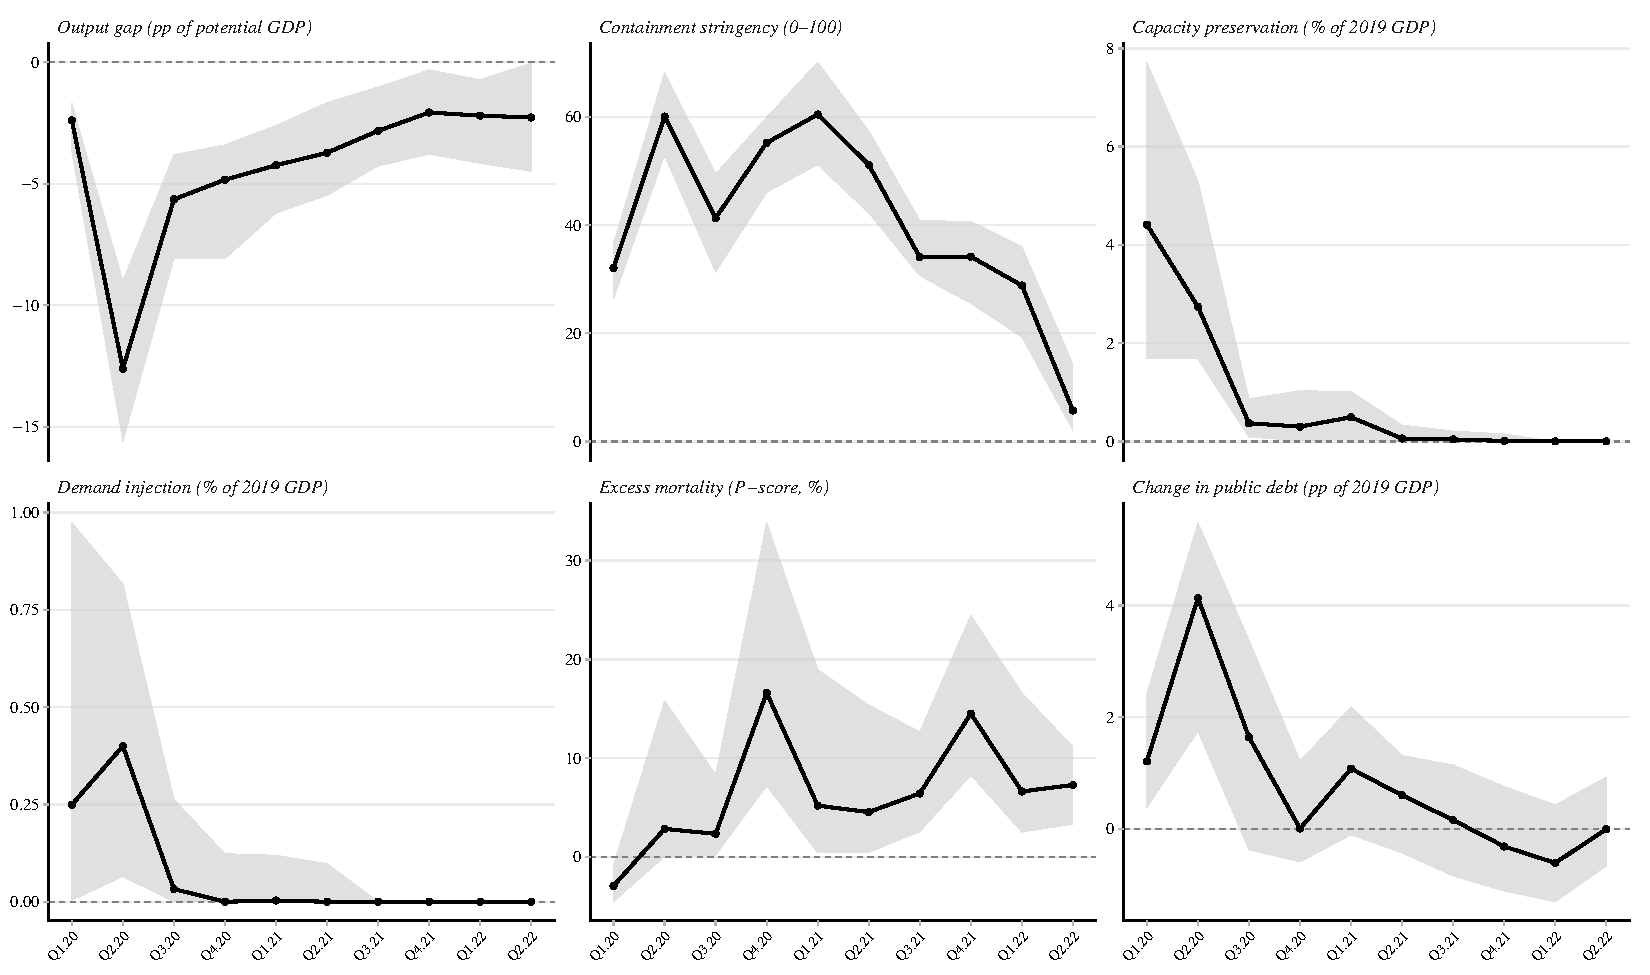
\includegraphics[width=0.6\textwidth]{fig_ts_key_variables_v2.pdf}
    \caption{OECD Pandemic Trajectories by Quarter}
    \label{fig:trajectories}
    \vspace{4pt}
    \parbox{\textwidth}{\footnotesize \textit{Notes:} Each panel plots the cross-country median (solid line) and interquartile range (P25--P75, shaded band) across 38 OECD countries per quarter, Q1\,2020--Q2\,2022. All variables are quarterly country-level observations as defined in Section~\ref{subsec:data}. The narrow interquartile range for containment stringency relative to the wide bands for capacity preservation and demand injection reflects the compositional heterogeneity that drives identification.}
\end{figure}

\subsection{Results}
\label{sec:results_empirical}


\begin{table}[H]
\centering
\caption{Main Results: Output Gap Equation}
\label{tab:main_results}
\scriptsize
\renewcommand{\arraystretch}{1.2}
\begin{tabular}{@{} l c c c @{}}
\toprule
 & (1) & (2) & (3) \\
 & Pooled OLS & Country FE & Country + Quarter FE \\
\midrule
\multicolumn{4}{@{}l}{\textit{Persistence channels:}} \\[2pt]
$y_{i,k-1}$ (baseline $\rho_y$)
  & $0.767$***  & $0.174$**   & $0.311$*** \\
  & (0.080)     & (0.067)     & (0.085) \\[4pt]
$S_{ik} \times y_{i,k-1}$ (lockdown $\psi$)
  & $-0.004$    & $0.000$     & $0.002$* \\
  & (0.002)     & (0.002)     & (0.001) \\[4pt]
$F^{CP}_{i,k-2} \times y_{i,k-1}$ (CP $-\eta_p$)
  & $-0.024$*** & $-0.005$    & $-0.011$*** \\
  & (0.007)     & (0.003)     & (0.003) \\[4pt]
\multicolumn{4}{@{}l}{\textit{Level channels:}} \\[2pt]
$S_{ik}$ (containment $\alpha_S$)
  & $-0.092$*** & $-0.116$*** & $-0.034$*** \\
  & (0.019)     & (0.013)     & (0.012) \\[4pt]
$F^{DI}_{i,k-2}$ (DI $\alpha_{DI}$)
  & $0.999$***  & $0.663$***  & $0.185$ \\
  & (0.198)     & (0.109)     & (0.122) \\[4pt]
$d_{ik}$ (fear $\beta_d$)
  & $0.003$     & $0.014$     & $-0.021$** \\
  & (0.016)     & (0.015)     & (0.008) \\[4pt]
\midrule
Country FE       &            & \checkmark & \checkmark \\
Quarter FE       &            &            & \checkmark \\
Observations     & 380        & 380        & 380 \\
$R^2$            & 0.454      & 0.628      &            \\
Within $R^2$     &            &            & 0.281 \\
\bottomrule
\end{tabular}
\vspace{4pt}
\parbox{\textwidth}{\scriptsize\textit{Notes:} Dependent variable: output gap $y_{ik}$ (percentage points of potential GDP). Sample: 38 OECD countries over Q1\,2020--Q2\,2022 ($t \geq 5$, ten quarters per country). All columns use identical regressors; columns differ only in the fixed-effects structure. Standard errors clustered at the country level in parentheses, with small-sample adjustment. The progression across columns illustrates the identification strategy. The pooled OLS estimate of $\eta_p$ ($-0.024$) is inflated by cross-country confounding between fiscal composition and country-specific recession depth. Country fixed effects absorb this confounding, and the coefficient collapses to $-0.005$ (insignificant), reflecting the loss of identification without temporal variation. Quarter fixed effects restore identification from within-country variation across quarters, yielding $\eta_p = -0.011$ ($p < 0.001$). The lockdown amplification parameter $\psi$ follows a parallel pattern: negative in pooled OLS (sign reversal from omitted-variable bias), zero under country FE alone, and correctly signed and significant under the two-way specification. The level of $F^{CP}$ is omitted because the theoretical framework predicts no contemporaneous level effect; a specification including $F^{CP}$ as a level control is reported in Section~\ref{subsec:robustness}. * $p<0.1$, ** $p<0.05$, *** $p<0.01$.}
\end{table}

\begin{table}[H]
\centering
\caption{Robustness: Persistence Channel $\eta_p$ across Specifications}
\label{tab:robustness_etap}
\scriptsize
\renewcommand{\arraystretch}{1.15}
\begin{tabular}{@{} l r r r c r @{}}
\toprule
Specification & $\hat{\eta}_p$ & SE & $p$-value & & $N$ \\
\midrule
\multicolumn{6}{@{}l}{\textit{Panel A: Baseline \& outlier exclusion}} \\[2pt]
Baseline                        & $-0.011$ & (0.003) & 0.000 & *** & 380 \\
No IRL                          & $-0.011$ & (0.003) & 0.000 & *** & 370 \\
No TUR                          & $-0.011$ & (0.003) & 0.000 & *** & 370 \\
No IRL + TUR                    & $-0.010$ & (0.003) & 0.001 & *** & 360 \\[4pt]
\multicolumn{6}{@{}l}{\textit{Panel B: Alternative controls \& measures}} \\[2pt]
$S^{\max}_{ik}$ instead of $S^{\text{mean}}_{ik}$
                                & $-0.011$ & (0.003) & 0.000 & *** & 380 \\
+ Vaccination rate              & $-0.012$ & (0.003) & 0.000 & *** & 380 \\
Fear: $\theta_{ik}$ (infection prevalence)
                                & $-0.011$ & (0.003) & 0.000 & *** & 380 \\
Fear: $\bar{p}_{ik}$ (avg.\ P-score)
                                & $-0.011$ & (0.003) & 0.000 & *** & 380 \\
+ Health expenditure ($F^H$)    & $-0.012$ & (0.003) & 0.000 & *** & 380 \\
+ ICU occupancy                 & $-0.009$ & (0.003) & 0.010 & **  & 194 \\
+ $F^{CP}_{i,k-2}$ level        & $-0.021$ & (0.006) & 0.001 & *** & 380 \\[4pt]
\multicolumn{6}{@{}l}{\textit{Panel C: Sample variations}} \\[2pt]
Extended (Q4.2019--Q4.2022)     & $-0.013$ & (0.003) & 0.000 & *** & 456 \\
Only 2020 (Q4.2019--Q4.2020)   & $-0.008$ & (0.003) & 0.003 & *** & 152 \\
Shorter (Q1.2020--Q1.2022)     & $-0.010$ & (0.003) & 0.001 & *** & 342 \\[4pt]
\multicolumn{6}{@{}l}{\textit{Panel D: Sample splits}} \\[2pt]
High stringency                 & $-0.015$ & (0.004) & 0.001 & *** & 190 \\
Low stringency                  & $+0.001$ & (0.008) & 0.931 &     & 190 \\
High income                     & $-0.009$ & (0.003) & 0.007 & *** & 200 \\
Low income                      & $-0.017$ & (0.005) & 0.001 & *** & 200 \\
High social safety nets         & $-0.010$ & (0.003) & 0.004 & *** & 190 \\
Low social safety nets          & $-0.020$ & (0.010) & 0.067 & *   & 190 \\
\midrule
\multicolumn{6}{@{}l}{Significant at 1\%: 17/20 \quad at 5\%: 18/20 \quad at 10\%: 19/20} \\
\bottomrule
\end{tabular}
\vspace{4pt}
\parbox{\textwidth}{\scriptsize\textit{Notes:} Each row re-estimates the full V3 specification
$y_{ik} = \mu_i + \varepsilon_k + \rho\, y_{i,k-1} + \psi\, S_{ik} y_{i,k-1}
- \eta_p\, F^{CP}_{i,k-2} y_{i,k-1} + \alpha_S\, S_{ik}
+ \alpha_{DI}\, F^{DI}_{i,k-2} + \beta_d\, d_{ik} + u_{ik}$
with the modification indicated. Standard errors clustered by country.
The ``$+F^{CP}$ level'' row adds $F^{CP}_{i,k-2}$ as a level regressor;
$\hat{\eta}_p$ doubles because the level absorbs part of the mean,
leaving the interaction to capture steeper within-variation.
The low-stringency subsample shows $\eta_p \approx 0$, consistent with
the model prediction that the persistence channel requires an active
lockdown shock: where $S$ is low, output gap persistence is small and
$F^{CP}$ has no margin to preserve against.
* $p<0.1$, ** $p<0.05$, *** $p<0.01$.}
\end{table}


\begin{table}[H]
\centering
\caption{Robustness: Demand Injection $\alpha_{DI}$ across Specifications}
\label{tab:robustness_di}
\scriptsize
\renewcommand{\arraystretch}{1.15}
\begin{tabular}{@{} l r r r c r @{}}
\toprule
Specification & $\hat{\alpha}_{DI}$ & SE & $p$-value & & $N$ \\
\midrule
\multicolumn{6}{@{}l}{\textit{Panel A: Baseline \& outlier exclusion}} \\[2pt]
Baseline                        & $+0.185$ & (0.122) & 0.138 &     & 380 \\
No IRL                          & $+0.138$ & (0.128) & 0.287 &     & 370 \\
No TUR                          & $+0.199$ & (0.118) & 0.102 &     & 370 \\
No IRL + TUR                    & $+0.148$ & (0.125) & 0.246 &     & 360 \\[4pt]
\multicolumn{6}{@{}l}{\textit{Panel B: Alternative controls \& measures}} \\[2pt]
$S^{\max}_{ik}$ instead of $S^{\text{mean}}_{ik}$
                                & $+0.222$ & (0.120) & 0.074 & *   & 380 \\
+ Vaccination rate              & $+0.184$ & (0.116) & 0.123 &     & 380 \\
Fear: $\theta_{ik}$ (infection prevalence)
                                & $+0.206$ & (0.127) & 0.114 &     & 380 \\
Fear: $\bar{p}_{ik}$ (avg.\ P-score)
                                & $+0.186$ & (0.122) & 0.137 &     & 380 \\
+ Health expenditure ($F^H$)    & $+0.189$ & (0.124) & 0.138 &     & 380 \\
+ ICU occupancy                 & $+0.136$ & (0.189) & 0.480 &     & 194 \\
+ $F^{CP}_{i,k-2}$ level        & $+0.215$ & (0.115) & 0.070 & *   & 380 \\[4pt]
\multicolumn{6}{@{}l}{\textit{Panel C: Lag structure}} \\[2pt]
$F^{DI}_{i,k-1}$ (lag 1)       & $-0.077$ & (0.108) & 0.478 &     & 380 \\
$F^{DI}_{i,k-3}$ (lag 3)       & $+0.021$ & (0.134) & 0.876 &     & 380 \\[4pt]
\multicolumn{6}{@{}l}{\textit{Panel D: Sample variations}} \\[2pt]
Extended (Q4.2019--Q4.2022)     & $+0.153$ & (0.130) & 0.244 &     & 456 \\
Only 2020 (Q4.2019--Q4.2020)   & $+0.060$ & (0.248) & 0.812 &     & 152 \\
Shorter (Q1.2020--Q1.2022)     & $+0.200$ & (0.125) & 0.119 &     & 342 \\[4pt]
\multicolumn{6}{@{}l}{\textit{Panel E: Sample splits}} \\[2pt]
High stringency                 & $+0.221$ & (0.128) & 0.102 &     & 190 \\
Low stringency                  & $+0.125$ & (0.103) & 0.243 &     & 190 \\
High income                     & $+0.119$ & (0.157) & 0.455 &     & 200 \\
Low income                      & $+0.180$ & (0.158) & 0.267 &     & 200 \\
High social safety nets         & $-0.082$ & (0.244) & 0.739 &     & 190 \\
Low social safety nets          & $+0.269$ & (0.133) & 0.058 & *   & 190 \\
\midrule
\multicolumn{6}{@{}l}{Significant at 1\%: 0/22 \quad at 5\%: 0/22 \quad at 10\%: 3/22} \\
\bottomrule
\end{tabular}
\vspace{4pt}
\parbox{\textwidth}{\scriptsize\textit{Notes:} Each row re-estimates the full V3 specification with the modification indicated. $\alpha_{DI}$ is the coefficient on $F^{DI}_{i,k-2}$ (lag~2 unless otherwise noted). Standard errors clustered by country. The coefficient is consistently positive ($+0.12$ to $+0.27$) across 19 of 22 specifications but rarely reaches conventional significance, reflecting (i)~58\% zero observations in $F^{DI}$, (ii)~the two-quarter lag reducing effective variation, and (iii)~small magnitudes (mean $0.26$~pp GDP vs $1.31$ for $F^{CP}$). Panel~C confirms the lag~2 timing: lag~1 is negative and insignificant (too early), lag~3 attenuates to zero (too late), consistent with a disbursement-to-spending delay of approximately two quarters. The low-social-safety-net subsample --- dominated by countries that relied more heavily on direct transfers (USA, CAN, CHL, AUS) --- yields the strongest and only marginally significant effect ($+0.269$, $p = 0.058$). * $p<0.1$, ** $p<0.05$, *** $p<0.01$.}
\end{table}

% =============================================================================
%  ROBUSTNESS TABLE: alpha_S (Stringency)
% =============================================================================
\begin{table}[H]
\centering
\caption{Robustness: Stringency $\alpha_S$ across Specifications}
\label{tab:robustness_alphaS}
\scriptsize
\renewcommand{\arraystretch}{1.15}
\begin{tabular}{@{} l r r r c r @{}}
\toprule
Specification & $\hat{\alpha}_S$ & SE & $p$-value & & $N$ \\
\midrule
\multicolumn{6}{@{}l}{\textit{Panel A: Baseline \& outlier exclusion}} \\[2pt]
Baseline                        & $-0.034$ & (0.012) & 0.006 & *** & 380 \\
No IRL                          & $-0.032$ & (0.015) & 0.040 & **  & 370 \\
No TUR                          & $-0.031$ & (0.012) & 0.016 & **  & 370 \\
No IRL + TUR                    & $-0.025$ & (0.016) & 0.123 &     & 360 \\[4pt]
\multicolumn{6}{@{}l}{\textit{Panel B: Alternative controls \& measures}} \\[2pt]
$S^{\max}_{ik}$                 & $-0.024$ & (0.009) & 0.013 & **  & 380 \\
+ Vaccination rate              & $-0.036$ & (0.012) & 0.006 & *** & 380 \\
Fear: $\theta_{ik}$             & $-0.037$ & (0.012) & 0.003 & *** & 380 \\
Fear: $\bar{p}_{ik}$            & $-0.034$ & (0.012) & 0.006 & *** & 380 \\
+ Health expenditure ($F^H$)    & $-0.034$ & (0.012) & 0.006 & *** & 380 \\
+ ICU occupancy                 & $-0.028$ & (0.022) & 0.210 &     & 194 \\
+ $F^{CP}_{i,k-2}$ level        & $-0.033$ & (0.012) & 0.008 & *** & 380 \\[4pt]
\multicolumn{6}{@{}l}{\textit{Panel C: Sample variations}} \\[2pt]
Extended (Q4.2019--Q4.2022)     & $-0.033$ & (0.010) & 0.001 & *** & 456 \\
Only 2020                       & $-0.070$ & (0.021) & 0.002 & *** & 152 \\
Shorter (Q1.2020--Q1.2022)     & $-0.033$ & (0.014) & 0.019 & **  & 342 \\[4pt]
\multicolumn{6}{@{}l}{\textit{Panel D: Sample splits}} \\[2pt]
High stringency                 & $-0.031$ & (0.018) & 0.113 &     & 190 \\
Low stringency                  & $-0.024$ & (0.018) & 0.188 &     & 190 \\
High income                     & $-0.035$ & (0.015) & 0.026 & **  & 200 \\
Low income                      & $-0.031$ & (0.019) & 0.118 &     & 200 \\
High social safety nets         & $-0.001$ & (0.023) & 0.977 &     & 190 \\
Low social safety nets          & $-0.046$ & (0.013) & 0.003 & *** & 190 \\
\midrule
\multicolumn{6}{@{}l}{Significant at 1\%: 8/20 \quad at 5\%: 13/20 \quad at 10\%: 13/20} \\
\bottomrule
\end{tabular}
\vspace{4pt}
\parbox{\textwidth}{\scriptsize\textit{Notes:} Each row re-estimates the full V3 specification with the modification indicated. $\alpha_S$ is the direct effect of the stringency index $S_{ik}$ on the output gap. Standard errors clustered by country. The coefficient is consistently negative ($-0.024$ to $-0.070$) and significant in 13 of 20 specifications. The ``$S^{\max}$'' row uses the within-quarter maximum instead of the mean. The coefficient roughly doubles in the 2020-only subsample ($-0.070$), consistent with stringency having its strongest bite during the initial lockdown waves. The high-social-safety-net subsample shows $\alpha_S \approx 0$, suggesting that generous automatic stabilizers offset the direct output cost of lockdowns. * $p<0.1$, ** $p<0.05$, *** $p<0.01$.}
\end{table}


% =============================================================================
%  ROBUSTNESS TABLE: rho_y (Persistence)
% =============================================================================
\begin{table}[H]
\centering
\caption{Robustness: Persistence $\rho_y$ across Specifications}
\label{tab:robustness_rhoy}
\scriptsize
\renewcommand{\arraystretch}{1.15}
\begin{tabular}{@{} l r r r c r @{}}
\toprule
Specification & $\hat{\rho}_y$ & SE & $p$-value & & $N$ \\
\midrule
\multicolumn{6}{@{}l}{\textit{Panel A: Baseline \& outlier exclusion}} \\[2pt]
Baseline                        & $+0.311$ & (0.085) & 0.001 & *** & 380 \\
No IRL                          & $+0.270$ & (0.115) & 0.024 & **  & 370 \\
No TUR                          & $+0.273$ & (0.094) & 0.006 & *** & 370 \\
No IRL + TUR                    & $+0.198$ & (0.122) & 0.114 &     & 360 \\[4pt]
\multicolumn{6}{@{}l}{\textit{Panel B: Alternative controls \& measures}} \\[2pt]
$S^{\max}_{ik}$                 & $+0.324$ & (0.090) & 0.001 & *** & 380 \\
+ Vaccination rate              & $+0.310$ & (0.080) & 0.000 & *** & 380 \\
Fear: $\theta_{ik}$             & $+0.276$ & (0.091) & 0.004 & *** & 380 \\
Fear: $\bar{p}_{ik}$            & $+0.309$ & (0.085) & 0.001 & *** & 380 \\
+ Health expenditure ($F^H$)    & $+0.323$ & (0.089) & 0.001 & *** & 380 \\
+ ICU occupancy                 & $+0.026$ & (0.177) & 0.884 &     & 194 \\
+ $F^{CP}_{i,k-2}$ level        & $+0.329$ & (0.087) & 0.001 & *** & 380 \\[4pt]
\multicolumn{6}{@{}l}{\textit{Panel C: Sample variations}} \\[2pt]
Extended (Q4.2019--Q4.2022)     & $+0.521$ & (0.073) & 0.000 & *** & 456 \\
Only 2020                       & $-0.021$ & (0.107) & 0.843 &     & 152 \\
Shorter (Q1.2020--Q1.2022)     & $+0.169$ & (0.091) & 0.073 & *   & 342 \\[4pt]
\multicolumn{6}{@{}l}{\textit{Panel D: Sample splits}} \\[2pt]
High stringency                 & $+0.418$ & (0.100) & 0.001 & *** & 190 \\
Low stringency                  & $-0.012$ & (0.128) & 0.928 &     & 190 \\
High income                     & $+0.290$ & (0.136) & 0.046 & **  & 200 \\
Low income                      & $+0.422$ & (0.122) & 0.003 & *** & 200 \\
High social safety nets         & $+0.182$ & (0.217) & 0.412 &     & 190 \\
Low social safety nets          & $+0.385$ & (0.085) & 0.000 & *** & 190 \\
\midrule
\multicolumn{6}{@{}l}{Significant at 1\%: 12/20 \quad at 5\%: 14/20 \quad at 10\%: 15/20} \\
\bottomrule
\end{tabular}
\vspace{4pt}
\parbox{\textwidth}{\scriptsize\textit{Notes:} Each row re-estimates the full V3 specification with the modification indicated. $\rho_y$ is the baseline persistence of the output gap (at $S = 0$ and $F^{CP} = 0$). Standard errors clustered by country. The coefficient is positive and significant in 15 of 20 specifications, with a baseline estimate of $0.311$. Persistence rises in the extended sample ($0.521$) as recovery quarters strengthen the AR(1) pattern. The 2020-only subsample shows $\rho_y \approx 0$: with only four pandemic quarters, the output gap path is dominated by the lockdown shock and rebound rather than autoregressive dynamics. Low-stringency countries also show zero persistence, consistent with the model: where lockdowns were mild, output gaps were small and transitory. * $p<0.1$, ** $p<0.05$, *** $p<0.01$.}
\end{table}


% =============================================================================
%  ROBUSTNESS TABLE: psi (Lockdown amplification)
% =============================================================================
\begin{table}[H]
\centering
\caption{Robustness: Lockdown Amplification $\psi$ across Specifications}
\label{tab:robustness_psi}
\scriptsize
\renewcommand{\arraystretch}{1.15}
\begin{tabular}{@{} l r r r c r @{}}
\toprule
Specification & $\hat{\psi}$ & SE & $p$-value & & $N$ \\
\midrule
\multicolumn{6}{@{}l}{\textit{Panel A: Baseline \& outlier exclusion}} \\[2pt]
Baseline                        & $+0.002$ & (0.001) & 0.075 & *   & 380 \\
No IRL                          & $+0.003$ & (0.002) & 0.093 & *   & 370 \\
No TUR                          & $+0.003$ & (0.001) & 0.073 & *   & 370 \\
No IRL + TUR                    & $+0.004$ & (0.002) & 0.053 & *   & 360 \\[4pt]
\multicolumn{6}{@{}l}{\textit{Panel B: Alternative controls \& measures}} \\[2pt]
$S^{\max}_{ik}$                 & $+0.002$ & (0.001) & 0.097 & *   & 380 \\
+ Vaccination rate              & $+0.002$ & (0.001) & 0.052 & *   & 380 \\
Fear: $\theta_{ik}$             & $+0.003$ & (0.001) & 0.028 & **  & 380 \\
Fear: $\bar{p}_{ik}$            & $+0.002$ & (0.001) & 0.068 & *   & 380 \\
+ Health expenditure ($F^H$)    & $+0.002$ & (0.001) & 0.097 & *   & 380 \\
+ ICU occupancy                 & $+0.005$ & (0.002) & 0.044 & **  & 194 \\
+ $F^{CP}_{i,k-2}$ level        & $+0.002$ & (0.001) & 0.055 & *   & 380 \\[4pt]
\multicolumn{6}{@{}l}{\textit{Panel C: Sample variations}} \\[2pt]
Extended (Q4.2019--Q4.2022)     & $+0.001$ & (0.001) & 0.613 &     & 456 \\
Only 2020                       & $+0.002$ & (0.002) & 0.329 &     & 152 \\
Shorter (Q1.2020--Q1.2022)     & $+0.004$ & (0.001) & 0.009 & *** & 342 \\[4pt]
\multicolumn{6}{@{}l}{\textit{Panel D: Sample splits}} \\[2pt]
High stringency                 & $+0.002$ & (0.001) & 0.194 &     & 190 \\
Low stringency                  & $+0.004$ & (0.003) & 0.145 &     & 190 \\
High income                     & $+0.002$ & (0.002) & 0.319 &     & 200 \\
Low income                      & $+0.001$ & (0.002) & 0.467 &     & 200 \\
High social safety nets         & $+0.005$ & (0.003) & 0.122 &     & 190 \\
Low social safety nets          & $+0.001$ & (0.001) & 0.568 &     & 190 \\
\midrule
\multicolumn{6}{@{}l}{Significant at 1\%: 1/20 \quad at 5\%: 3/20 \quad at 10\%: 12/20} \\
\bottomrule
\end{tabular}
\vspace{4pt}
\parbox{\textwidth}{\scriptsize\textit{Notes:} Each row re-estimates the full V3 specification with the modification indicated. $\psi$ is the lockdown amplification parameter from the interaction $S_{ik} \times y_{i,k-1}$: higher stringency increases the persistence of the output gap. Standard errors clustered by country. The coefficient is consistently positive across all 20 specifications ($+0.001$ to $+0.005$) and significant at 10\% in 12 of 20. The effect is identified most precisely in the core pandemic window (Q1.2020--Q1.2022: $\psi = 0.004$, $p < 0.01$) and attenuates in the extended sample where post-pandemic quarters dilute the lockdown-persistence nexus. Subsample splits lack power due to halved sample size, but all point estimates remain positive. * $p<0.1$, ** $p<0.05$, *** $p<0.01$.}
\end{table}


% =============================================================================
%  ROBUSTNESS TABLE: beta_d (Fear term)
% =============================================================================
\begin{table}[H]
\centering
\caption{Robustness: Fear Term $\beta_d$ across Specifications}
\label{tab:robustness_betad}
\scriptsize
\renewcommand{\arraystretch}{1.15}
\begin{tabular}{@{} l r r r c r @{}}
\toprule
Specification & $\hat{\beta}_d$ & SE & $p$-value & & $N$ \\
\midrule
\multicolumn{6}{@{}l}{\textit{Panel A: Baseline \& outlier exclusion}} \\[2pt]
Baseline                        & $-0.021$ & (0.008) & 0.017 & **  & 380 \\
No IRL                          & $-0.022$ & (0.008) & 0.012 & **  & 370 \\
No TUR                          & $-0.024$ & (0.008) & 0.006 & *** & 370 \\
No IRL + TUR                    & $-0.024$ & (0.008) & 0.006 & *** & 360 \\[4pt]
\multicolumn{6}{@{}l}{\textit{Panel B: Alternative controls \& measures}} \\[2pt]
$S^{\max}_{ik}$                 & $-0.023$ & (0.009) & 0.015 & **  & 380 \\
+ Vaccination rate              & $-0.020$ & (0.008) & 0.017 & **  & 380 \\
Fear: $\theta_{ik}$             & $-0.008$ & (0.094) & 0.931 &     & 380 \\
Fear: $\bar{p}_{ik}$            & $-0.018$ & (0.008) & 0.023 & **  & 380 \\
+ Health expenditure ($F^H$)    & $-0.021$ & (0.008) & 0.018 & **  & 380 \\
+ ICU occupancy                 & $-0.037$ & (0.023) & 0.124 &     & 194 \\
+ $F^{CP}_{i,k-2}$ level        & $-0.020$ & (0.008) & 0.021 & **  & 380 \\[4pt]
\multicolumn{6}{@{}l}{\textit{Panel C: Sample variations}} \\[2pt]
Extended (Q4.2019--Q4.2022)     & $-0.023$ & (0.008) & 0.006 & *** & 456 \\
Only 2020                       & $-0.016$ & (0.018) & 0.382 &     & 152 \\
Shorter (Q1.2020--Q1.2022)     & $-0.020$ & (0.009) & 0.038 & **  & 342 \\[4pt]
\multicolumn{6}{@{}l}{\textit{Panel D: Sample splits}} \\[2pt]
High stringency                 & $-0.034$ & (0.014) & 0.025 & **  & 190 \\
Low stringency                  & $-0.007$ & (0.012) & 0.578 &     & 190 \\
High income                     & $-0.038$ & (0.026) & 0.165 &     & 200 \\
Low income                      & $-0.023$ & (0.008) & 0.006 & *** & 200 \\
High social safety nets         & $-0.043$ & (0.022) & 0.066 & *   & 190 \\
Low social safety nets          & $-0.012$ & (0.009) & 0.182 &     & 190 \\
\midrule
\multicolumn{6}{@{}l}{Significant at 1\%: 4/20 \quad at 5\%: 12/20 \quad at 10\%: 13/20} \\
\bottomrule
\end{tabular}
\vspace{4pt}
\parbox{\textwidth}{\scriptsize\textit{Notes:} Each row re-estimates the full V3 specification with the modification indicated. $\beta_d$ captures the voluntary demand reduction from infection fear (P-score excess mortality). Standard errors clustered by country. The coefficient is negative and significant in 13 of 20 specifications. The ``$\theta_{ik}$'' row replaces the P-score with infection prevalence --- the coefficient collapses because $\theta$ is collinear with the quarter FE (common pandemic waves). The ``$\bar{p}_{ik}$'' row uses the historical-average rather than projection-based P-score, with similar results. The fear effect is concentrated in high-stringency and high-social-safety-net countries, where lockdowns made mortality salience a binding constraint on consumer behaviour beyond the mechanical lockdown effect. * $p<0.1$, ** $p<0.05$, *** $p<0.01$.}
\end{table}


\begin{table}[H]
\centering
\caption{Main Results: Debt Equation}
\label{tab:debt_main}
\scriptsize
\renewcommand{\arraystretch}{1.2}
\begin{tabular}{@{} l c c c c c @{}}
\toprule
 & (1) & (2) & (3) & (4) & (5) \\
 & OLS & Country FE & \multicolumn{3}{c}{Country FE --- CP decomposition} \\
 \cmidrule(lr){4-6}
 &     & Pooled & Raw & Adj.\ 35\% & Three-way \\
\midrule
$y_{ik}$ [$-\gamma_y$]
  & $-0.147$*** & $-0.219$*** & $-0.215$*** & $-0.215$*** & $-0.210$*** \\
  & (0.029)     & (0.036)     & (0.036)     & (0.036)     & (0.037) \\[4pt]
$F^{CP}_{ik}$ (pooled) [$\kappa^{CP}$]
  & $0.186$***  & $0.167$**   &             &             &  \\
  & (0.049)     & (0.048)     &             &             &  \\[4pt]
$F^{CP}$ above-the-line [$\kappa^{\text{above}}$]
  &             &             & $0.401$*    & $0.401$*    & $0.423$* \\
  &             &             & (0.176)     & (0.176)     & (0.174) \\[4pt]
$F^{CP}$ below-the-line [$\kappa^{\text{below}}$]
  &             &             & $0.112$*    &             &  \\
  &             &             & (0.045)     &             &  \\[4pt]
$F^{CP}$ below-the-line (adj.) [$\kappa^{\text{below}}$]
  &             &             &             & $0.321$*    &  \\
  &             &             &             & (0.127)     &  \\[4pt]
$F^{CP}$ loans [$\kappa^{\text{loans}}$]
  &             &             &             &             & $0.352$*** \\
  &             &             &             &             & (0.083) \\[4pt]
$F^{CP}$ guarantees (adj.) [$\kappa^{\text{guar}}$]
  &             &             &             &             & $0.095$ \\
  &             &             &             &             & (0.164) \\[4pt]
$F^{DI}_{i,k}$ [$\kappa^{DI}$]
  & $0.375$    & $0.161$     & $0.215$     & $0.215$     & $0.181$ \\
  & (0.293)     & (0.281)     & (0.283)     & (0.283)     & (0.282) \\[4pt]
\midrule
Country FE           &       & \checkmark & \checkmark & \checkmark & \checkmark \\
Guarantee adjustment & ---   & ---        & No         & 35\%       & 35\% \\
Observations         & 380   & 380        & 380        & 380        & 380 \\
Within $R^2$         &       & 0.220      & 0.228      & 0.228      & 0.238 \\
\bottomrule
\end{tabular}
\vspace{4pt}

\parbox{\textwidth}{\scriptsize\textit{Notes:} Dependent variable:
$\Delta b_{ik}$ (quarterly first difference of real public debt, pp of
2019 GDP). 38 OECD countries, Q1\,2020--Q2\,2022 (380 observations).
Standard errors clustered by country in parentheses. All fiscal
variables in \% of 2019 GDP. Column~(1): pooled OLS. Column~(2):
country fixed effects, pooled capacity preservation. Column~(3): CP
disaggregated into above-the-line (wage subsidies, grants) and
below-the-line (loans, guarantees) at face value. Column~(4):
below-the-line adjusted for 35\% guarantee take-up rate
\citep{imf2022fiscalmonitor}. Column~(5): three-way decomposition into
above-the-line, government loans (actual disbursements), and credit
guarantees (contingent liabilities, adjusted at 35\%). Loans are highly
significant ($\hat{\kappa}^{\text{loans}} = 0.35$***, $p < 0.001$)
while guarantees are insignificant ($p = 0.57$), consistent with the
``whatever it takes'' logic: guarantees preserve capacity through
announcement effects but most are never drawn, generating no realized
debt. $F^{DI}$ enters at lag~1. * $p<0.1$, ** $p<0.05$, *** $p<0.01$.}
\end{table}


%5NEXT STEPS
%Fix Identification-> no linear trend anymore
%Do the interpretation, what do I find? DI is nothing (both sphere)
%Total fiscal mal noch hinzu-> schauen ob ich mit CP einen Effekt identifizieren kann und sonst nicht
%MatLab 10 and 9 are the right Version-> See claude for conversation



\section{Optimization}
\subsection{Solution Method}

With all structural parameters either estimated from the panel (Section~\ref{sec:estimation}) or calibrated from the literature (Table~\ref{tab:calibration}), the planner's problem~\eqref{eq:objective1} is solved numerically using an iterative Linear-Quadratic Regulator (iLQR)---a direct shooting method following \citet{li2004iterative} and \citet{bertsekas2017dynamic}. The algorithm alternates between a forward pass that rolls the nonlinear transition system~\eqref{eq:plan_theta}--\eqref{eq:plan_b} forward under a candidate control sequence, and a backward pass that solves a time-varying LQR problem around the resulting trajectory to update the controls. Non-negativity constraints on the controls ($S_k, F^{CP}_k, F^{DI}_k \geq 0$) are enforced through an Augmented Lagrangian scheme. The solver is initialized at each country's observed fiscal trajectory, and convergence is verified by solving from alternative initializations.

The planner's weights $(w_d, w_y, w_b, W_b)$ and control penalties $(r_S, r_{CP}, r_{DI})$ are not estimated but selected to reflect the preferences revealed by observed policy: the weights are calibrated such that the unconstrained aggregate optimum reproduces the OECD-average trajectory of output and debt over Q1\,2020--Q2\,2022. This revealed-preference calibration serves as the benchmark against which country-specific counterfactuals are evaluated. For the counterfactual exercises, $\{S_k\}$ is fixed at each country's empirically observed trajectory and the induced epidemiological states $\{\theta_k, d_k\}$ enter as predetermined inputs, so that the optimization reduces to the fiscal controls $\{F^{CP}_k, F^{DI}_k\}$ under the same preference weights.

%APROACH hier
\subsection{Calibration}

\noindent The transition system~\eqref{eq:plan_theta}--\eqref{eq:plan_b} contains two sets of structural parameters. The first set---governing epidemiological dynamics and the macroeconomic environment---is calibrated from the existing literature. The second set---governing the transmission of disaggregated fiscal instruments to output and debt---is estimated from the panel data. Table~\ref{tab:calibration} reports the calibrated parameters with sources; Table~\ref{tab:estimated} reports the estimated parameters with standard errors. A complete list of all variables and parameters is provided in Table~\ref{tab:full_parameter} in the Appendix.

\begin{table}[H]
\centering
\caption{Calibrated Parameters\protect\footnotemark}
\label{tab:calibration}
\scriptsize
\begin{tabular}{@{} c l c l @{}}
\toprule
\textbf{Parameter} & \textbf{Description} & \textbf{Value} & \textbf{Source} \\
\midrule
$\rho_\theta$ & Eff.\ reproduction rate (quarterly)
    & 1.25--1.70
    & \citet{dhungel2022, liu2021rocklov} \\
$\delta_\theta$ & Infection fatality rate
    & 0.003--0.020
    & \citet{IHME2022lancet, Levin2020} \\
$\phi_S$ & NPI suppression effectiveness
    & 0.4--0.7
    & \citet{brauner2021inferring, haug2020ranking} \\
$r$ & Real interest rate (quarterly)
    & $\approx 0.001$
    & \citet{OECD2022borrowing} \\
$\beta$ & Discount factor (quarterly)
    & 0.99
    & Standard \\
$c_H$ & Health expenditure per \% infection
    & 0.02
    & \citet{imf2022fiscalmonitor, OECD2023health} \\
\bottomrule
\end{tabular}
\end{table}
\footnotetext{The epidemiological parameters $\rho_\theta$ and $\delta_\theta$ vary across pandemic waves; the ranges reported here span from the second wave (late 2020) through Omicron (Q4\,2021). Wave-specific values and their sources are reported in Table~\ref{tab:full_parameter} in the Appendix.}

\begin{table}[H]
\centering
\caption{Estimated Structural Parameters}
\label{tab:estimated}
\scriptsize
\renewcommand{\arraystretch}{1.2}
\begin{tabular}{@{} c l c c @{}}
\toprule
\textbf{Parameter} & \textbf{Description} & \textbf{Estimate} & \textbf{Equation} \\
\midrule
\multicolumn{4}{@{}l}{\textit{Output transition}} \\[2pt]
$\rho_y$      & Baseline output persistence
              & $0.311$*** (0.085)  & \eqref{eq:plan_y} \\
$\psi$        & Lockdown amplification of persistence
              & $0.002$*  \;\,(0.001) & \eqref{eq:plan_y} \\
$\eta_p$      & Capacity preservation persistence channel
              & $-0.011$*** (0.003) & \eqref{eq:plan_y} \\
$\alpha_S$    & Direct output cost of containment
              & $-0.034$*** (0.012) & \eqref{eq:plan_y} \\
$\alpha_{DI}$ & Demand injection multiplier (lag 2)
              & $\phantom{-}0.185$ \;\,\;\,(0.122) & \eqref{eq:plan_y} \\
$\beta_d$     & Behavioral response to mortality
              & $-0.021$** \;\,(0.008) & \eqref{eq:plan_y} \\[4pt]
\multicolumn{4}{@{}l}{\textit{Debt transition}} \\[2pt]
$\gamma_y$    & Budget semi-elasticity (automatic stabilizer)
              & $0.210$*** (0.037) & \eqref{eq:plan_b} \\
$\kappa^{\text{above}}$
              & Above-the-line CP cost
              & $0.423$*  \;\,(0.174) & \eqref{eq:plan_b} \\
$\kappa^{\text{loans}}$
              & CP loans (actual disbursements)
              & $0.352$*** (0.083) & \eqref{eq:plan_b} \\
$\kappa^{\text{guar}}$
              & CP guarantees (35\% take-up)
              & $0.095$ \;\,\;\,\;\,(0.164) & \eqref{eq:plan_b} \\
$\kappa^{DI}$ & Demand injection fiscal cost
              & $0.181$ \;\,\;\,\;\,(0.282) & \eqref{eq:plan_b} \\
\bottomrule
\end{tabular}
\vspace{4pt}
\parbox{\textwidth}{\scriptsize\textit{Notes:} Output parameters from the two-way fixed effects specification (Table~\ref{tab:main_results}, column 3). Debt parameters from the three-way CP decomposition (Table~\ref{tab:debt_main}, column 5). Standard errors clustered at the country level in parentheses. * $p<0.1$, ** $p<0.05$, *** $p<0.01$.}
\end{table}

The estimated parameters identify the two transmission channels that the theoretical framework distinguishes. On the output side, the persistence coefficient $\eta_p = -0.011$ is highly significant, confirming that capacity preservation reduces the effective persistence of the output gap in proportion to the depth of the recession. The demand injection multiplier $\alpha_{DI} = 0.185$ is positive but not statistically distinguishable from zero, consistent with the prediction that demand stimulus is ineffective when supply is physically constrained. On the debt side, the automatic stabilizer $\gamma_y = 0.210$ lies within the OECD range of 0.35--0.65 reported by \citet{repec:oecd} once scale differences are accounted for, and the CP cost decomposition reveals the expected ordering: above-the-line outlays ($0.42$) exceed loan disbursements ($0.35$), which in turn exceed contingent guarantees ($0.10$, insignificant).

\begin{figure}[H]
    \centering
    
\includegraphics[width=0.8\textwidth]{Files/Validation_cal.pdf}
    \caption{Calibration OECD Average}
    \label{fig:trajectories}
    \vspace{4pt}
\end{figure}
\subsection{Scenarios}
\subsection{Counterfactuals}



\section{Conclusion}

\newpage
\section{Robustness}
\label{subsec:robustness}

% =============================================================================
%  ROBUSTNESS CHECKLIST — derived from Referee Discussion
%  Reference document for structuring the Robustness Section
% =============================================================================

\subsection*{Robustness Checks: Summary of Required Tests}

\begin{enumerate}

% -----------------------------------------------------------------
\item \textbf{Simultaneity of $S$ and $F$ (Referee Q1)}
\begin{itemize}
    \item Within-quarter cross-correlation of $\Delta S$ and $F^{CP}$ /
        $F^{DI}$ at weekly frequency (Figure in Appendix~\ref{app:timing})
    \item Asymmetric lag structure: $F$ responds to $S$, not the reverse
        ($r < 0.05$ at negative lags, $r > 0$ at positive lags)
    \item $F^{CP}$ lead test: $F_{i,k+1}^{CP}$ as placebo regressor ---
        expected insignificant
\end{itemize}

\paragraph{Within-quarter timing.}
To verify the temporal ordering of containment and fiscal deployment,
Figure~\ref{fig:crosscorr} reports weekly cross-correlations between changes in
stringency $\Delta S_t$ and fiscal flows $F_t^{CP}$ and $F_t^{DI}$ at lags
$h = -6, \ldots, +6$ weeks. The pattern is strongly asymmetric: at negative lags
(fiscal deployment preceding containment changes), correlations are near zero or
negative ($r < 0.01$ for $h \leq -2$). At lag zero and positive lags (containment
leading fiscal deployment), correlations are positive and persistent, peaking
contemporaneously at $r = 0.19$ for CP and $r = 0.09$ for DI. Granger causality
tests confirm this ordering: $\Delta S$ strongly predicts $F^{CP}$ ($F = 40.7$,
$p < 0.0001$) and $F^{DI}$ ($F = 6.5$, $p < 0.0001$), while $F^{DI}$ does not
predict $\Delta S$ ($F = 0.28$, $p = 0.89$). The reverse direction $F^{CP} \to
\Delta S$ shows some statistical significance ($F = 6.8$, $p < 0.0001$),
consistent with governments announcing lockdown measures and fiscal support
packages simultaneously---this does not threaten identification, which relies on
the orthogonality of fiscal \textit{composition} to containment intensity, not on
the absence of any temporal association between aggregate fiscal deployment and
lockdown decisions.


\begin{figure}[H]
    \centering
    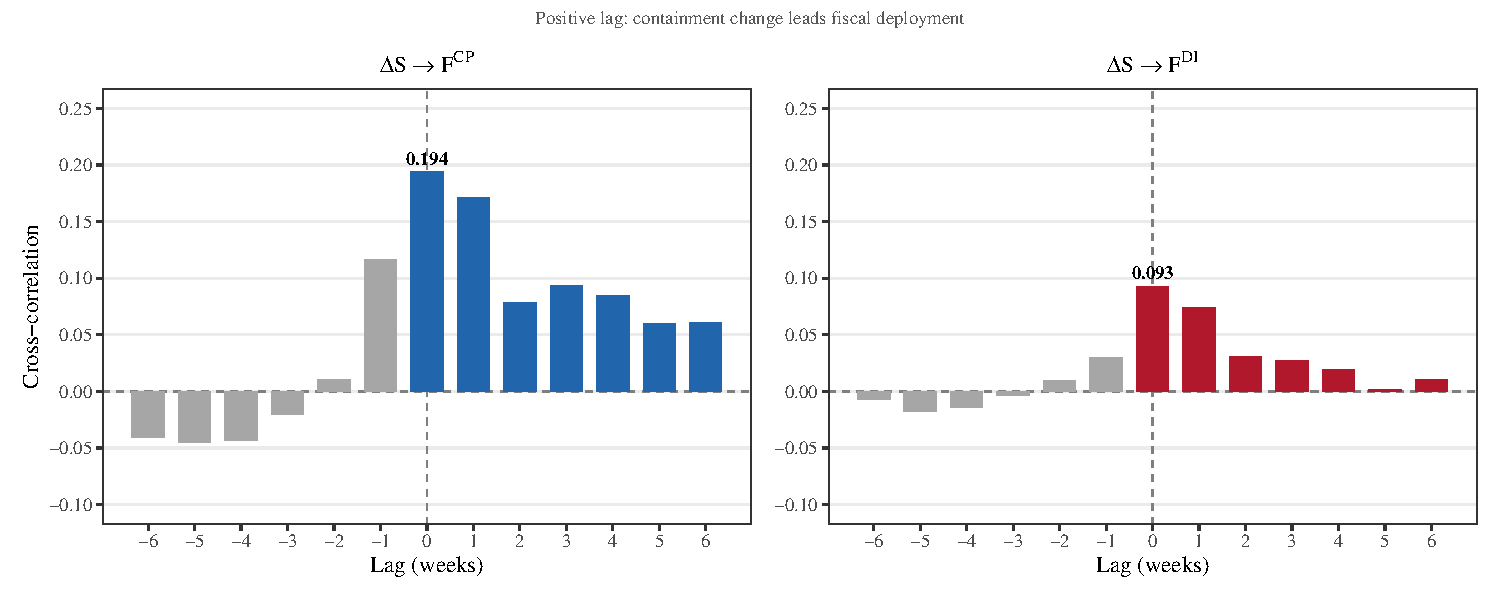
\includegraphics[width=\textwidth]{fig_crosscorr_weekly.pdf}
    \caption{Pandemic Dynamics: Infection Prevalence, Excess Mortality, 
    and Containment}
    \label{fig:planing_horizon}
\end{figure}

% -----------------------------------------------------------------
\item \textbf{Fear Term Specification (Referee Q3)}
\begin{itemize}
    \item Specification without $d_{ik}$: core coefficients
        $\hat{\psi}$, $\hat{\tilde{\eta}}$ stronger / unchanged
    \item Specification with $\theta_{ik}$ instead of $d_{ik}$
    \item Specification with $p_{avg}$ instead of $p_{proj}$
    \item All three: $\hat{\psi}$, $\hat{\tilde{\eta}}$, $\hat{\alpha}_F^{DI}$
        qualitatively unchanged
    \item Identification argument: $d_{ik} = \delta_\theta \theta_{i,k-1}$
        is predetermined relative to $S_{ik}$ $\to$ not a bad control
\end{itemize}

% -----------------------------------------------------------------
\item \textbf{Persistence Channel $\eta_p$ (Referee Q4)}
\begin{itemize}
    \item Specification without $F^{CP} \times y_{i,k-1}$:
        $\hat{\psi}$ and $\hat{\tilde{\eta}}$ stable
    \item $\hat{\eta}_p$ significant in baseline, fragile to outlier
        exclusion and alternative containment measures
    \item Interpretation: suggestive evidence consistent with the
        structural preservation channel; not load-bearing for main results
    \item Identification: within-country time-variation in
        $F^{CP} \times y_{i,k-1}$; GDP publication delay rules out
        contemporaneous reverse causality from $y_{k-1}$ to $F^{CP}_k$
\end{itemize}

% -----------------------------------------------------------------
\item \textbf{Endogeneity of $y_{ik}$ in Debt Equation (Referee Q5)}
\begin{itemize}
    \item Reduced-form specification excluding $y_{ik}$: estimates total
        debt effect (direct costs $+$ automatic stabilizers combined)
    \item $\hat{\kappa}$ in reduced form lower than in baseline $\to$
        confirms self-financing channel
    \item Direction of bias: inclusion of $y_{ik}$ overstates direct
        fiscal cost $\hat{\kappa}$ $\to$ conservative for the
        self-financing argument
    \item Automatic stabilizer is quasi-mechanical (tax-transfer system),
        not a behavioral channel; reverse causality ($b \to y$) implausible
        at quarterly frequency
\end{itemize}

% -----------------------------------------------------------------
\item \textbf{Sample Horizon (Referee Q6)}
\begin{itemize}
    \item Both equations estimated on $T = 9$ (Q1.2020--Q1.2022,
        main specification)
    \item Both equations estimated on $T = 12$ (Q1.2020--Q4.2022,
        robustness)
    \item Coefficients stable across both horizons
\end{itemize}

% -----------------------------------------------------------------
\item \textbf{DI Lag Selection (Referee Q7)}
\begin{itemize}
    \item All three lag specifications (lag 1, 2, 3) reported in a
        single table
    \item Lag 1: insignificant; Lag 2: significant; Lag 3: insignificant
    \item AIC/BIC comparison if available; otherwise transparent that
        selection is based on statistical significance and theoretical
        priors \citep{Blanchard2002, Ramey2011}
    \item DI $\times$ CP complementarity interaction
        \citep{Guerrieri2022}: $p = 0.022$ --- DI effectiveness
        conditional on CP having preserved supply side
\end{itemize}

\end{enumerate}

% -----------------------------------------------------------------
\subsection*{Additional Robustness Checks (from earlier discussion)}

\begin{enumerate}[resume]

\item \textbf{Standard Error Comparison}
\begin{itemize}
    \item HC1 (baseline), HC3, CRV1, CRV3 (Bell--McCaffrey)
    \item Wild Cluster Bootstrap (Rademacher, $B = 9{,}999$)
    \item Qualitative conclusions unchanged across all SE types
\end{itemize}

\item \textbf{Nickell Bias}
\begin{itemize}
    \item $O(1/T) \approx 11\%$; absolute bias $< 0.007$ at
        $\hat{\rho}_y \approx 0.06$
    \item GMM (Arellano--Bond): $\hat{\psi}$ and $\hat{\tilde{\eta}}$
        quantitatively unchanged
    \item GMM diagnostically sound (AR(2) insignificant, Sargan $p > 0.05$)
        but CP coefficient inflated $\to$ weak instruments at $N = 38$
\end{itemize}

\item \textbf{Containment Measure}
\begin{itemize}
    \item Population-weighted $S$ (baseline) vs.\ unweighted national index
    \item Google Mobility data in place of $S$
    \item Within-quarter maximum $S_{\max}$ instead of mean $S$
    \item Trade-weighted $S$ (addresses spillover concern)
\end{itemize}

\item \textbf{Output Measure}
\begin{itemize}
    \item HP-filtered gap (baseline) vs.\ YoY GDP growth rate
    \item Log gap specification
\end{itemize}

\item \textbf{Debt Measure}
\begin{itemize}
    \item Real debt normalized by 2019 GDP (baseline) vs.\ nominal debt
    \item Controlling for inflation rate
\end{itemize}

\item \textbf{Outliers}
\begin{itemize}
    \item Excluding Ireland (extreme GDP volatility)
    \item Excluding Turkey (extreme macro conditions)
    \item Excluding Estonia (sensitive for $\kappa^{\text{above}}$)
\end{itemize}

\item \textbf{Subsample Splits}
\begin{itemize}
    \item High vs.\ low stringency countries
    \item High vs.\ low social safety net countries
    \item High vs.\ low pre-crisis debt countries
    \item Pre-vaccination (Q1.2020--Q4.2020) vs.\ full sample
\end{itemize}

\item \textbf{Guarantee Take-Up Rate}
\begin{itemize}
    \item Baseline: 35\% take-up
    \item Robustness: 25\% and 50\% take-up
\end{itemize}

\item \textbf{Fiscal Classification}
\begin{itemize}
    \item Alternative classification rules for borderline measures
    \item Inclusion of tax deferrals (IMF Cat.\ 3)
\end{itemize}

\item \textbf{Time Controls in Debt Equation}
\begin{itemize}
    \item Linear trend (baseline) vs.\ quadratic trend
    \item Half-year fixed effects
\end{itemize}

\item \textbf{Functional Form}
\begin{itemize}
    \item Quadratic $F^{CP}$ term: $p = 0.11$, insignificant $\to$
        linear specification validated
    \item Threshold model: insignificant
\end{itemize}

\end{enumerate}


% =============================================================
% Summary — Structural Parameters for the iLQR
% =============================================================

\subsection{Structural Parameters for the iLQR}
\label{subsec:parameters_ilqr}

Table~\ref{tab:structural_params} collects the estimated structural parameters that enter the iLQR optimization of Section~\ref{sec:results}. The output equation identifies $\hat{\alpha}_S$, $\hat{\psi}$, $\hat{\alpha}_F^{CP}$, $\hat{\eta}$, and $\hat{\alpha}_F^{DI}$. The debt equation identifies $\hat{\gamma}_y$, $\hat{\kappa}_F^{CP}$, and $\hat{\kappa}_F^{DI}$. Health expenditure $\hat{c}_H$ is calibrated from the classified health measures in the database.

\begin{table}[htbp]
\centering
\caption{Estimated Structural Parameters}
\label{tab:structural_params}
\small
\begin{tabular}{llcl}
\toprule
\textbf{Parameter} & \textbf{Description} & \textbf{Estimate} & \textbf{Source} \\
\midrule
$\hat{\alpha}_S$        & Direct output cost of containment        & $-0.028$          & Table~\ref{tab:output_equation}, Col.~3 \\
$\hat{\psi}$            & Lockdown-induced hysteresis               & $0.004$           & Table~\ref{tab:output_equation}, Col.~3 \\
$\hat{\alpha}_F^{CP}$   & CP level effect on output                & $0.260$           & Table~\ref{tab:output_equation}, Col.~3 \\
$\hat{\eta}$            & CP$\times$S interaction (cushioning)      & $-0.006$          & Table~\ref{tab:output_equation}, Col.~3 \\
$\hat{\alpha}_F^{DI}$   & DI multiplier (lag 2)                    & $0.239$           & Table~\ref{tab:output_equation}, Col.~3 \\
$\hat{\gamma}_y$        & Automatic stabilizer semi-elasticity      & $0.207$           & Table~\ref{tab:debt_equation}, Col.~2 \\
$\hat{\kappa}_F^{CP}$   & Fiscal cost of CP (pooled)               & $0.191$           & Table~\ref{tab:debt_equation}, Col.~2 \\
$\hat{\kappa}_F^{DI}$   & Fiscal cost of DI (lag 1)                & $0.406$           & Table~\ref{tab:debt_equation}, Col.~2 \\
$\hat{c}_H$             & Health expenditure per unit $\theta$     & calibrated        & Health measures (Codes~30--34) \\
\bottomrule
\multicolumn{4}{p{13cm}}{\footnotesize \textit{Notes:} Parameters estimated from the panel specifications in Tables~\ref{tab:output_equation}--\ref{tab:debt_equation}. $\hat{\kappa}_F^{CP}$ is the pooled estimate; the decomposition into above-the-line ($0.464$) and below-the-line ($0.464$) is used in the sensitivity analysis. All estimates use cluster-robust HC1 standard errors.}
\end{tabular}
\end{table}

These parameters, together with the epidemiological parameters ($\rho_\theta$, $\phi_S$, $\delta_\theta$) calibrated from the infection and mortality data, fully specify the transition system for the iLQR. The LP impulse responses provide additional dynamic validation: the monotonically accumulating debt IRF ($0.16 \to 0.63$ over five quarters) and the contemporaneous-then-decaying output IRF confirm that the quarterly transition equations capture the relevant dynamics within the iLQR's planning horizon. The next section takes these estimated parameters to the optimization framework and computes the Pareto frontier across the trilemma dimensions.



\newpage


\bibliographystyle{plainnat}
\bibliography{references}


\floatbarrier

\newpage
\section{Appendix}

\appendix

\section{Structured Comparison}
\label{app:structured_comp}

\begin{small}
\begin{longtable}{P{3.2cm}P{3cm}P{3cm}P{3cm}P{3cm}}
\toprule
\textbf{Dimension} & \textbf{Alvarez et al.\ (2021)} & \textbf{Eichenbaum et al.\ (2021)} & \textbf{Kaplan et al.\ (2020)} & \textbf{Pesenti (2026)} \\
\midrule
\endfirsthead
\toprule
\textbf{Dimension} & \textbf{Alvarez} & \textbf{Eichenbaum} & \textbf{Kaplan} & \textbf{Pesenti} \\
\midrule
\endhead

\textbf{Epidemiology} & Continuous SIR & Discrete SIR & Expanded SIR with occupational contact rates & Reduced-form SIR ($\rho_\theta$, $\delta_\theta$, $\phi_S$) \\
\midrule

\textbf{Economic model} & Linear production & NK--DSGE, representative agent & HANK with income/ wealth inequality & Linear-quadratic state-space \\
\midrule

\textbf{Agent structure} & Representative & Representative & Heterogeneous (income, wealth, occupation, sector) & Representative planner \\
\midrule

\textbf{Containment instrument} & Lockdown $L_t \in [0,1]$ & Pigouvian consumption tax $\mu_t$ & Sector-specific lockdown & $S_k \in [0,1]$ with $\phi_S$ \\
\midrule

\textbf{Fiscal instruments} & \textbf{None} & \textbf{None} & Lump-sum transfers, UI extension & $F_k^{DI}$ (demand injection) + $F_k^{CP}$ (capacity preservation) \\
\midrule

\textbf{Instrument disaggregation} & n/a & n/a & Partial (transfers vs.\ UI) & Full (DI vs.\ CP by transmission mechanism) \\
\midrule

\textbf{Debt / fiscal sustainability} & \textbf{No} & \textbf{No} & Present but not optimized & \textbf{Core objective:} $b_k$ is penalized and endogenous \\
\midrule

\textbf{Automatic stabilizers} & No & No & Implicit (progressive taxes in HANK) & Explicit: $\gamma_y$ creates endogenous fiscal feedback \\
\midrule

\textbf{Output persistence / hysteresis} & No (linear, instant recovery) & No (equilibrium recovery) & Partial (wealth effects, scarring through inequality) & Explicit: $\rho_y^{\text{eff}}(S_k, F_k^{CP})$ \\
\midrule

\textbf{Optimization method} & Pontryagin maximum principle (continuous) & Competitive equilibrium + Ramsey problem & Calibrated scenarios (no joint optimization) & iterative LQR (discrete-time, Riccati) \\
\midrule

\textbf{State vector} & $(S, I, R, D)$ & $(S, I, R, D)$ + macro & $(S, I, R, D)$ + full HANK distribution & $(y_k, d_k, b_k, \theta_k)$ \\
\midrule

\textbf{Control vector} & $L_t$ (scalar) & $\mu_t$ (scalar) & Scenarios (not optimized) & $(S_k, F_k^{DI}, F_k^{CP})$ (3-dim) \\
\midrule

\textbf{Objective function} & $\min \int [w L + \theta \dot{D}]\,dt$ (2 terms) & Social welfare (consumption utility) & Distributional welfare & $\min \sum \beta^k [w_y y_k^2 + w_d d_k^2 + w_b b_k^2 + R \|u_k\|^2]$ (3 state penalties) \\
\midrule

\textbf{Trade-offs captured} & Health $\leftrightarrow$ Economy (2D) & Health $\leftrightarrow$ Economy (2D) & Health $\leftrightarrow$ Economy $\leftrightarrow$ Distribution (2.5D) & Health $\leftrightarrow$ Economy $\leftrightarrow$ Fiscal (3D trilemma) \\
\midrule

\textbf{Empirical calibration} & U.S.\ parameters, COVID-19 & U.S.\ parameters, COVID-19 & U.S.\ calibration, HANK & 38 OECD countries, LP estimation, micro database \\
\midrule

\textbf{Cross-country} & No & No & No & Yes (38 OECD) \\
\midrule

\textbf{Counterfactual exercises} & Optimal vs.\ no lockdown & CE vs.\ optimal containment & Scenario comparison & Optimal composition vs.\ observed; joint vs.\ conditional optimum \\
\bottomrule
\label{tab:structured_comp}
\end{longtable}
\end{small}




%% ============================================================
\section{External Validation: The Trilemma in Comparative Perspective}
\label{app:comparison}
%% ============================================================

To establish that the pandemic trilemma represents a structurally unique configuration rather than a generic feature of crisis management, I apply the four constitutive properties as a diagnostic framework to four alternative crisis types: armed conflict, natural disasters, financial crises, and climate change. The objective is to determine whether the specific combination of properties---and their circular interdependence---arises in other contexts. Table~\ref{tab:comparison} summarizes the results.

%% --- War ---
\subsection*{Armed Conflict}

Armed conflict shares certain surface-level features with the pandemic: it can involve escalatory dynamics and generates fiscal pressures through military expenditure, activating both the debt accumulation channel (Property~3) and automatic stabilizers (Property~4). However, Property~1 is only partially satisfied. While conflict can escalate, the threat does not exhibit the autonomous, biological growth dynamic of $\rho_\theta > 1$: military escalation is mediated by strategic decisions, not by an epidemiological reproduction rate that compounds independently of human choice.

The critical distinction lies in Property~2. Military mobilization and defense spending are typically \textit{expansionary}: wartime production absorbs idle resources, stimulates aggregate demand, and increases employment. The instrument that suppresses the threat operates in the \textit{same} direction as economic stabilization rather than against it---violating the structural requirement that $\alpha_S > 0$ and $\phi_S > 0$ operate through the same policy variable. Furthermore, the nature of the shock differs fundamentally: war destroys physical capital ($K$), whereas a pandemic paralyzes economic flows while leaving the capital stock intact. The reconstruction problem following a war---rebuilding $K$ toward its pre-war level---is qualitatively different from the restoration problem following a pandemic, where the objective is to return the flow variables $(y_k, \theta_k)$ to their pre-crisis steady state. Because the suppression instrument is not inherently contractionary, the circular linkage that generates the trilemma does not arise.

%% --- Natural Disaster ---
\subsection*{Natural Disasters}

Natural disasters constitute the purest form of exogenous shock, but they violate Property~1 in a decisive respect: they are \textit{impulse} shocks with $\rho < 1$. An earthquake or flood strikes, causes damage, and ceases. The shock does not grow endogenously; it dissipates without intervention. Consequently, there is no necessity for a suppression instrument: the planner faces a reconstruction problem, not a containment problem. Property~2 is therefore vacuous---since no active suppression is required, the question of whether suppression is contractionary does not arise. While the fiscal pressures from reconstruction can be substantial (Properties~3 and~4 are present), the absence of the self-reinforcing dynamic ($\rho_\theta > 1$) and the contractionary suppression instrument means that the circular linkage cannot form. The planner faces a costly rebuilding challenge, but not a trilemma.

%% --- Financial Crisis ---
\subsection*{Financial Crises}

Financial crises violate Property~1 at its foundation: the shock is \textit{endogenous} to the economic system. It originates within the financial sector through excessive leverage, asset price misalignments, or institutional failures. Even the international propagation that characterized the 2008 crisis---transmission through interbank lending channels and cross-border contagion---represents the spread of endogenous instabilities through system-internal linkages rather than the arrival of an external shock ($\varepsilon_k$).

Property~2 is violated in a structural sense. The primary intervention instruments---bank recapitalization, liquidity provision, and asset purchases---are \textit{expansionary} for the real economy, or at minimum prevent a contractionary collapse. This reverses the causal logic of the pandemic trilemma: in a pandemic, the suppression of the shock \textit{itself} is contractionary ($\alpha_S > 0$), whereas in financial crises, contractionary outcomes arise from the \textit{failure} to intervene or from subsequent fiscal consolidation. Austerity policies following the European sovereign debt crisis were contractionary, but they constituted a response to the fiscal legacy of the crisis, not the crisis-fighting instrument per se. The trilemma structure does not emerge because the instrument that addresses the threat works \textit{with} rather than \textit{against} economic stabilization.

%% --- Climate Change ---
\subsection*{Climate Change}

Climate change is the most structurally analogous case and merits extended discussion.

Property~1 is satisfied: greenhouse gas accumulation exhibits self-reinforcing dynamics analogous to $\rho_\theta > 1$. CO$_2$ concentrations compound in the atmosphere, positive feedback loops (permafrost thawing, ice-albedo effects) accelerate warming, and potential tipping points imply that the process may become irreversible beyond certain thresholds. The lethality channel ($\delta_\theta > 0$) operates through climate-related mortality: heat stress, extreme weather events, and food system disruptions.

Property~2 is satisfied: the suppression instruments---carbon taxation, emission standards, and the phase-out of fossil fuel infrastructure---are contractionary for carbon-intensive sectors and, at least transitionally, for aggregate output. As in the pandemic, the mechanism that suppresses the threat simultaneously restricts economic activity ($\alpha_S > 0$).

Property~3 is satisfied: the transition to a low-carbon economy requires substantial public investment in infrastructure, technology, and social compensation programs, generating intertemporal fiscal liabilities ($\kappa_F > 0$).

Property~4 is satisfied: an economic slowdown induced by climate policy activates the same automatic stabilizer channel ($-\gamma_y \, y_k$) as a pandemic-induced contraction.

All four constitutive properties are present, and a circular linkage analogous to the pandemic trilemma can be identified: emission reduction contracts the economy, requiring fiscal compensation, which generates debt, which constrains future fiscal space for the transition. However, three qualitative differences distinguish the climate case and preclude a direct application of the framework developed here:

\begin{enumerate}
    \item \textbf{Time scale.} The pandemic trilemma operates on a horizon of quarters to years; the climate trilemma on decades. This transforms the discount factor $\beta$ from a technical parameter into a normative choice about intergenerational equity, fundamentally altering the political economy of the optimization problem.

    \item \textbf{Observability and attribution.} Pandemic mortality is immediate, individually attributable, and politically salient---the lag from $S_k$ to $d_{k+2}$ spans weeks. Climate-related mortality is diffuse, statistically distributed across populations, and temporally remote. The policy lag between suppression and observable health outcomes is orders of magnitude longer, rendering the political economy of sustained suppression qualitatively more difficult.

    \item \textbf{Terminal condition.} A pandemic admits a finite planning horizon: vaccination exogenously decouples mortality from infection (reducing $\delta_\theta$ and $\rho_\theta$), dissolving the trilemma at the terminal date and leaving only the fiscal legacy. Climate change admits no analogous resolution; the suppression effort must be sustained indefinitely. The terminal condition that resolves the pandemic trilemma---the exogenous dissolution of the epidemiological constraint through vaccination, as discussed in Property~2---has no climate analogue.
\end{enumerate}

\noindent These differences do not invalidate the structural analogy but imply that a climate trilemma framework would require fundamentally different modeling choices regarding the planning horizon, the discount structure, and the terminal condition. The pandemic setting therefore offers a more tractable environment in which to develop and test the trilemma framework, with potential for future extension to the climate domain.

%% --- Summary Table ---
% Uncomment and adapt when ready
\begin{table}[h]
\centering
\caption{Diagnostic Comparison of Crisis Types}
\label{tab:comparison}
\begin{tabular}{lcccc}
\hline
 & Property~1 & Property~2 & Property~3 & Property~4 \\
 & Exogenous, $\rho > 1$ & Contractionary & Debt-generating & Auto. Stabilizers \\
\hline
Pandemic          & \checkmark & \checkmark & \checkmark & \checkmark \\
Armed Conflict    & Partial    & \texttimes & \checkmark & \checkmark \\
Natural Disaster  & \texttimes & Vacuous    & \checkmark & \checkmark \\
Financial Crisis  & \texttimes & \texttimes & \checkmark & \checkmark \\
Climate Change    & \checkmark & \checkmark & \checkmark & \checkmark \\
\hline
\end{tabular}
\end{table}


\newpage
%%Old Version
%% --- Summary Table ---
\subsection{Comparative Summary}

Table~\ref{tab:comparison} synthesises the diagnostic assessment across crisis types.

\begin{table}[ht]
\centering
\caption{Constitutive Properties of the Trilemma Across Crisis Types}
\label{tab:comparison}
\renewcommand{\arraystretch}{1.3}
\small
\begin{tabular}{@{} p{5.5cm} c c c c c @{}}
\toprule
\textbf{Property} & \textbf{Pandemic} & \textbf{War} & \textbf{Nat.\ Dis.} & \textbf{Financial} & \textbf{Climate} \\
\midrule
1. Self-reinforcing exogenous shock    & \checkmark & $\sim$     & $\times$   & $\times$   & \checkmark \\[2pt]
2. Contractionary suppression instr.          & \checkmark & $\times$   & n/a        & $\times$   & \checkmark \\[2pt]
3. Intertemporal fiscal liability      & \checkmark & \checkmark & \checkmark & \checkmark & \checkmark \\[2pt]
4. Endogenous fiscal feedback          & \checkmark & $\sim$     & $\sim$     & \checkmark & \checkmark \\[2pt]
5. Irreducible policy lag              & \checkmark & $\times$   & $\times$   & $\sim$     & \checkmark \\
\midrule
\textbf{Trilemma structure}            & \textbf{Yes} & \textbf{No} & \textbf{No} & \textbf{No} & \textbf{Potentially} \\
\bottomrule
\end{tabular}

\vspace{0.5em}
\footnotesize
\textit{Notes:} \checkmark\, = property satisfied; $\times$\, = property not satisfied; $\sim$\, = partially satisfied; n/a = not applicable. The trilemma requires the simultaneous presence of all five properties \textit{and} their circular interdependence.
\end{table}

The analysis confirms that the pandemic trilemma is structurally unique among the crisis types considered. Climate change is the only context in which an analogous trilemma structure may emerge, although the fundamental differences in time scale, observability, and reversibility imply that the climate trilemma---should it be formalised---would require substantial modifications to the analytical framework.


\section{Derivation of Policy Necessity and Economic Impact}
\label{app:Theta import}

Due to the transmission lag, immediate mortality is predetermined. The planner controls future mortality $d_{k+2}$ by suppressing current viral transmission. Based on the transmission dynamics defined in Eq.~(\ref{eq:trans_dynamics}), the causal chain is:
\begin{equation}
    d_{k+2} = \delta_\theta \cdot \underbrace{\rho_\theta (1 - \phi_S S_k) \theta_k}_{\theta_{k+1}}
    \label{eq:excess dynamics}
\end{equation}
Consequently, the necessity of the policy instrument $S_k$ depends on the conjunction of the lethality parameter $\delta_\theta$ and the viral growth potential $\rho_\theta$.

Let economic output $Y_k$ be a decreasing function of suppression $S_k$. The policy constraint on output is strictly binding if and only if the virus is lethal ($\delta_\theta > 0$) and transmissible ($\rho_\theta > 0$).


\begin{proof}
    We analyze the marginal effect of the suppression policy $S_k$ on the health outcome $d_{k+2}$. Differentiating Eq.~(\ref{eq:excess dynamics}) with respect to $S_k$ yields:
    \begin{equation}
        \frac{\partial d_{k+2}}{\partial S_k} = \delta_\theta \cdot \rho_\theta \cdot (-\phi_S) \cdot \theta_k = - \delta_\theta \rho_\theta \phi_S \theta_k
    \end{equation}
    The marginal health benefit of suppression (reducing deaths) is non-zero if and only if the derivative is non-zero.
    \begin{itemize}
        \item \textbf{Case $\delta_\theta = 0$ (Non-lethal):} The derivative becomes zero. Suppression saves no lives. The optimal strategy is $S_k=0$ to maximize output.
        \item \textbf{Case $\delta_\theta > 0$ (Lethal):} Given an active epidemic ($\theta_k > 0$) and effective NPIs ($\phi_S > 0$), the derivative is strictly negative. Increasing $S_k$ significantly reduces future mortality.
    \end{itemize}
    Therefore, the planner is forced to accept economic costs (set $S_k > 0$) solely because $\delta_\theta > 0$. The trade-off is conditional on the simultaneous existence of lethality and transmissibility.
\end{proof}

%%%Numerical Solution

% =============================================================================
%  CONSOLIDATED APPENDIX: Analytical Framework and iLQR Derivation
%  Replaces: "Analyticial Analysis" (old, single-channel)
%            + "Derivation of the Optimal Control Law" (generic LQR)
%            + "iLQR Derivation for the Augmented System" (correct but partial)
%  Aligned with: main.tex Section 3 and pandemic_sequentialALV6.m
%  Last updated: April 2026
% =============================================================================

\section{Analytical Framework}
\label{app:analytical}


% -----------------------------------------------------------------
\subsection{Solution Method}
\label{sec:solution}

The planner chooses three instruments simultaneously at each quarter over a finite
horizon, where the effectiveness of each instrument depends on the current state of
the crisis and transmits to outcomes with heterogeneous time lags. The three
objective dimensions---health, output, and debt---cannot be optimized independently,
as every instrument affects multiple dimensions simultaneously. Exogenous pandemic
waves perturb the system stochastically, and all instruments are subject to physical
bounds. Standard methods cannot solve this problem: LQR requires linear dynamics,
Pontryagin's maximum principle requires analytical costate solutions unavailable for
four bilinear terms, and value function iteration is infeasible over a continuous
five-dimensional state space. Therefore I solve the problem using the iterative Linear-Quadratic Regulator (iLQR) of \citet{li2004iterative}, a trajectory optimization method from the nonlinear control literature that handles precisely this problem class.\footnote{The notation follows
\citet[Chapters~3--4]{bertsekas2017dynamic}. \citet{sharma2025sqp} show that iLQR
is equivalent to Sequential Quadratic Programming applied to the optimal control
problem, with guaranteed cost descent at each iteration.} 


The algorithm proceeds in three steps. First, starting from
an initial control sequence $\{\bar{\bm{u}}_k^{(j)}\}$, the nonlinear dynamics are
rolled forward to generate a nominal trajectory $\{\bar{\bm{x}}_k^{(j)}\}$.\footnote{The bilinear terms render the full problem non-convex. The iterative linearization converges to a local optimum; global optimality is verified by solving from multiple initialization trajectories (Appendix~\ref{app:convergence}).} Second, the dynamics are linearized around this trajectory---computing the Jacobians $\bm{A}_k = \partial \bm{f} / \partial
\bm{x}\big|_{\bar{\bm{x}}_k, \bar{\bm{u}}_k}$ and $\bm{B}_k = \partial \bm{f} /
\partial \bm{u}\big|_{\bar{\bm{x}}_k, \bar{\bm{u}}_k}$---and a time-varying LQR
backward pass computes feedback gains $\bm{K}_k$ and feedforward corrections
$\bm{k}_k$ via the Riccati recursion. Third, the updated control sequence
%
\begin{equation}
    \bm{u}_k^{(j+1)} = \bar{\bm{u}}_k^{(j)} + \alpha\,\bm{k}_k
    + \bm{K}_k\bigl(\bm{x}_k^{(j+1)} - \bar{\bm{x}}_k^{(j)}\bigr)
    \label{eq:fwd_u}
\end{equation}
%
is applied to the full nonlinear dynamics with a line search parameter $\alpha \in (0,1]$, generating a new trajectory. Box constraints on the controls---$S_k \in [0,1]$, $F_k^{DI} \geq 0$, $F_k^{CP} \geq 0$---are enforced through an Augmented Lagrangian scheme \citep{howell2019altro} with outer multiplier updates. Under certainty equivalence \citep[Chapter~3.1]{bertsekas2017dynamic}, stochastic shocks do not alter the optimal policy rule: the planner optimizes against the expected trajectory, and the feedback gains $\bm{K}_k$ provide automatic adjustment to realized deviations. The complete derivation---including explicit Jacobians, Q-function expansion, regularization, and convergence criteria---is provided in Appendix~\ref{app:ilqr_derivation}. The model is now fully specified: the transition system, objective function, and solution method are determined up to the structural parameters that govern fiscal transmission and debt dynamics. Section~\ref{sec:estimation} identifies these parameters.


%The second-order approximation is valid when the steady state is efficient and the deviations from steady state are not too large. The pandemic application pushes the boundaries of this condition---output gaps of $-10\%$ to $-20\%$ are not ``small'' deviations. The quantitative welfare implications should therefore be interpreted with appropriate caution, while the qualitative policy rankings (instrument composition, timing) are robust to the approximation quality.}


% -----------------------------------------------------------------------------
\subsection{Transition System and Augmented State Space}
\label{app:system}

The transition system from Section~\ref{sec:nonlinear} contains the lagged term
$F_{k-1}^{DI}$ in the output equation, which violates the first-order Markov
property required by the iLQR algorithm. Introducing the auxiliary state
$z_k \equiv F_{k-1}^{DI}$ and the augmented state vector
$\tilde{\bm{x}}_k = (y_k,\, d_k,\, b_k,\, \theta_k,\, z_k)' \in \mathbb{R}^5$,
the system becomes:
%
\begin{align}
    y_{k+1} &= \rho_y\, y_k
              + (\psi\, y_k - \alpha_S)\, S_k
              + (\alpha_F^{CP} + \tilde{\eta}\, S_k - \eta_p\, y_k)\, F_k^{CP}
              + \alpha_F^{DI}\, z_k
              + \beta_d\, d_k
    \label{eq:y_aug} \\[1ex]
    d_{k+1} &= \delta_\theta(k)\, \theta_k
    \label{eq:d_aug} \\[1ex]
    b_{k+1} &= (1+r)\, b_k - \gamma_y\, y_k
              + \kappa^{CP}\, F_k^{CP}
              + \kappa^{DI}\, F_k^{DI}
              + c_H\, \theta_k
    \label{eq:b_aug} \\[1ex]
    \theta_{k+1} &= \rho_\theta(k)\bigl(1 - \phi_S\, S_k\bigr)\,\theta_k
              + \varepsilon_k
    \label{eq:theta_aug} \\[1ex]
    z_{k+1} &= F_k^{DI}
    \label{eq:z_aug}
\end{align}
%
The disturbance selection vector is
$\tilde{\bm{G}} = (0,\, 0,\, 0,\, 1,\, 0)' \in \mathbb{R}^5$, so that
$\tilde{\bm{x}}_{k+1} = f(\tilde{\bm{x}}_k,\, \bm{u}_k,\, k) +
\tilde{\bm{G}}\,\varepsilon_k$. The epidemiological parameters $\rho_\theta(k)$
and $\delta_\theta(k)$ are time-varying across pandemic waves; their
wave-specific values are reported in Table~\ref{tab:wave_specific}.

The asymmetry in the timing of fiscal instruments---$\kappa^{DI}\, F_k^{DI}$
(contemporaneous) in the debt equation versus $\alpha_F^{DI}\, z_k =
\alpha_F^{DI}\, F_{k-1}^{DI}$ (lagged) in the output equation---reflects the
institutional sequence: demand injection commits the budget at authorization
($k$), but reaches aggregate spending with a disbursement-to-expenditure delay
identified empirically as approximately two quarters
(Section~\ref{sec:estimation}).

% -----------------------------------------------------------------------------
\subsection{Jacobian Matrices}
\label{app:jacobians}

The linearization around a nominal trajectory
$(\bar{\bm{x}}_k,\, \bar{\bm{u}}_k)$ yields the time-varying affine
approximation
$\delta\bm{x}_{k+1} \approx \tilde{\bm{A}}_k\,\delta\bm{x}_k +
\tilde{\bm{B}}_k\,\delta\bm{u}_k$, where:
%
\begin{equation}
\tilde{\bm{A}}_k =
\frac{\partial f}{\partial \bm{x}_k}\bigg|_{(\bar{\bm{x}}_k,\,\bar{\bm{u}}_k)}
= \begin{pmatrix}
\rho_y + \psi\,\bar{S}_k - \eta_p\,\bar{F}_k^{CP}
    & \beta_d & 0 & 0 & \alpha_F^{DI} \\[3pt]
0 & 0 & 0 & \delta_\theta(k) & 0 \\[3pt]
-\gamma_y & 0 & (1+r) & c_H & 0 \\[3pt]
0 & 0 & 0 & \rho_\theta(k)(1-\phi_S\,\bar{S}_k) & 0 \\[3pt]
0 & 0 & 0 & 0 & 0
\end{pmatrix}
\label{eq:Ak_aug}
\end{equation}
%
\begin{equation}
\tilde{\bm{B}}_k =
\frac{\partial f}{\partial \bm{u}_k}\bigg|_{(\bar{\bm{x}}_k,\,\bar{\bm{u}}_k)}
= \begin{pmatrix}
\psi\,\bar{y}_k - \alpha_S + \tilde{\eta}\,\bar{F}_k^{CP}
    & 0
    & \alpha_F^{CP} + \tilde{\eta}\,\bar{S}_k - \eta_p\,\bar{y}_k \\[3pt]
0 & 0 & 0 \\[3pt]
0 & \kappa^{DI} & \kappa^{CP} \\[3pt]
-\rho_\theta(k)\,\phi_S\,\bar{\theta}_k & 0 & 0 \\[3pt]
0 & 1 & 0
\end{pmatrix}
\label{eq:Bk_aug}
\end{equation}
%
The output row of $\tilde{\bm{B}}_k$ encodes the three CP channels
established in Property~3:
$\partial y_{k+1}/\partial F_k^{CP} =
\alpha_F^{CP} + \tilde{\eta}\,\bar{S}_k - \eta_p\,\bar{y}_k$, where
$\alpha_F^{CP}$ is the level effect (Section~\ref{subsec:property3_level}),
$\tilde{\eta}\,\bar{S}_k$ is the contemporaneous cushioning channel
(Section~\ref{subsec:property3_cushioning}), and
$-\eta_p\,\bar{y}_k$ is the structural persistence reduction
(Section~\ref{subsec:property3_persistence}). The containment column
$\tilde{\bm{B}}_k[\cdot, 1]$ similarly contains the cushioning interaction
$\tilde{\eta}\,\bar{F}_k^{CP}$: the marginal output cost of lockdown is
reduced when CP is deployed, formalizing the enabling role of capacity
preservation for containment policy.

% -----------------------------------------------------------------------------
\subsection{Eigenvalue Structure and Stability}
\label{app:stability}

The augmented system matrix $\tilde{\bm{A}}_k$ is block-triangular, so its
eigenvalues coincide with the diagonal entries:
%
\begin{align}
    \lambda_1^k &= \rho_y + \psi\,\bar{S}_k - \eta_p\,\bar{F}_k^{CP}
        && \text{(output persistence)}
    \label{eq:lam1} \\[3pt]
    \lambda_2   &= 0
        && \text{(mortality: memoryless)}
    \label{eq:lam2} \\[3pt]
    \lambda_3   &= 1 + r
        && \text{(debt: unconditionally unstable)}
    \label{eq:lam3} \\[3pt]
    \lambda_4^k &= \rho_\theta(k)\bigl(1 - \phi_S\,\bar{S}_k\bigr)
        && \text{(epidemiology: conditionally unstable)}
    \label{eq:lam4} \\[3pt]
    \lambda_5   &= 0
        && \text{(auxiliary state: bookkeeping)}
    \label{eq:lam5}
\end{align}

\paragraph{Unconditionally unstable: debt.}
For any positive real interest rate, $\lambda_3 = 1 + r > 1$ lies outside the
unit circle regardless of the planner's policy choices. No element of the control
vector enters $\tilde{\bm{A}}_k[3,3]$. During the pandemic, both off-diagonal
forces---the automatic stabilizer channel ($-\gamma_y\, y_k > 0$ when
$y_k < 0$) and discretionary fiscal support
($\kappa^{DI}\, F_k^{DI} + \kappa^{CP}\, F_k^{CP} > 0$)---reinforce the
explosive tendency.

\paragraph{Conditionally unstable: epidemiology.}
The infection eigenvalue exceeds unity when suppression is insufficient:
%
\begin{equation}
    \lambda_4^k \geq 1
    \quad\Longleftrightarrow\quad
    S_k < \underline{S} \equiv
    \frac{1 - 1/\rho_\theta(k)}{\phi_S}
    \label{eq:S_threshold}
\end{equation}
%
Below this threshold the epidemic grows despite intervention. The threshold
is time-variant across waves (through $\rho_\theta(k)$) but independent of
the current prevalence $\theta_k$: the \textit{level} of infections determines
the death toll, while the \textit{stability} of the epidemiological state depends
only on the structural parameters $\rho_\theta$ and $\phi_S$.

\paragraph{Conditionally unstable: output.}
In the absence of a pandemic ($S_k = 0$, $F_k^{CP} = 0$), $\lambda_1 = \rho_y
< 1$ and the economy is self-stabilizing. Containment increases the eigenvalue
by $\psi\, S_k$ (hysteresis); capacity preservation reduces it by
$\eta_p\, F_k^{CP}$ (persistence reduction). The critical condition is:
%
\begin{equation}
    \lambda_1^k \geq 1
    \quad\Longleftrightarrow\quad
    F_k^{CP} < \underline{F}^{CP}(S_k) \equiv
    \frac{\psi\, S_k - (1 - \rho_y)}{\eta_p}
    \label{eq:CP_threshold}
\end{equation}
%
This threshold is positive only when $\psi\, S_k > 1 - \rho_y$, i.e., when the
lockdown overcomes the economy's natural stability margin. A stricter lockdown
requires more capacity preservation to prevent the output state from becoming
explosive.

\paragraph{Cascading instabilities.}
The planner faces a cascading stabilization problem:
\begin{enumerate}
    \item The epidemiological instability ($\lambda_4 > 1$) necessitates
    containment ($S_k > \underline{S}$).

    \item Containment destabilizes the output dimension ($\lambda_1$ increases
    toward and potentially beyond unity), necessitating capacity preservation
    ($F_k^{CP} > \underline{F}^{CP}(S_k)$).

    \item The resulting output gap ($y_k < 0$) widens the deficit through
    automatic stabilizers ($-\gamma_y\, y_k > 0$), necessitating demand
    injection ($F_k^{DI} > 0$) to close the gap.

    \item Both fiscal instruments augment the unconditionally unstable debt
    state, which cannot be stabilized by any available control.
\end{enumerate}
%
Each stabilizing action on one dimension contributes to the instability of at
least one other. This cascade formalizes the trilemma as a dynamical systems
problem.

% -----------------------------------------------------------------------------
\subsection{Controllability}
\label{app:controllability}

Since $\operatorname{rank}(\tilde{\bm{B}}_k) = 3 < 5 =
\dim(\tilde{\bm{x}})$, the mortality state $d_k$ and the auxiliary state $z_k$
are not directly controllable. However, the controllability matrix
$\mathcal{C}_k = [\tilde{\bm{B}}_k \;\;
\tilde{\bm{A}}_k\tilde{\bm{B}}_k \;\; \cdots \;\;
\tilde{\bm{A}}_k^4\tilde{\bm{B}}_k]$ has full row rank under non-degeneracy
conditions ($\delta_\theta,\, \phi_S,\, \alpha_S,\, \alpha_F^{DI},\,
\kappa^{DI},\, \kappa^{CP} \neq 0$ and $\bar{\theta}_k,\, \bar{y}_k \neq 0$).
Mortality is reachable through $\tilde{\bm{A}}_k\tilde{\bm{B}}_k$ via the
composite parameter $\delta_\theta\,\rho_\theta\,\phi_S\,\bar{\theta}_k$,
confirming the two-period transmission lag $S_k \to \theta_{k+1} \to d_{k+2}$.

% -----------------------------------------------------------------------------
\subsection{Optimality Conditions}
\label{app:optimality}

The planner minimizes the intertemporal cost~(\ref{eq:objective1}) subject to the
augmented transition~(\ref{eq:y_aug})--(\ref{eq:z_aug}). The Bellman equation for
the cost-to-go $V_k(\bm{x}_k)$ is:
%
\begin{equation}
    V_k(\bm{x}_k) = \min_{\bm{u}_k}\left\{
    \tfrac{1}{2}\bm{x}_k'\,\bm{Q}_k\,\bm{x}_k
    + \tfrac{1}{2}\bm{u}_k'\,\bm{R}_k\,\bm{u}_k
    + \mathbb{E}\bigl[V_{k+1}\bigl(
    f(\bm{x}_k,\, \bm{u}_k) + \tilde{\bm{G}}\,\varepsilon_k
    \bigr)\bigr]\right\}
    \label{eq:bellman_aug}
\end{equation}
%
with terminal condition $V_N(\bm{x}_N) = \tfrac{1}{2}\bm{x}_N'\,\bm{Q}_N\,\bm{x}_N$
and weight matrices as in~(\ref{eq:weights}). The first-order condition yields:
%
\begin{equation}
    \bm{R}_k\, \bm{u}_k + \tilde{\bm{B}}_k'\,
    \nabla_{\bm{x}} V_{k+1}\big|_{\bm{x}_{k+1} = f(\bm{x}_k,\,\bm{u}_k)} = 0
    \label{eq:foc_aug}
\end{equation}
%
Defining the costate vector
$\bm{p}_{k+1} = \nabla_{\bm{x}} V_{k+1}(\bm{x}_{k+1})$ with components
$(p_{k+1}^y,\, p_{k+1}^d,\, p_{k+1}^b,\, p_{k+1}^\theta,\, p_{k+1}^z)'$
and expanding~(\ref{eq:foc_aug}) using the structure of $\tilde{\bm{B}}_k$:

\medskip
\noindent\textit{Optimal lockdown intensity:}
%
\begin{equation}
    S_k^* = -\frac{1}{2\, r_S}\left[
    \bigl(\psi\, y_k - \alpha_S + \tilde{\eta}\, F_k^{CP}\bigr)\, p_{k+1}^y
    \;-\; \rho_\theta\,\phi_S\,\theta_k\, p_{k+1}^\theta
    \right]
    \label{eq:opt_S_corr}
\end{equation}
%
The lockdown balances the output cost against the epidemiological benefit. The
term $\tilde{\eta}\, F_k^{CP}$ in the output channel reflects the enabling
role of capacity preservation: at higher CP deployment, the marginal output
cost of containment is reduced (since $\tilde{\eta} < 0$), permitting stricter
lockdowns at lower welfare cost.

\medskip
\noindent\textit{Optimal demand injection:}
%
\begin{equation}
    F_k^{DI*} = -\frac{1}{2\, r_{DI}}\left[
    \kappa^{DI}\, p_{k+1}^b
    \;+\; p_{k+1}^z
    \right]
    \label{eq:opt_DI_corr}
\end{equation}
%
In the augmented system, DI does not affect output contemporaneously but
operates through the auxiliary state $z_{k+1} = F_k^{DI}$. The shadow price
$p_{k+1}^z$ captures the discounted future output benefit of current DI
(transmitted via $\alpha_F^{DI}\, z_{k+1}$ in the next period's output
equation). The debt cost $\kappa^{DI}\, p_{k+1}^b$ provides the counterweight.

\medskip
\noindent\textit{Optimal capacity preservation:}
%
\begin{equation}
    F_k^{CP*} = -\frac{1}{2\, r_{CP}}\left[
    \bigl(\alpha_F^{CP} + \tilde{\eta}\, S_k - \eta_p\, y_k\bigr)\, p_{k+1}^y
    \;+\; \kappa^{CP}\, p_{k+1}^b
    \right]
    \label{eq:opt_CP_corr}
\end{equation}
%
The output benefit of CP operates through all three channels simultaneously.
The level effect $\alpha_F^{CP}\, p_{k+1}^y$ is state-independent and provides
a baseline rationale for CP deployment in any recession. The cushioning channel
$\tilde{\eta}\, S_k\, p_{k+1}^y$ is activated by active containment---CP is
more valuable when lockdowns are in force. The persistence channel
$-\eta_p\, y_k\, p_{k+1}^y$ scales with the depth of the recession: in a
deeper downturn ($y_k \ll 0$), $-\eta_p\, y_k > 0$ is larger, increasing the
marginal value of CP. The debt cost $\kappa^{CP}\, p_{k+1}^b$ restrains
deployment.

\paragraph{Optimal fiscal composition.}
From~(\ref{eq:opt_DI_corr}) and~(\ref{eq:opt_CP_corr}), the relative
deployment at the optimum satisfies:
%
\begin{equation}
    \frac{F_k^{DI*}}{F_k^{CP*}} =
    \frac{r_{CP}}{r_{DI}} \cdot
    \frac{\kappa^{DI}\, p_{k+1}^b + p_{k+1}^z}
    {(\alpha_F^{CP} + \tilde{\eta}\, S_k - \eta_p\, y_k)\, p_{k+1}^y
    + \kappa^{CP}\, p_{k+1}^b}
    \label{eq:ratio_corr}
\end{equation}
%
Since the CP output benefit
$(\alpha_F^{CP} + \tilde{\eta}\, S_k - \eta_p\, y_k)$ is increasing in
$|y_k|$ (via the $-\eta_p\, y_k$ term when $y_k < 0$) while the DI benefit
$p_{k+1}^z$ is approximately constant in $y_k$, the ratio is decreasing in
the depth of the recession: the optimal fiscal mix shifts toward capacity
preservation as the crisis deepens. This confirms the result derived from the
transition structure in Section~\ref{sec:trilemma}: CP becomes relatively more
valuable under deep recessions with active containment, while DI provides
constant marginal returns regardless of the state.

\paragraph{Complementarity.}
The optimal lockdown~(\ref{eq:opt_S_corr}) depends on $p_{k+1}^y$ and
$p_{k+1}^\theta$, which are themselves functions of the entire future
trajectory---including future fiscal policy. Through the costate recursion,
higher expected future CP reduces $\lambda_1^k$ toward the stable region
(via $\eta_p$), lowering the cost-to-go associated with a given output gap
and thereby reducing $|p_{k+1}^y|$. This permits stricter lockdowns at lower
welfare cost, formalizing the enabling role of CP for containment policy.


% =============================================================================
%  THREE-PERIOD FORWARD ITERATION (Corrected, Three-Channel CP)
%  Replaces old A.3 and A.4
%  Consistent with: eq:output (Section 3), pandemic_sequentialALV6.m
%  Last updated: April 2026
% =============================================================================

\subsection{Three-Period Forward Iteration}
\label{app:iteration}

This section iterates the augmented transition
system~(\ref{eq:y_aug})--(\ref{eq:z_aug}) forward for three periods from the
pre-pandemic steady state. The exercise makes the temporal transmission of each
instrument visible and identifies the period at which each channel first
contributes to each state variable. To isolate the mechanism, I suppress the
health expenditure term $c_H\,\theta_k$ (it enters additively and does not
interact with any control), the fear channel $\beta_d\, d_k$ (it enters as a
predetermined state-to-state coupling), and set $\varepsilon_k = 0$.

Table~\ref{tab:transmission_overview} summarizes the marginal effects before
the algebraic derivation.

\begin{center}
\small
\begin{tabular}{lccc}
\toprule
 & $k+1$ & $k+2$ & $k+3$ \\
\midrule
\textit{Containment} $S_k$ \\
\quad Output
  & $\psi\, y_k - \alpha_S$
  & propagated $\times\, \rho^{\mathrm{eff}}$
  & propagated $\times\, (\rho^{\mathrm{eff}})^2$ \\
\quad Debt
  & via $-\gamma_y\, y_{k+1}$
  & via $-\gamma_y\, y_{k+2}$
  & cumulative \\[4pt]
\textit{Capacity Preservation} $F^{CP}_k$ \\
\quad Output
  & $\alpha_F^{CP} + \tilde{\eta}\, S_k - \eta_p\, y_k$
  & propagated $\times\, \rho^{\mathrm{eff}}$
  & propagated $\times\, (\rho^{\mathrm{eff}})^2$ \\
\quad Debt
  & $+\kappa^{CP}$
  & $(1{+}r)\kappa^{CP} - \gamma_y\,[\text{output effect}]$
  & cumulative \\[4pt]
\textit{Demand Injection} $F^{DI}_k$ \\
\quad Output
  & $0$ (stored as $z_{k+1}$)
  & $+\alpha_F^{DI}$
  & propagated $\times\, \rho^{\mathrm{eff}}$ \\
\quad Debt
  & $+\kappa^{DI}$
  & $(1{+}r)\,\kappa^{DI}$
  & $(1{+}r)^2\kappa^{DI} - \gamma_y\,\alpha_F^{DI}$ \\
\bottomrule
\end{tabular}
\label{tab:transmission_overview}
\end{center}

\medskip

\noindent I initialize at the pre-pandemic steady state
$\tilde{\bm{x}}_0 = (0,\, 0,\, 0,\, \theta_0,\, 0)'$, where $\theta_0 > 0$
represents the initial outbreak and $z_0 = 0$ reflects the absence of prior
fiscal deployment.

% -----------------------------------------------------------------
\subsubsection*{Period 0 $\to$ 1}

From $y_0 = 0$, $b_0 = 0$, $z_0 = 0$:
%
\begin{align}
    y_1 &= -\alpha_S\, S_0
          \;+\; \bigl(\alpha_F^{CP} + \tilde{\eta}\, S_0\bigr)\, F_0^{CP}
    \label{eq:y1_corr} \\[4pt]
    d_1 &= \delta_\theta\, \theta_0
    \label{eq:d1_corr} \\[4pt]
    b_1 &= \kappa^{DI}\, F_0^{DI} \;+\; \kappa^{CP}\, F_0^{CP}
    \label{eq:b1_corr} \\[4pt]
    \theta_1 &= \rho_\theta\bigl(1 - \phi_S\, S_0\bigr)\, \theta_0
    \label{eq:theta1_corr} \\[4pt]
    z_1 &= F_0^{DI}
    \label{eq:z1_corr}
\end{align}

\paragraph{Interpretation.}
The hysteresis channel ($\psi\, S_0\, y_0 = 0$) and the persistence-reduction
channel ($\eta_p\, y_0\, F_0^{CP} = 0$) are both inoperative when the economy
starts at potential---they activate only when an output gap exists. However,
unlike the single-channel specification, the \textit{level effect}
$\alpha_F^{CP}$ and the \textit{cushioning channel}
$\tilde{\eta}\, S_0$ are operative from the first period. These
channels transmit contemporaneously: CP deployed alongside a lockdown partially
offsets the contractionary impact within the same quarter. This is the
empirical content of Property~3: at the estimated
$\tilde{\eta} < 0$, the cushioning channel \textit{reduces} the net CP
effect under strict containment (the physical constraint on economic activity
limits how much CP can achieve), while the level effect provides a baseline
output benefit regardless of the containment regime.

Demand injection has no output effect in period~1 ($\alpha_F^{DI}\, z_0 = 0$)
because no prior DI exists. Its output effect materializes with a two-period
lag: $F_0^{DI}$ is stored as $z_1$ and enters $y_2$ in the next transition. DI
does, however, commit the budget immediately ($\kappa^{DI}\, F_0^{DI}$
in~(\ref{eq:b1_corr})), reflecting the institutional reality that fiscal
authorization precedes disbursement.

Mortality in period~1 is predetermined: $d_1 = \delta_\theta\, \theta_0$
depends only on the initial infection level and is independent of all controls.

% -----------------------------------------------------------------
\subsubsection*{Period 1 $\to$ 2}

Substituting~(\ref{eq:y1_corr})--(\ref{eq:z1_corr}) into the transition system
and defining $\rho_1^{\mathrm{eff}} \equiv \rho_y + \psi\, S_1 -
\eta_p\, F_1^{CP}$:
%
\begin{align}
    y_2 &= \rho_1^{\mathrm{eff}}\, y_1
          \;-\; \alpha_S\, S_1
          \;+\; \bigl(\alpha_F^{CP} + \tilde{\eta}\, S_1\bigr)\, F_1^{CP}
          \;+\; \alpha_F^{DI}\, F_0^{DI}
    \notag \\[4pt]
    &= \rho_1^{\mathrm{eff}}\left[
      -\alpha_S\, S_0
      + \bigl(\alpha_F^{CP} + \tilde{\eta}\, S_0\bigr)\, F_0^{CP}
    \right]
    \;-\; \alpha_S\, S_1
    \;+\; \bigl(\alpha_F^{CP} + \tilde{\eta}\, S_1\bigr)\, F_1^{CP}
    \;+\; \alpha_F^{DI}\, F_0^{DI}
    \label{eq:y2_corr}
\end{align}
%
\begin{align}
    d_2 &= \delta_\theta\, \theta_1
         = \delta_\theta\, \rho_\theta\bigl(1 - \phi_S\, S_0\bigr)\, \theta_0
    \label{eq:d2_corr}
\end{align}
%
\begin{align}
    b_2 &= (1+r)\, b_1 \;-\; \gamma_y\, y_1
          \;+\; \kappa^{DI}\, F_1^{DI}
          \;+\; \kappa^{CP}\, F_1^{CP}
    \notag \\[4pt]
    &= (1+r)\bigl[\kappa^{DI}\, F_0^{DI} + \kappa^{CP}\, F_0^{CP}\bigr]
       \;-\; \gamma_y\left[
       -\alpha_S\, S_0
       + \bigl(\alpha_F^{CP} + \tilde{\eta}\, S_0\bigr)\, F_0^{CP}
       \right]
       \;+\; \kappa^{DI}\, F_1^{DI}
       \;+\; \kappa^{CP}\, F_1^{CP}
    \label{eq:b2_corr}
\end{align}
%
\begin{align}
    \theta_2 &= \rho_\theta^2\bigl(1 - \phi_S\, S_0\bigr)
               \bigl(1 - \phi_S\, S_1\bigr)\, \theta_0
    \label{eq:theta2_corr}
\end{align}

\paragraph{Interpretation.}

\textit{Output gap.} Three mechanisms now shape $y_2$. First, the inherited gap
$y_1$ propagates forward through $\rho_1^{\mathrm{eff}}$---modulated by
period-1 containment (hysteresis amplification via $\psi\, S_1$) and period-1
CP (persistence reduction via $\eta_p\, F_1^{CP}$). Second, the period-1 flow
terms contribute directly: the lockdown cost $-\alpha_S\, S_1$ and the
contemporaneous CP effect
$(\alpha_F^{CP} + \tilde{\eta}\, S_1)\, F_1^{CP}$.
Third, the period-0 DI effect materializes:
$\alpha_F^{DI}\, F_0^{DI}$, transmitted through the auxiliary state
$z_1 = F_0^{DI}$. This is the first period in which DI contributes to output,
confirming the two-period lag from deployment to effect:
$F_0^{DI} \to z_1 \to y_2$.

Note that the period-0 CP ($F_0^{CP}$) continues to affect $y_2$ through two
channels: its direct effect on $y_1$ (via
$\alpha_F^{CP} + \tilde{\eta}\, S_0$) propagates forward at rate
$\rho_1^{\mathrm{eff}}$. This is a substantive difference from the
single-channel specification, where $F_0^{CP}$ had no output effect and
therefore did not propagate.

\textit{Mortality.} Period-2 mortality reflects the period-0 lockdown
decision: $d_2 = \delta_\theta\, \rho_\theta(1 - \phi_S\, S_0)\, \theta_0$.
This is the first period in which the planner's containment choice has a
visible effect on mortality. The two-period lag
$S_0 \to \theta_1 \to d_2$ is explicitly visible.

\textit{Debt.} Rearranging~(\ref{eq:b2_corr}) by period-0 controls:
%
\begin{align}
    b_2 &= \underbrace{\gamma_y\, \alpha_S\, S_0}_{\substack{
      \text{Indirect lockdown} \\ \text{cost via } \gamma_y}}
    \;+\; \underbrace{(1+r)\, \kappa^{DI}\, F_0^{DI}}_{\substack{
      \text{Gross DI cost} \\ \text{(no output offset yet)}}}
    \notag \\[4pt]
    &\quad+\; \underbrace{\left[(1+r)\, \kappa^{CP}
    - \gamma_y\bigl(\alpha_F^{CP} + \tilde{\eta}\, S_0\bigr)\right]
    F_0^{CP}}_{\text{Net CP cost (with partial offset)}}
    \;+\; \underbrace{\kappa^{DI}\, F_1^{DI}
    + \kappa^{CP}\, F_1^{CP}}_{\text{Period-1 interventions}}
    \label{eq:b2_grouped_corr}
\end{align}
%
Two features distinguish this from the single-channel specification. First,
DI deployed in period~0 has no output effect until $y_2$, so its net cost in
$b_2$ is the gross cost $(1+r)\, \kappa^{DI}$ without any automatic stabilizer
offset. The DI fiscal dividend appears one period later, in $b_3$.
Second, CP now generates a partial fiscal dividend already in $b_2$:
the term $-\gamma_y(\alpha_F^{CP} + \tilde{\eta}\, S_0)$ captures the
automatic stabilizer savings from the improved $y_1$ attributable to
period-0 CP. Under strict containment ($S_0$ large and
$\tilde{\eta} < 0$), the cushioning channel reduces the offset---the fiscal
dividend of CP is smaller precisely when the physical constraint on economic
activity is tightest.


% -----------------------------------------------------------------
\subsubsection*{Period 2 $\to$ 3}

Defining $\rho_2^{\mathrm{eff}} \equiv \rho_y + \psi\, S_2 -
\eta_p\, F_2^{CP}$:

\paragraph{Output gap.}
%
\begin{align}
    y_3 &= \rho_2^{\mathrm{eff}}\, y_2
          \;-\; \alpha_S\, S_2
          \;+\; \bigl(\alpha_F^{CP} + \tilde{\eta}\, S_2\bigr)\, F_2^{CP}
          \;+\; \alpha_F^{DI}\, F_1^{DI}
    \label{eq:y3_corr}
\end{align}
%
Substituting~(\ref{eq:y2_corr}) and defining the per-period flow contribution
$\Phi_k \equiv -\alpha_S\, S_k
+ (\alpha_F^{CP} + \tilde{\eta}\, S_k)\, F_k^{CP}
+ \alpha_F^{DI}\, z_k$:
%
\begin{equation}
    y_3 = \rho_2^{\mathrm{eff}}\, \rho_1^{\mathrm{eff}}\, \Phi_0
        + \rho_2^{\mathrm{eff}}\, \Phi_1
        + \Phi_2
    \label{eq:y3_compact_corr}
\end{equation}
%
This reveals the recursive structure: the output gap at any period $K+1$ is the
sum of all past net flow contributions $\Phi_k$, each attenuated by the product
of effective persistence parameters from $k+1$ to $K$:
%
\begin{equation}
    y_{K+1} = \sum_{k=0}^{K} \left[\prod_{j=k+1}^{K}
    \rho_j^{\mathrm{eff}}\right] \Phi_k
    \label{eq:y_recursive}
\end{equation}
%
CP enters this expression through two distinct mechanisms. First, it
contributes to $\Phi_k$ through the level and cushioning channels
($\alpha_F^{CP} + \tilde{\eta}\, S_k$), directly improving the output gap in
the period of deployment. Second, it reduces the effective persistence
$\rho_j^{\mathrm{eff}}$ through $\eta_p$, causing \textit{all} past output
gaps---whether generated by lockdowns, insufficient DI, or prior
shocks---to dissipate faster. The first mechanism is contemporaneous and
state-independent; the second is intertemporal and scales with $|y_k|$. It is
the second mechanism that makes CP increasingly valuable as the crisis deepens.

\paragraph{Mortality.}
%
\begin{equation}
    d_3 = \delta_\theta\, \theta_2
        = \delta_\theta\, \rho_\theta^2\bigl(1 - \phi_S\, S_0\bigr)
          \bigl(1 - \phi_S\, S_1\bigr)\, \theta_0
    \label{eq:d3_corr}
\end{equation}
%
Period-3 mortality depends on containment decisions in periods~0 and~1, each
through the multiplicative suppression factor $(1 - \phi_S\, S_j)$. The
period-2 lockdown $S_2$ does not yet affect $d_3$; it enters $d_4$. The product
structure implies that lockdowns are complementary over time: the marginal
effectiveness of $S_1$ depends on $S_0$.

\paragraph{Debt.}
%
\begin{align}
    b_3 &= (1+r)\, b_2 \;-\; \gamma_y\, y_2
          \;+\; \kappa^{DI}\, F_2^{DI}
          \;+\; \kappa^{CP}\, F_2^{CP}
    \label{eq:b3_recursive_corr}
\end{align}
%
Differentiating with respect to each period-0 control, holding period-1 and
period-2 controls constant:
%
\begin{align}
    \frac{\partial b_3}{\partial S_0}
      &= (1+r)\, \gamma_y\, \alpha_S
        \;+\; \gamma_y\, \rho_1^{\mathrm{eff}}\, \alpha_S
    \notag \\
      &= \gamma_y\, \alpha_S
         \left[(1+r) + \rho_1^{\mathrm{eff}}\right]
    \label{eq:db3_dS0_corr}
\end{align}
%
\begin{align}
    \frac{\partial b_3}{\partial F_0^{DI}}
      &= (1+r)^2\, \kappa^{DI}
        \;-\; \gamma_y\, \alpha_F^{DI}
    \label{eq:db3_dDI0_corr}
\end{align}
%
\begin{align}
    \frac{\partial b_3}{\partial F_0^{CP}}
      &= (1+r)^2\, \kappa^{CP}
        \;-\; \gamma_y\bigl(\alpha_F^{CP} + \tilde{\eta}\, S_0\bigr)
         \left[(1+r) + \rho_1^{\mathrm{eff}}\right]
    \label{eq:db3_dCP0_corr}
\end{align}

\paragraph{Interpretation.}

\textit{Lockdown.} The lockdown has no direct debt cost but generates an
indirect cost $\gamma_y\, \alpha_S\, [(1+r) + \rho_1^{\mathrm{eff}}]$
through the automatic stabilizer channel, compounding over two periods. The
structure is identical to the single-channel specification because containment
operates identically in both.

\textit{Demand injection.} The fiscal dividend of period-0 DI materializes for
the first time in $b_3$: the term $-\gamma_y\, \alpha_F^{DI}$ captures the
automatic stabilizer savings from the improved $y_2$ attributable to
$F_0^{DI}$. The net three-period cost is
$(1+r)^2\, \kappa^{DI} - \gamma_y\, \alpha_F^{DI}$---a fixed number
independent of the state, reflecting the constant-multiplier property of DI.
The dividend is delayed by one period relative to the single-channel
specification (where DI affected output contemporaneously and generated a
fiscal dividend in $b_2$).

\textit{Capacity preservation.} Period-0 CP generates fiscal dividends through
the automatic stabilizer offset
$\gamma_y\, (\alpha_F^{CP} + \tilde{\eta}\, S_0)$, compounded by
$[(1+r) + \rho_1^{\mathrm{eff}}]$ over two periods. This offset is
state-dependent through $S_0$ (the cushioning channel modulates the output
effect that drives the dividend) and through $\rho_1^{\mathrm{eff}}$ (which
governs how much of the improved $y_1$ propagates to $y_2$). The net
three-period debt effect of CP becomes negative---i.e., CP becomes
self-financing---when:
%
\begin{equation}
    \bigl(\alpha_F^{CP} + \tilde{\eta}\, S_0\bigr)
    \left[(1+r) + \rho_1^{\mathrm{eff}}\right]
    \;\geq\;
    \frac{(1+r)^2\, \kappa^{CP}}{\gamma_y}
    \label{eq:CP_selffinancing_corr}
\end{equation}
%
This condition is satisfied when the combined level and cushioning effect is
sufficiently large and when the effective persistence $\rho_1^{\mathrm{eff}}$
is high (i.e., the output gap is persistent enough for the automatic stabilizer
savings to accumulate). The persistence-reduction channel ($\eta_p$) operates
here indirectly: it enters through $\rho_1^{\mathrm{eff}}$ rather than through
the direct output effect. A lower $\rho_1^{\mathrm{eff}}$ (achieved by high
$F_1^{CP}$) reduces the cumulative fiscal dividend by dissipating the output
gap faster---the paradoxical consequence that successful stabilization reduces
the automatic stabilizer base.


% -----------------------------------------------------------------
\subsection{Cumulative Effects of Period-0 Controls}
\label{app:cumulative}

Table~\ref{tab:control_effects_corr} summarizes the effect of each period-0
control on all state variables across three periods. I define
$\omega_0 \equiv \alpha_F^{CP} + \tilde{\eta}\, S_0$ as the net
contemporaneous CP effect at the period-0 containment level.

\begin{table}[h]
\centering
\caption{Period-0 Control Effects on State Variables (Three-Channel CP)}
\label{tab:control_effects_corr}
\small
\begin{tabular}{@{}llccc@{}}
\toprule
State & Control & Period 1 & Period 2 & Period 3 \\
\midrule
\multirow{3}{*}{$y$}
  & $S_0$
  & $-\alpha_S$
  & $-\rho_1^{\mathrm{eff}}\, \alpha_S$
  & $-\rho_2^{\mathrm{eff}}\, \rho_1^{\mathrm{eff}}\, \alpha_S$ \\
  & $F_0^{DI}$
  & $0$
  & $+\alpha_F^{DI}$
  & $+\rho_2^{\mathrm{eff}}\, \alpha_F^{DI}$ \\
  & $F_0^{CP}$
  & $+\omega_0$
  & $+\rho_1^{\mathrm{eff}}\, \omega_0$
  & $+\rho_2^{\mathrm{eff}}\, \rho_1^{\mathrm{eff}}\, \omega_0$ \\
\midrule
\multirow{3}{*}{$d$}
  & $S_0$
  & $0$
  & $-\delta_\theta\, \rho_\theta\, \phi_S\, \theta_0$
  & via $\theta_2$ \\
  & $F_0^{DI}$
  & $0$
  & $0$
  & $0$ \\
  & $F_0^{CP}$
  & $0$
  & $0$
  & $0$ \\
\midrule
\multirow{3}{*}{$b$}
  & $S_0$
  & $0$
  & $+\gamma_y\, \alpha_S$
  & Eq.~(\ref{eq:db3_dS0_corr}) \\
  & $F_0^{DI}$
  & $+\kappa^{DI}$
  & $(1{+}r)\, \kappa^{DI}$
  & $(1{+}r)^2\kappa^{DI} {-} \gamma_y\, \alpha_F^{DI}$ \\
  & $F_0^{CP}$
  & $+\kappa^{CP}$
  & $(1{+}r)\kappa^{CP} {-} \gamma_y\, \omega_0$
  & Eq.~(\ref{eq:db3_dCP0_corr}) \\
\midrule
\multirow{3}{*}{$\theta$}
  & $S_0$
  & $-\phi_S\, \rho_\theta\, \theta_0$
  & $-\phi_S\, \rho_\theta^2\,(1{-}\phi_S\, S_1)\,\theta_0$
  & cumulative \\
  & $F_0^{DI}$
  & $0$
  & $0$
  & $0$ \\
  & $F_0^{CP}$
  & $0$
  & $0$
  & $0$ \\
\bottomrule
\end{tabular}

\medskip
\footnotesize
\textit{Notes:} $\omega_0 \equiv \alpha_F^{CP} + \tilde{\eta}\, S_0$ is the
net contemporaneous CP effect at the period-0 containment level;
$\rho_k^{\mathrm{eff}} \equiv \rho_y + \psi\, S_k - \eta_p\, F_k^{CP}$.
The CP output effect decays at rate $\rho_k^{\mathrm{eff}}$, with the
persistence-reduction channel ($\eta_p$) entering through the attenuation
factor rather than the flow term. The DI output effect first appears in
period~2 (two-period lag) and decays at rate $\rho_k^{\mathrm{eff}}$
thereafter.
\end{table}

\paragraph{Comparison with single-channel specification.}
Three differences relative to the specification with only the persistence
channel ($\eta\, F_k^{CP}\, y_k$) are noteworthy.

First, CP now has an immediate output effect from period~1 onward. In the
single-channel specification, $\partial y_1 / \partial F_0^{CP} = 0$ because
the persistence channel requires a pre-existing output gap ($y_0 = 0$).
In the three-channel specification,
$\partial y_1 / \partial F_0^{CP} = \omega_0 =
\alpha_F^{CP} + \tilde{\eta}\, S_0 > 0$, operating through the level and
cushioning channels.

Second, CP generates a fiscal dividend one period earlier. In the
single-channel specification, the first non-trivial
$\partial b / \partial F_0^{CP}$ net of the gross cost appears in $b_3$
(through the persistence channel's effect on $y_2$). In the three-channel
specification, the automatic stabilizer offset
$-\gamma_y\, \omega_0$ appears already in $b_2$.

Third, the DI fiscal dividend is delayed by one period. In the single-channel
specification (with contemporaneous DI in the output equation), the DI
offset $-\gamma_y\, \alpha_F^{DI}$ appears in $b_2$. In the augmented system,
DI affects output only in $y_2$ (via $z_1 = F_0^{DI}$), so the offset
appears in $b_3$. The economic content is identical---the timing difference
reflects the explicit modeling of the disbursement lag.

\paragraph{Epidemiological dynamics.}
%
\begin{equation}
    \theta_3 = \rho_\theta^3\prod_{j=0}^{2}
    \bigl(1 - \phi_S\, S_j\bigr)\, \theta_0
    \label{eq:theta3_corr}
\end{equation}
%
The viral prevalence at period~3 is determined by the cumulative suppression
effort across all three periods, each entering multiplicatively. This product
structure implies that lockdowns are complementary over time: the marginal
effectiveness of suppression in any period depends on the suppression in all
other periods.

% =============================================================================
\section{iLQR Algorithm}
\label{app:ilqr}
% =============================================================================

The bilinear terms in~(\ref{eq:y_aug}) and~(\ref{eq:theta_aug}) prevent
the application of standard LQR. The iterative Linear-Quadratic Regulator
(iLQR) of \citet{li2004iterative} handles this by successively linearizing
around the current trajectory and solving the resulting time-varying LQR
subproblem. \citet{sharma2025sqp} show that iLQR is equivalent to Sequential
Quadratic Programming applied to the discrete-time optimal control problem.
The notation follows \citet[Chapters~3--4]{bertsekas2017dynamic}.

% -----------------------------------------------------------------------------
\subsection{Backward Pass: Q-Function Expansion}
\label{app:backward}

Let $(\bar{\bm{x}}_k^{(j)},\, \bar{\bm{u}}_k^{(j)})_{k=0}^{N-1}$ denote the
nominal trajectory at iteration $j$. Define deviations
$\delta\bm{x}_k = \bm{x}_k - \bar{\bm{x}}_k^{(j)}$ and
$\delta\bm{u}_k = \bm{u}_k - \bar{\bm{u}}_k^{(j)}$. Expanding the local
action-value (Q-)function to second order:
%
\begin{equation}
    Q(\delta\bm{x}_k, \delta\bm{u}_k) \approx
    \bm{Q}_{x,k}'\,\delta\bm{x}_k
    + \bm{Q}_{u,k}'\,\delta\bm{u}_k
    + \tfrac{1}{2}\delta\bm{x}_k'\,\bm{Q}_{xx,k}\,\delta\bm{x}_k
    + \delta\bm{u}_k'\,\bm{Q}_{ux,k}\,\delta\bm{x}_k
    + \tfrac{1}{2}\delta\bm{u}_k'\,\bm{Q}_{uu,k}\,\delta\bm{u}_k
    \label{eq:Qfunc_app}
\end{equation}
%
where $\bm{p}_{k+1} \in \mathbb{R}^5$ and
$\bm{P}_{k+1} \in \mathbb{R}^{5 \times 5}$ are the gradient and Hessian of the
cost-to-go at $k+1$, and the coefficients are:
%
\begin{align}
    \bm{Q}_{x,k}  &= \bm{Q}_k\,\bar{\bm{x}}_k^{(j)}
                      + \tilde{\bm{A}}_k'\,\bm{p}_{k+1}
    \label{eq:Qx_app} \\[4pt]
    \bm{Q}_{u,k}  &= \bm{R}_k\,\bar{\bm{u}}_k^{(j)}
                      + \tilde{\bm{B}}_k'\,\bm{p}_{k+1}
                      + \bm{C}'\bigl(\bm{\lambda}_k + \bm{I}_\mu\, \bm{c}_k\bigr)
    \label{eq:Qu_app} \\[4pt]
    \bm{Q}_{xx,k} &= \bm{Q}_k
                      + \tilde{\bm{A}}_k'\,\bm{P}_{k+1}\,\tilde{\bm{A}}_k
    \label{eq:Qxx_app} \\[4pt]
    \bm{Q}_{uu,k} &= \bm{R}_k
                      + \tilde{\bm{B}}_k'\,\bm{P}_{k+1}\,\tilde{\bm{B}}_k
                      + \bm{C}'\,\bm{I}_\mu\,\bm{C}
    \label{eq:Quu_app} \\[4pt]
    \bm{Q}_{ux,k} &= \tilde{\bm{B}}_k'\,\bm{P}_{k+1}\,\tilde{\bm{A}}_k
    \label{eq:Qux_app}
\end{align}
%
The terms involving $\bm{C}$, $\bm{\lambda}_k$, and $\bm{I}_\mu$ arise from
the Augmented Lagrangian treatment of box constraints and are defined in
Section~\ref{app:constraints} below.

Minimizing~(\ref{eq:Qfunc_app}) with respect to $\delta\bm{u}_k$ yields the
feedforward correction $\bm{k}_k$ and the state-feedback gain $\bm{K}_k$:
%
\begin{equation}
    \delta\bm{u}_k^* = \bm{k}_k + \bm{K}_k\,\delta\bm{x}_k,
    \qquad
    \bm{k}_k = -\bm{Q}_{uu,k}^{-1}\,\bm{Q}_{u,k},
    \qquad
    \bm{K}_k = -\bm{Q}_{uu,k}^{-1}\,\bm{Q}_{ux,k}
    \label{eq:gains_app}
\end{equation}
%
Substituting back yields the updated cost-to-go:
%
\begin{align}
    \bm{p}_k &= \bm{Q}_{x,k} + \bm{K}_k'\,\bm{Q}_{uu,k}\,\bm{k}_k
    \label{eq:pk_app} \\[4pt]
    \bm{P}_k &= \bm{Q}_{xx,k} - \bm{K}_k'\,\bm{Q}_{uu,k}\,\bm{K}_k
    \label{eq:Pk_app}
\end{align}
%
Equations~(\ref{eq:Qx_app})--(\ref{eq:Pk_app}) constitute the backward pass,
initiated at $\bm{p}_N = \bm{Q}_N\,\bar{\bm{x}}_N^{(j)}$ and
$\bm{P}_N = \bm{Q}_N$, solved backward from $k = N-1$ to $k = 0$.

% -----------------------------------------------------------------------------
\subsection{Regularization}
\label{app:regularization}

Positive definiteness of $\bm{Q}_{uu,k}$ is required for the gain
computation~(\ref{eq:gains_app}). The explosive eigenvalues---$(1+r) > 1$ and
$\rho_\theta(1-\phi_S\,\bar{S}_k) > 1$ in early pandemic periods---cause
$\bm{P}_{k+1}$ to grow large, potentially rendering $\bm{Q}_{uu,k}$
ill-conditioned. Following \citet{tassa2014control}, Levenberg--Marquardt
regularization replaces $\bm{Q}_{uu,k}$ with
$\tilde{\bm{Q}}_{uu,k} = \bm{Q}_{uu,k} + \lambda\,\bm{I}_3$ in the gain
computation, where $\lambda > 0$ is adapted: increased when $\bm{Q}_{uu,k}$
fails a Cholesky factorization check, reduced geometrically after each
successful iteration.

% -----------------------------------------------------------------------------
\subsection{Forward Pass}
\label{app:forward}

Given gains $(\bm{k}_k,\, \bm{K}_k)_{k=0}^{N-1}$ from the backward pass, the
forward pass integrates the updated policy through the \emph{nonlinear} dynamics
with step-size $\alpha \in (0,\, 1]$:
%
\begin{align}
    \hat{\bm{u}}_k &= \bar{\bm{u}}_k^{(j)}
        + \alpha\,\bm{k}_k
        + \bm{K}_k\bigl(\hat{\bm{x}}_k - \bar{\bm{x}}_k^{(j)}\bigr),
    \qquad
    \hat{\bm{u}}_k \leftarrow
        \operatorname{clip}\!\left(\hat{\bm{u}}_k,\,
        \bm{u}_{\min},\, \bm{u}_{\max}\right)
    \label{eq:fwd_u_app} \\[4pt]
    \hat{\bm{x}}_{k+1} &= f\!\left(\hat{\bm{x}}_k,\,
        \hat{\bm{u}}_k,\, k\right)
    \label{eq:fwd_x_app}
\end{align}
%
starting from $\hat{\bm{x}}_0 = \bm{x}_0$. The step size $\alpha$ is
initialized at unity and halved until the new trajectory achieves a sufficient
decrease in total cost (Armijo condition). If no improvement is found within a
predetermined number of halvings, $\lambda$ is increased and the backward pass
is repeated.

% -----------------------------------------------------------------------------
\subsection{Box Constraints via Augmented Lagrangian}
\label{app:constraints}

The control variables are subject to box constraints: $S_k \in [0,\, S_{\max}]$,
$F_k^{DI} \in [0,\, \bar{F}^{DI}]$, $F_k^{CP} \in [0,\, \bar{F}^{CP}]$, where
$S_{\max} = 0.86$ (empirical maximum) and $\bar{F}^{DI}$, $\bar{F}^{CP}$ are
calibrated upper bounds. These are expressed as six inequality constraints
$\bm{C}\,\bm{u}_k \leq \bm{c}$ with:
%
\begin{equation}
    \bm{C} = \begin{pmatrix}
    -1 & 0 & 0 \\ 1 & 0 & 0 \\
    0 & -1 & 0 \\ 0 & 1 & 0 \\
    0 & 0 & -1 \\ 0 & 0 & 1
    \end{pmatrix}, \qquad
    \bm{c} = \begin{pmatrix}
    0 \\ S_{\max} \\ 0 \\ \bar{F}^{DI} \\ 0 \\ \bar{F}^{CP}
    \end{pmatrix}
    \label{eq:constraints}
\end{equation}
%
Rather than simple projection, constraints are enforced through an Augmented
Lagrangian scheme \citep{howell2019altro}. At each outer iteration, the
Lagrange multipliers $\bm{\lambda}_k \in \mathbb{R}^6$ are updated:
$\bm{\lambda}_k \leftarrow \max\bigl(\bm{0},\, \bm{\lambda}_k +
\bm{\mu}_k \odot (\bm{C}\,\bm{u}_k - \bm{c})\bigr)$, where
$\bm{\mu}_k$ are penalty parameters increased by a factor $\phi > 1$ after
each outer iteration. The diagonal matrix $\bm{I}_\mu =
\operatorname{diag}\bigl(\mu_k^{(i)} \cdot \mathbb{1}[c_i \text{ active}]\bigr)$
enters the Q-function coefficients~(\ref{eq:Qu_app})
and~(\ref{eq:Quu_app}), modifying the search direction to respect the
constraints without requiring explicit projection during the backward pass.

% -----------------------------------------------------------------------------
\subsection{Certainty Equivalence}
\label{app:ce}

At each iLQR iteration the linearized system is affine in the state and the
objective is quadratic, satisfying the conditions for certainty equivalence
\citep[Chapter~3.1]{bertsekas2017dynamic}. The optimal feedback gain
$\bm{K}_k^{(j)}$ is therefore identical to the deterministic case
($\varepsilon_k \equiv 0$). Stochastic shocks increase the expected cost by
$\sum_{k=0}^{N-1} \sigma^2\, \tilde{\bm{G}}'\,\bm{P}_{k+1}^{(j)}\,
\tilde{\bm{G}}$---reflecting the irreducible cost of epidemiological
uncertainty---but do not alter the optimal policy rule.

% -----------------------------------------------------------------------------
\subsection{Convergence}
\label{app:convergence}

The algorithm terminates when the relative cost reduction falls below
tolerance $\epsilon$:
%
\begin{equation}
    \frac{\bigl|J^{(j)} - J^{(j-1)}\bigr|}{\bigl|J^{(j)}\bigr|} < \epsilon,
    \qquad \epsilon = 10^{-6}
    \label{eq:convergence}
\end{equation}
%
A maximum of 500 iterations is imposed as a safeguard; in practice,
convergence is achieved within 40--80 inner iterations for all
initializations tested. The bilinear terms render the problem non-convex, so
the iLQR converges to a local optimum. To verify global optimality in the
economically relevant region, I solve from 50 random initialization
trajectories---drawn by perturbing the baseline control sequence uniformly
within the feasible set---and confirm that all runs converge to the same cost
$J^*$ up to numerical tolerance. No alternative local optima are detected.

\subsection{Parameters Full Table}
\label{subsec:full_parameter}


\begin{landscape}
\begin{table}[p]
\centering
\caption{Variables, Parameters, and Calibration Status}
\label{tab:parameters}
\renewcommand{\arraystretch}{1.15}
\scriptsize
\begin{tabular}{@{} c l l @{}}
\toprule
\textbf{Symbol} & \textbf{Description} & \textbf{Equation} \\
\midrule
\multicolumn{3}{@{}l}{\textit{State variables
    ($\bm{x}_k \in \mathbb{R}^4$, augmented to $\mathbb{R}^5$
    with $z_k = F_{k-1}^{DI}$)}} \\
$y_k$ & Output gap (\% deviation of real GDP from potential)
    & (\ref{eq:y_nonlin}) \\
$d_k$ & Excess mortality (deviation of death rate from seasonal average, per capita)
    & (\ref{eq:d_nonlin}) \\
$b_k$ & Public debt (deviation of debt-to-GDP ratio from pre-pandemic trend, pp)
    & (\ref{eq:b_nonlin}) \\
$\theta_k$ & Infection rate (share of actively infected population)
    & (\ref{eq:theta_nonlin}) \\
$z_k$ & Lagged demand injection ($z_k \equiv F_{k-1}^{DI}$)
    & (\ref{eq:y_nonlin}) \\
\midrule
\multicolumn{3}{@{}l}{\textit{Control variables
    ($\bm{u}_k \in \mathbb{R}^3$)}} \\
$S_k$ & Containment intensity (0: no restrictions, 1: full lockdown)
    & (\ref{eq:y_nonlin}), (\ref{eq:theta_nonlin}) \\
$F_k^{DI}$ & Demand injection (\% of GDP)
    & (\ref{eq:y_nonlin}), (\ref{eq:b_nonlin}) \\
$F_k^{CP}$ & Capacity preservation (\% of GDP)
    & (\ref{eq:y_nonlin}), (\ref{eq:b_nonlin}) \\
\end{tabular}

\vspace{2pt}

\begin{tabular}{@{} c l c l l @{}}
\toprule
\textbf{Symbol} & \textbf{Description} & \textbf{Value}
    & \textbf{Source} & \textbf{Eq.} \\
\midrule
\multicolumn{5}{@{}l}{\textit{Epidemiological parameters (calibrated)}} \\
$\rho_\theta$ & Effective reproduction rate ($>1$: explosive)
    & 1.25--1.60
    &\citet{dhungel2022, liu2021rocklov, davies2021alpha}
    & (\ref{eq:theta_nonlin}) \\
$\delta_\theta$ & Infection fatality rate
    & 0.005--0.025
    & \citet{IHME2022lancet, Levin2020}
    & (\ref{eq:d_nonlin}) \\
$\phi_S$ & NPI suppression effectiveness
    & 0.4--0.7
    & \citet{brauner2021inferring, haug2020ranking}
    & (\ref{eq:theta_nonlin}) \\
\midrule
\multicolumn{5}{@{}l}{\textit{Macroeconomic environment (calibrated)}} \\
$r$ & Real interest rate (quarterly)
    & $\approx 0.001$
    & \citet{OECD2022borrowing}
    & (\ref{eq:b_nonlin}) \\
$\beta$ & Discount factor (quarterly)
    & 0.99
    & Standard
    & (\ref{eq:objective}) \\
$c_H$ & Health expenditure per unit infection
    & 0.02
    & \citet{imf2022fiscalmonitor, OECD2023health}
    & (\ref{eq:b_nonlin}) \\
\midrule
\multicolumn{5}{@{}l}{\textit{Output dynamics
    (estimated, Section~\ref{sec:estimation})}} \\
$\rho_y$ & Baseline output persistence
    & --- & & (\ref{eq:y_nonlin}) \\
$\psi$ & Lockdown-induced hysteresis ($>0$)
    & --- & & (\ref{eq:y_nonlin}) \\
$\alpha_S$ & Contractionary effect of NPIs
    & --- & & (\ref{eq:y_nonlin}) \\
$\alpha_F^{CP}$ & CP baseline contemporaneous effect
    & --- & & (\ref{eq:y_nonlin}) \\
$\tilde{\eta}$ & CP--containment interaction ($<0$: lockdown constraint)
    & --- & & (\ref{eq:y_nonlin}) \\
$\eta_p$ & CP structural preservation effect
    & --- & & (\ref{eq:y_nonlin}) \\
$\alpha_F^{DI}$ & DI multiplier (lagged)
    & --- & & (\ref{eq:y_nonlin}) \\
$\beta_d$ & Behavioral fear channel ($<0$)
    & --- & & (\ref{eq:y_nonlin}) \\
\midrule
\multicolumn{5}{@{}l}{\textit{Debt dynamics
    (estimated, Section~\ref{sec:estimation})}} \\
$\gamma_y$ & Budget semi-elasticity (automatic stabilizers)
    & --- & & (\ref{eq:b_nonlin}) \\
$\kappa_F^{CP}$ & Budgetary cost of CP
    & --- & & (\ref{eq:b_nonlin}) \\
$\kappa_F^{DI}$ & Budgetary cost of DI
    & --- & & (\ref{eq:b_nonlin}) \\
\midrule
\multicolumn{5}{@{}l}{\textit{Objective function parameters}} \\
$w_y,\, w_d,\, w_b$ & Running cost weights (output, mortality, debt)
    & & & (\ref{eq:weights}) \\
$W_b$ & Terminal debt cost
    & & & (\ref{eq:weights}) \\
$r_S,\, r_F^{DI},\, r_F^{CP}$ & Control implementation costs
    & & & (\ref{eq:weights}) \\
\bottomrule
\end{tabular}
\end{table}
\end{landscape}

\begin{table}[t]
\centering
\caption{Calibrated Parameters}
\label{tab:wave_specific}
\small
\begin{tabular}{@{} c l c l @{}}
\toprule
\textbf{Parameter} & \textbf{Description} & \textbf{Value} & \textbf{Source} \\
\midrule
\multicolumn{4}{@{}l}{\textit{Epidemiological dynamics (wave-specific)}} \\[3pt]
$\rho_\theta^{W1}$ & Eff.\ reproduction rate, Ancestral (Q1--Q2\,2020)
    & 1.30
    & \citet{Flaxman2020, dhungel2022} \\
$\rho_\theta^{W2}$ & Eff.\ reproduction rate, 2nd wave (Q3--Q4\,2020)
    & 1.25
    & \citet{Flaxman2020} \\
$\rho_\theta^{W3}$ & Eff.\ reproduction rate, Alpha (Q1--Q2\,2021)
    & 1.45
    & \citet{davies2021alpha, liu2021rocklov} \\
$\rho_\theta^{W4}$ & Eff.\ reproduction rate, Delta (Q3\,2021)
    & 1.55
    & \citet{liu2021rocklov} \\
$\rho_\theta^{W5}$ & Eff.\ reproduction rate, Omicron (Q4\,2021)
    & 1.70
    & \citet{liu2021rocklov} \\[3pt]
$\delta_\theta^{W1}$ & Infection fatality rate, Ancestral
    & 0.020
    & \citet{IHME2022lancet, levin2020assessing} \\
$\delta_\theta^{W2}$ & Infection fatality rate, 2nd wave
    & 0.015
    & \citet{IHME2022lancet} \\
$\delta_\theta^{W3}$ & Infection fatality rate, Alpha
    & 0.012
    & \citet{IHME2022lancet} \\
$\delta_\theta^{W4}$ & Infection fatality rate, Delta
    & 0.008
    & \citet{IHME2022lancet} \\
$\delta_\theta^{W5}$ & Infection fatality rate, Omicron
    & 0.003
    & \citet{IHME2022lancet} \\[3pt]
$\phi_S$ & NPI suppression effectiveness
    & 0.55
    & \citet{brauner2021inferring, haug2020ranking} \\
\midrule
\multicolumn{4}{@{}l}{\textit{Macroeconomic environment}} \\[3pt]
$r$ & Real interest rate (quarterly)
    & 0.001
    & \citet{OECD2022borrowing} \\
$\beta$ & Discount factor (quarterly)
    & 0.99
    & Standard \\
$c_H$ & Health expenditure per unit infection
    & 0.02
    & \citet{imf2022fiscalmonitor, OECD2023health} \\
\bottomrule
\end{tabular}
\end{table}

\section{Correlation Matrix and Variation Decomposition}
\label{sec:correlation_matrix}


\begin{table}[H]
\centering
\caption{Within vs.\ Between Variation Decomposition}
\label{tab:within_between}
\scriptsize
\renewcommand{\arraystretch}{1.15}
\begin{tabular}{@{} l r r r r r @{}}
\toprule
\textbf{Variable} & \textbf{Overall SD} & \textbf{Between SD} & \textbf{Within SD}
  & \textbf{Within (\%)} & \textbf{Between (\%)} \\
\midrule
$y_{ik}$ (pp of potential)       & 4.766 & 3.018 & 3.688 & 77.4 & 63.3 \\
$S_{ik}$ (0--100)                & 18.696 & 6.143 & 17.658 & 94.4 & 32.9 \\
$F^{CP}_{ik}$ (pp GDP)          & 3.032 & 0.691 & 2.953 & 97.4 & 22.8 \\
$F^{DI}_{ik}$ (pp GDP)          & 0.705 & 0.251 & 0.659 & 93.5 & 35.6 \\
$F^{H}_{ik}$ (pp GDP)           & 0.381 & 0.123 & 0.361 & 94.7 & 32.3 \\
$d_{ik}$ (P-score, \%)          & 14.873 & 7.603 & 12.783 & 85.9 & 51.1 \\
$\theta_{ik}$ (\% of pop.)      & 1.889 & 0.533 & 1.813 & 95.9 & 28.2 \\
$\text{Vax}_{ik}$ (\% of pop.)  & 33.038 & 4.212 & 32.768 & 99.2 & 12.7 \\
\bottomrule
\end{tabular}
\vspace{4pt}

\parbox{\textwidth}{\scriptsize\textit{Notes:} 38 OECD countries,
Q1\,2020--Q2\,2022 ($N = 380$). Overall SD: total standard deviation.
Between SD: standard deviation of country means. Within SD: standard
deviation of deviations from country means. Within (\%) = Within SD /
Overall SD $\times$ 100. Country fixed effects absorb between-variation;
within-variation identifies the coefficients. All policy variables
exhibit within-shares above 93\%, confirming that the identifying
variation survives absorption of country fixed effects.}
\end{table}


\begin{table}[H]
\centering
\caption{Pairwise Correlation Matrix}
\label{tab:corr_matrix}
\scriptsize
\begin{tabular}{@{} l r r r r r r r @{}}
\toprule
 & $y_{ik}$ & $S_{ik}$ & $F^{CP}_{ik}$ & $F^{DI}_{ik}$
 & $d_{ik}$ & $\theta_{ik}$ & $\text{Vax}_{ik}$ \\
\midrule
$y_{ik}$           & 1    &       &       &       &       &       &  \\
$S_{ik}$           & $-$0.43 & 1  &       &       &       &       &  \\
$F^{CP}_{ik}$      & $-$0.25 & 0.13  & 1  &       &       &       &  \\
$F^{DI}_{ik}$      & $-$0.11 & 0.12  & 0.25  & 1  &       &       &  \\
$d_{ik}$           & $-$0.09 & 0.20  & $-$0.15 & $-$0.04 & 1  &       &  \\
$\theta_{ik}$      & 0.20  & $-$0.39 & $-$0.19 & $-$0.17 & 0.32  & 1  &  \\
$\text{Vax}_{ik}$  & 0.43  & $-$0.56 & $-$0.36 & $-$0.27 & 0.04  & 0.53  & 1 \\
\bottomrule
\end{tabular}
\vspace{4pt}

\parbox{\textwidth}{\scriptsize\textit{Notes:} Pearson correlations,
estimation sample (38 countries, Q1\,2020--Q2\,2022, $N = 380$).
Lower triangle reported. The correlations
$r(S, F^{CP}) = 0.13$ and $r(S, F^{DI}) = 0.12$ confirm that fiscal
composition is only weakly correlated with containment intensity---the
key identifying condition for the $S \times F^{CP}$ interaction term.}
\end{table}


\end{document}